\documentclass[a4paper]{article}
% ==== Inputs and Usepackages ====

\usepackage{tablefootnote}
\usepackage{enumerate}
\usepackage{float}
\usepackage{url}
\usepackage{hyperref}
\usepackage{dsfont}
\usepackage{mathrsfs}
\usepackage{amsmath}
\usepackage{amssymb}
\usepackage{amsthm}
\usepackage{amsfonts}
\usepackage{mathtools}
%\usepackage{mathabx}
\usepackage{MnSymbol}
\usepackage{xfrac}
\usepackage{nicefrac}
\usepackage{geometry}
\usepackage{graphicx}
\usepackage{graphics}
\usepackage{latexsym}
\usepackage{setspace}
\usepackage{tikz-cd}
\usepackage{tikz}
 \usetikzlibrary{matrix}
 \usetikzlibrary{calc}
 \usetikzlibrary{circuits.ee.IEC}
\usepackage{circuitikz}

\usepackage{a4wide}
\usepackage{fancybox}
\usepackage{fancyhdr}
\usepackage[utf8]{inputenc}




% ==== Page Settings ====

\hoffset = -1.2 in
\voffset = -0.3 in
\textwidth = 590pt
\textheight = 770pt
\setlength{\headheight}{20pt}
\setlength{\headwidth}{590pt}
\marginparwidth = 0 pt
\topmargin = -0.75 in
\setlength{\parindent}{0cm}


% ==== Presettings for files ====

\pagestyle{fancy}


\cfoot{\thepage}
\lfoot{\href{mailto:szekerb@student.ethz.ch}{szekerb@student.ethz.ch}}
\rfoot{Balázs Szekér, \today}
\lhead{Physics \uproman{3} Summary}


\title{Introduction to Negotiation}
\author{Summary \\ \\ Balázs Szekér \\ szekerb@student.ethz.ch \\ \\
    Summary of the Lecture Introduction to Negotiation \\
    in the Spring Semester 2021 given by Michael Ambühl \\ \\
    Swiss Federal Institute of Technology, ETH Zürich}

\renewcommand{\abstractname}{Preface}
\fancypagestyle{myplain}
{
  \fancyhf{}
  \renewcommand\headrulewidth{0pt}
  \renewcommand\footrulewidth{0pt}
  \fancyfoot[C]{\thepage}
}

\theoremstyle{definition}

\newtheorem*{theorem}{Theorem}
\newtheorem*{definition}{Definition}
\newtheorem*{lemma}{Lemma}
\newtheorem*{proposition}{Proposition}
\newtheorem*{example}{Example}
\newtheorem*{corollary}{Corollary}

\begin{document}    

\begin{titlepage}
    \maketitle
    \thispagestyle{empty}
\end{titlepage}

\newpage
\pagenumbering{Roman}
\thispagestyle{myplain}
\begin{abstract}
    This is a summary of the topics dealt with in the lecture Introduction to
    Negotiation in the spring semester 2021 given by Michael Ambühl at ETH Zürich.
    This script is based on the lecture slides provided by Prof. Michael Ambühl.
    All images and illustrations in this Script were taken from the lecture
    slides. The list of topics is not exhaustive. Many things were left out and
    only the topics which the author regarded as important are mentioned.
    This summary should neither be considered as a replacement of the lecture nor as
    a sufficient preparation for the exam. This summary should only be a reminder to
    which you can resort in case you quickly want to look something up.
    No liability is accepted in the event of failure to pass the examination.

    \vspace{1\baselineskip}

    If you stumble over mistakes, be it linguistic or thematic, or if you have suggestions
    what to add or how to improve this script, do not hesitate to contact me at
    szekerb@student.ethz.ch.

    \vspace{1\baselineskip}

    Many Thanks
    
    \vspace{1\baselineskip}

    Balázs Szekér
\end{abstract}

\newpage
\thispagestyle{myplain}
\tableofcontents

\newpage

\pagenumbering{arabic}

\section{Introduction}

\subsection{The three Vs of Data Science}

The three Vs of Data Science are \textit{Volume, Variety} and \textit{Velocity}.

\subsubsection{Volume}

\begin{table}[h]
    \centering
    \begin{tabular}[h]{|c|c|}
        \hline
        kilo (k) & $1'000 = 10^3$ \\ \hline
        Mega (M) & $1'000'000 = 10^6$ \\ \hline
        Giga (G) & $1'000'000'000 = 10^9$ \\ \hline
        Tera (T) & $1'000'000'000'000 = 10^{12}$ \\ \hline
        Peta (P) & $1'000'000'000'000'000 = 10^{15}$ \\ \hline
        Exa (E) & $1'000'000'000'000'000'000 = 10^{18}$ \\ \hline
        Zetta (Z) & $1'000'000'000'000'000'000'000 = 10^{21}$ \\ \hline
        Yotta (Y) & $1'000'000'000'000'000'000'000'000 = 10^{24}$ \\ \hline
        Ronna (R) & $1'000'000'000'000'000'000'000'000'000 = 10^{27}$ \\ \hline
        Quatta (Q) & $1'000'000'000'000'000'000'000'000'000'000 = 10^{30}$ \\ \hline
    \end{tabular}
    \caption{Prefixes (Powers of 10)}\label{tab:prefixes10}
\end{table}

\begin{table}[h]
    \centering
    \begin{tabular}[h]{|c|c|}
        \hline
        kibi (ki) & $1,024 = 2^{10}$ \\ \hline
        Mebi (Mi) & $1,048,576 = 2^{20}$ \\ \hline
        Gibi (Gi) & $1,073,741,824 = 2^{30}$ \\ \hline
        Tebi (Ti) & $1,099,511,627,776 = 2^{40}$ \\ \hline
        Pebi (Pi) & $1,125,899,906,842,624 = 2^{50}$ \\ \hline
        Exbi (Ei) & $1,152,921,504,606,846,976 = 2^{60}$ \\ \hline
        Zebi (Zi) & $1,180,591,620,717,411,303,424 = 2^{70}$ \\ \hline
        Yobi (Yi) & $1,208,925,819,614,629,174,706,176 = 2^{80}$ \\ \hline
    \end{tabular}
    \caption{Prefixes (Powers of 2)}\label{tab:prefixes2}
\end{table}

\subsubsection{Variety}

There are different shapes of data. Some of them are \textit{trees, unstructured data}(text){, cubes and graphs}.


\subsubsection{Velocity}

A distortion has appeard between how much data we can store in a given volume, how fast we can read it and with which latency. Three important terms are:
\begin{itemize}
    \item Capacity: How much data can we store per unit of volume?
    \item Throughput: How many bytes can we read per unit of time?
    \item Latency: How much time do we need to wait until the bytes start arriving?
\end{itemize}
In recent times, Capacity increased by a factor of $200'000'000'000 = 2 \cdot 10^11$, Throughput by a factor of $20'000 = 2 \cdot 10^4$ and Latency by a factor of $150$.
Methods to resolve this problem include parallelization and batch processing.

\begin{definition}[Big Data]
    Big Data is a portfolio of technologies that were designed to store, manage and analyze data that is too large to fit on a single machine while accomodating for the issue of growing discrepancy between capacity, throughput and latency.
\end{definition}


\pagebreak

\section{Basic Concepts}

\subsection{Definitions}

\begin{definition}[Target point]
    Target point is the point at which a negotiator would like to conclude
    negotiations, i.e. his aspired goal. The target point is often referred to
    as the 'negotiator's aspiration'.
\end{definition}

\begin{definition}[Resistance point]
    Resistance point is a negotiator's bottom line - the most he will pay as a
    buyer (for a seller, it is the smallest amount she/he will settle for).
    The resistance point is often referred to as the 'reservation price'.
\end{definition}

\begin{definition}[Starting point]
    Starting point (or asking price, initial offer) is the initial price set by the
    seller/buyer.
\end{definition}

\begin{definition}[ZOPA]
    Zone of potential agreement (ZOPA) (bargaining range, settlement range)
    is the spread between the resistance points of the negotiating parties.
\end{definition}

\subsection{Distributive negotiation}

It is a negotiation in a competitive way over one issue, a win-lose situation,
such as haggling over a price in a bazar.

\begin{example}[Selling/Buying a flat]
\end{example}

\begin{figure}[H]
    \centering
    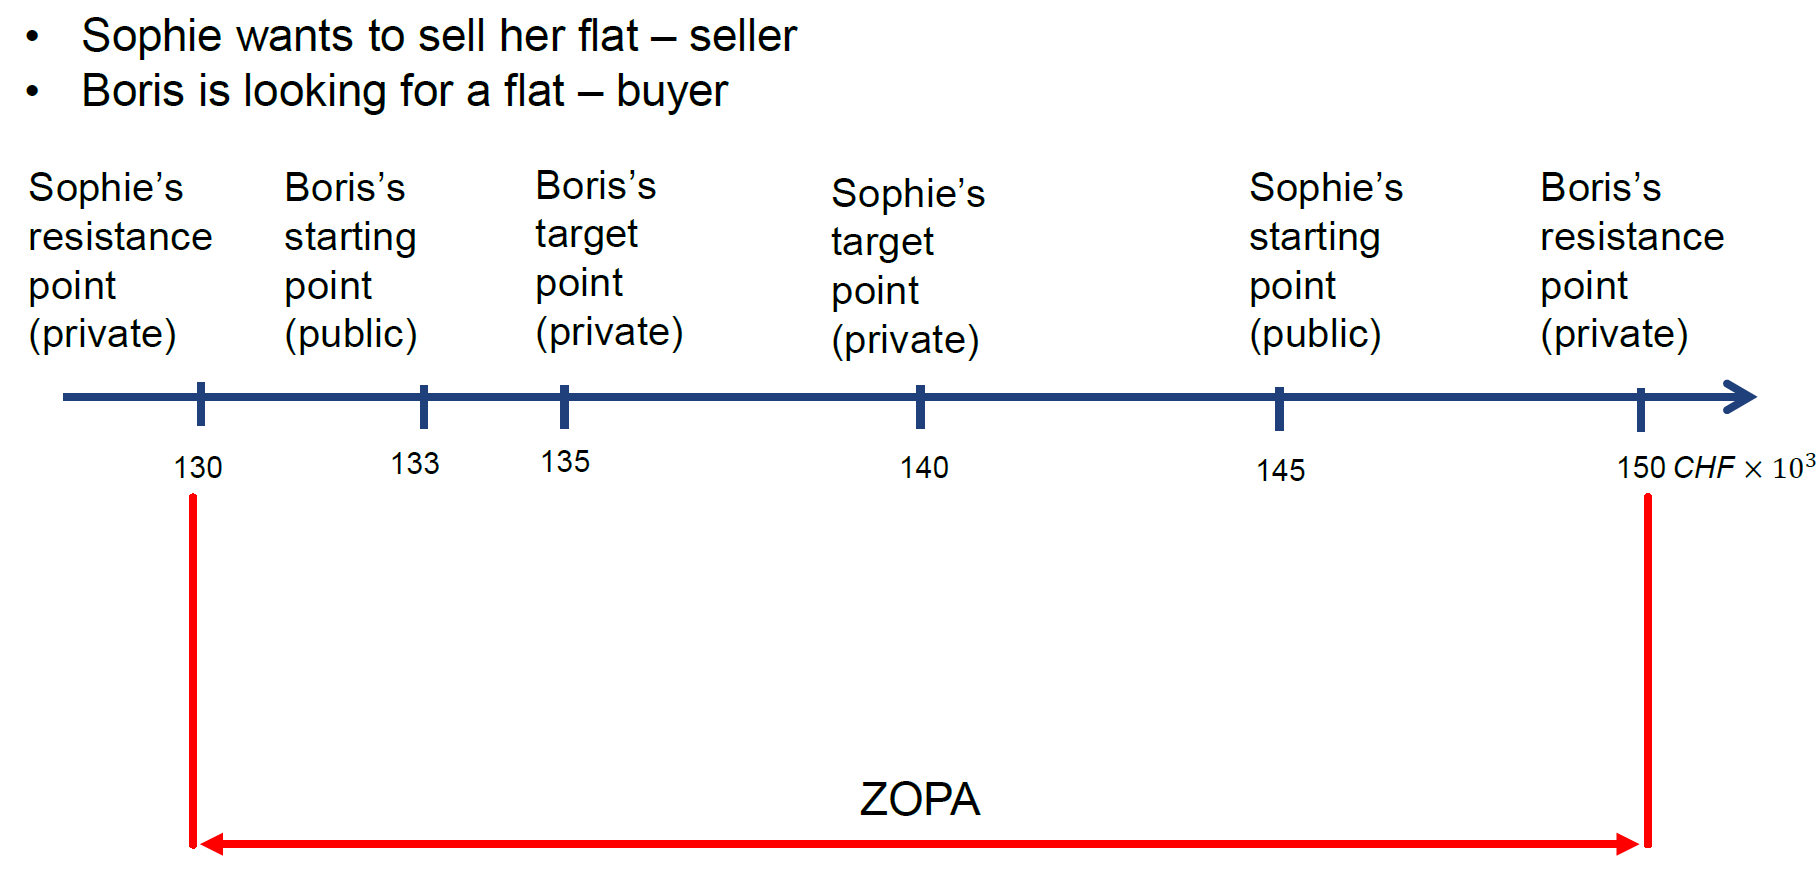
\includegraphics[width=0.5\textwidth]{Pictures/Distributive_negotiation_example_1_1.png}
    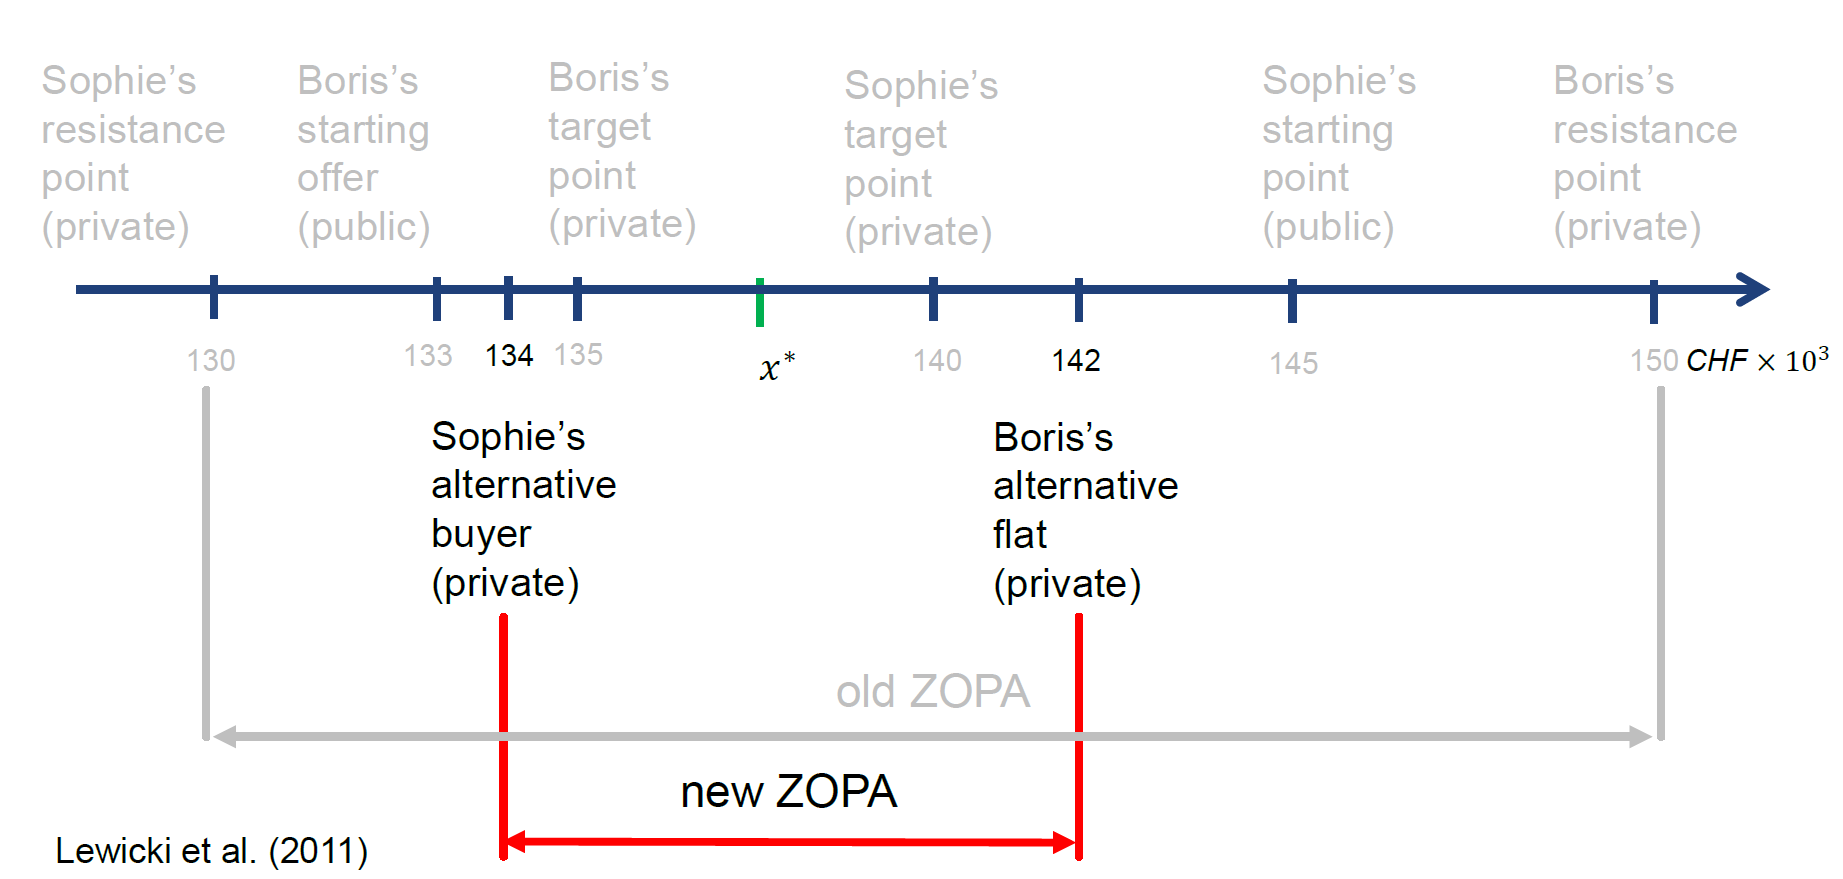
\includegraphics[width=0.5\textwidth]{Pictures/Distributive_negotiation_example_1_2.png}
    \caption{ZOPA without and with alternatives}
\end{figure}

\paragraph{Formal model}

Negotiation:

\begin{itemize}
    \item $b_R$: buyer's resistance point (i.e. the maximum price buyer would agree to pay)
    \item $s_R$: seller's resistance point (i.e. the minimum price seller would settle for)
    \item $x^\ast$: final price
    \item Seller's surplus: $\Delta_S = x^\ast - s_R$
    \item Buyer's surplus: $\Delta_B = b_R - x^\ast$
    \item The total surplus from the deal: $\Delta= \Delta_S + \Delta_B = b_R - s_R$
    \item Note: If $\Delta \geq 0$ there is a ZOPA. If $\Delta < 0$ ther is no ZOPA.
\end{itemize}

\begin{figure}[h]
    \centering
    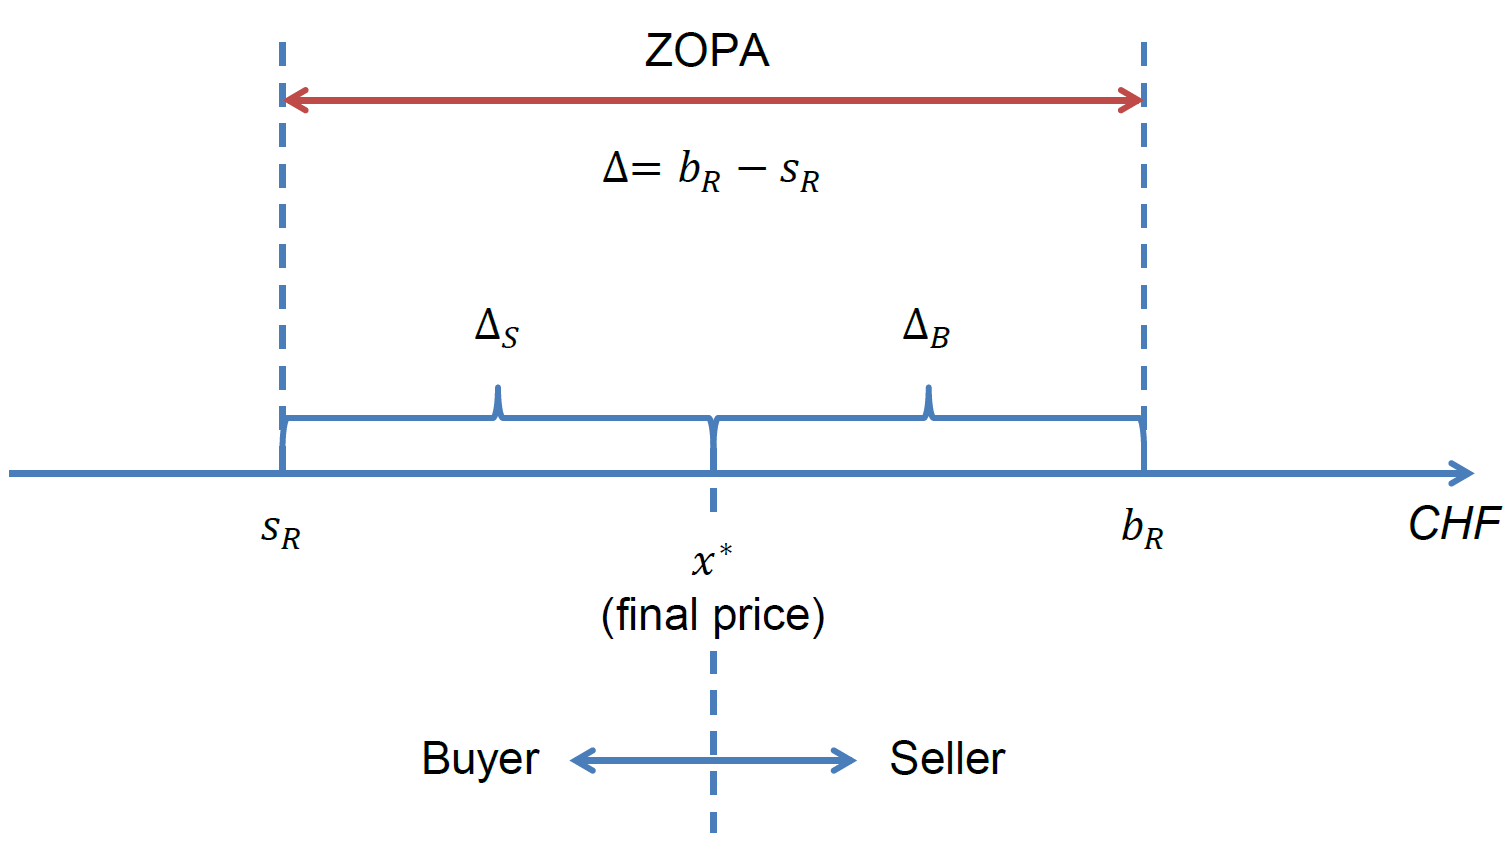
\includegraphics[width=0.5\textwidth]{Pictures/Seller_Buyer_model.png}
    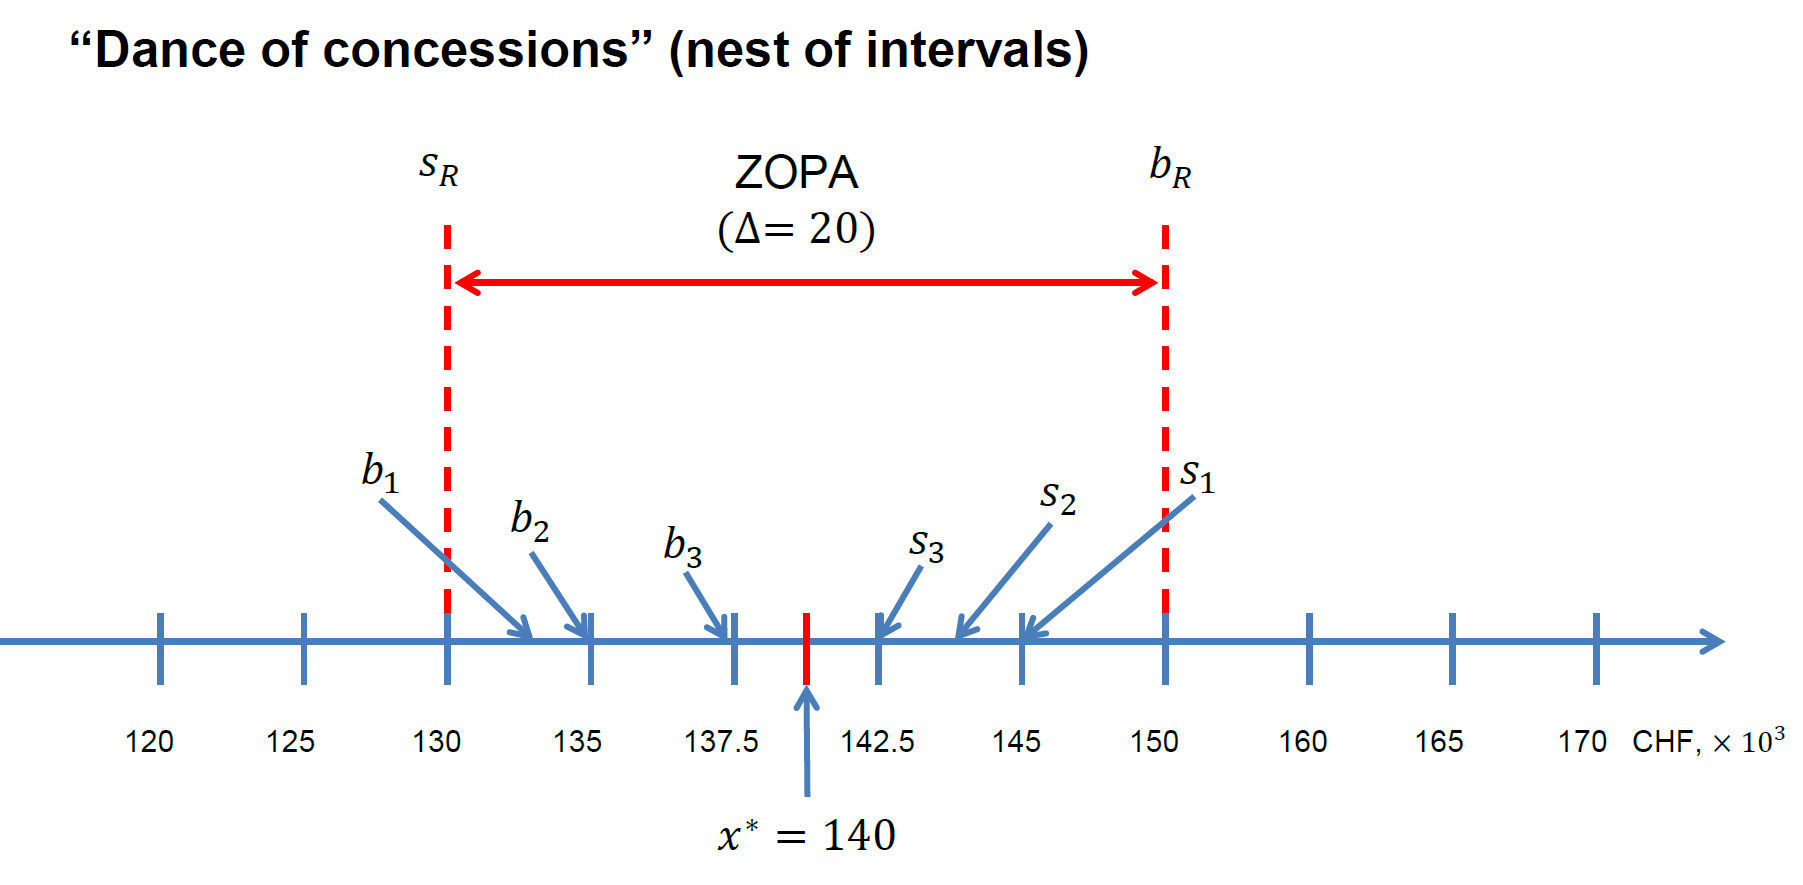
\includegraphics[width=0.5\textwidth]{Pictures/Dance_of_concessions.png}
\end{figure}

\paragraph{Comments}
\begin{itemize}
    \item Achieve the most preferable outcome within the bargaining range
    \item Subjective assessment/perception of the deal
    \item By making high offers and small concessions you can attempt to review the
        resistance points
    \item It is important that people feel as if they got the best possible deal.
\end{itemize}

\subsection{Integrative negotiation}

It is a negotiation that can look for win-win solutions or problem solving
in order to achieve a mutual gain.

\begin{example}[Acquisition of a company]
    \begin{itemize}
        \item A big international corporation (Firm B) wants to make a friendly
            acquisition of one of its suppliers, the small company (Firm S)
        \item Both agree that Firm S would be more valuable as a part of Firm B.
        \item Despite this agreement, they are unable to complete the acquisition.
        \item Firm B offers CHF 13.5 million for Firm S, but firm S insists on CHF
            16.5 million.
        \item Efforts to find a compromise fail: neither side finds 15 CHF acceptable.
    \end{itemize}
\end{example}

\begin{figure}[h]
    \centering
    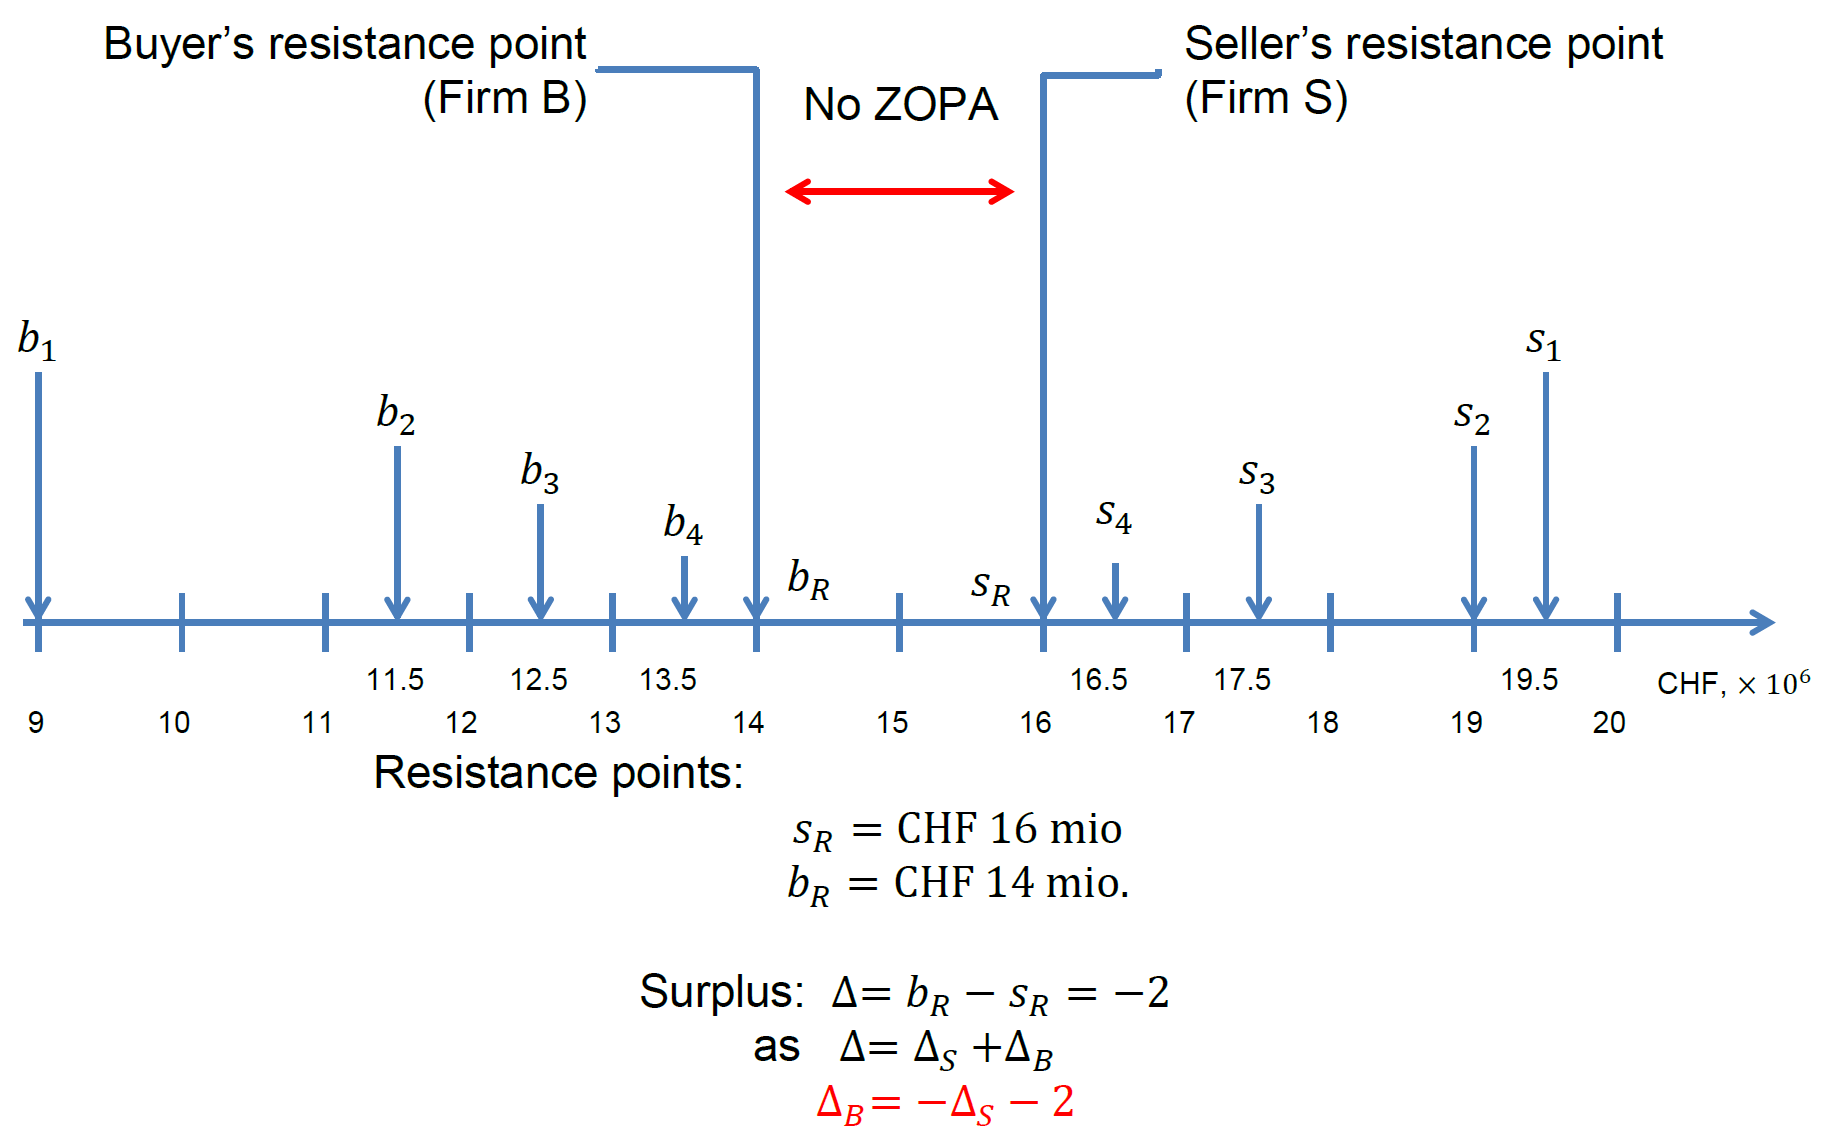
\includegraphics[width=0.5\textwidth]{Pictures/Example_2.png}
\end{figure}

\begin{itemize}
    \item Both firms do some research and realize that the two have different views
        of the value of a new high-tech, high-risk Division D.
    \item Firm B considers Divition D worth only 1 million CHF (of the 14 mio resistance point)
        whilt firm S truly believes in the viability of the new products under development
        and has valued this division at 6 million CHF (of the 16 mio resistance point)
    \item When the parties realize this, they can trade-off on this underlying issue,
        in order to find an agreement: Firm B acquires Firm S for 12 million CHF,
        but the owners of the Firm S retain control of Dividion D.
\end{itemize}

\paragraph{Formal model}

Different valuations of Divition D:
\begin{itemize}
    \item Firm S values it at CHF 6 mio
    \item Firm B values it at CHF 1 mio
\end{itemize}
New resistance points:
\begin{align*}
    s_R &= \text{CHF } 10 \text{ mio } (= 16-6)
    \\
    b_R &= \text{CHF } 13 \text{ mio } (= 14-1)
\end{align*}
Surplus: $\Delta = b_R - s_R = 13-10 = +3$ as $\Delta = \Delta_S + \Delta_B$.
For any price $x^\ast$ the buyer's and seller's surplusses are related to
$\Delta_B = - \Delta_S + 3$. A fair price could be in the middle of 10 and 13 mio.
$x^\ast = 11.5$ mio.

\begin{figure}[h]
    \centering
    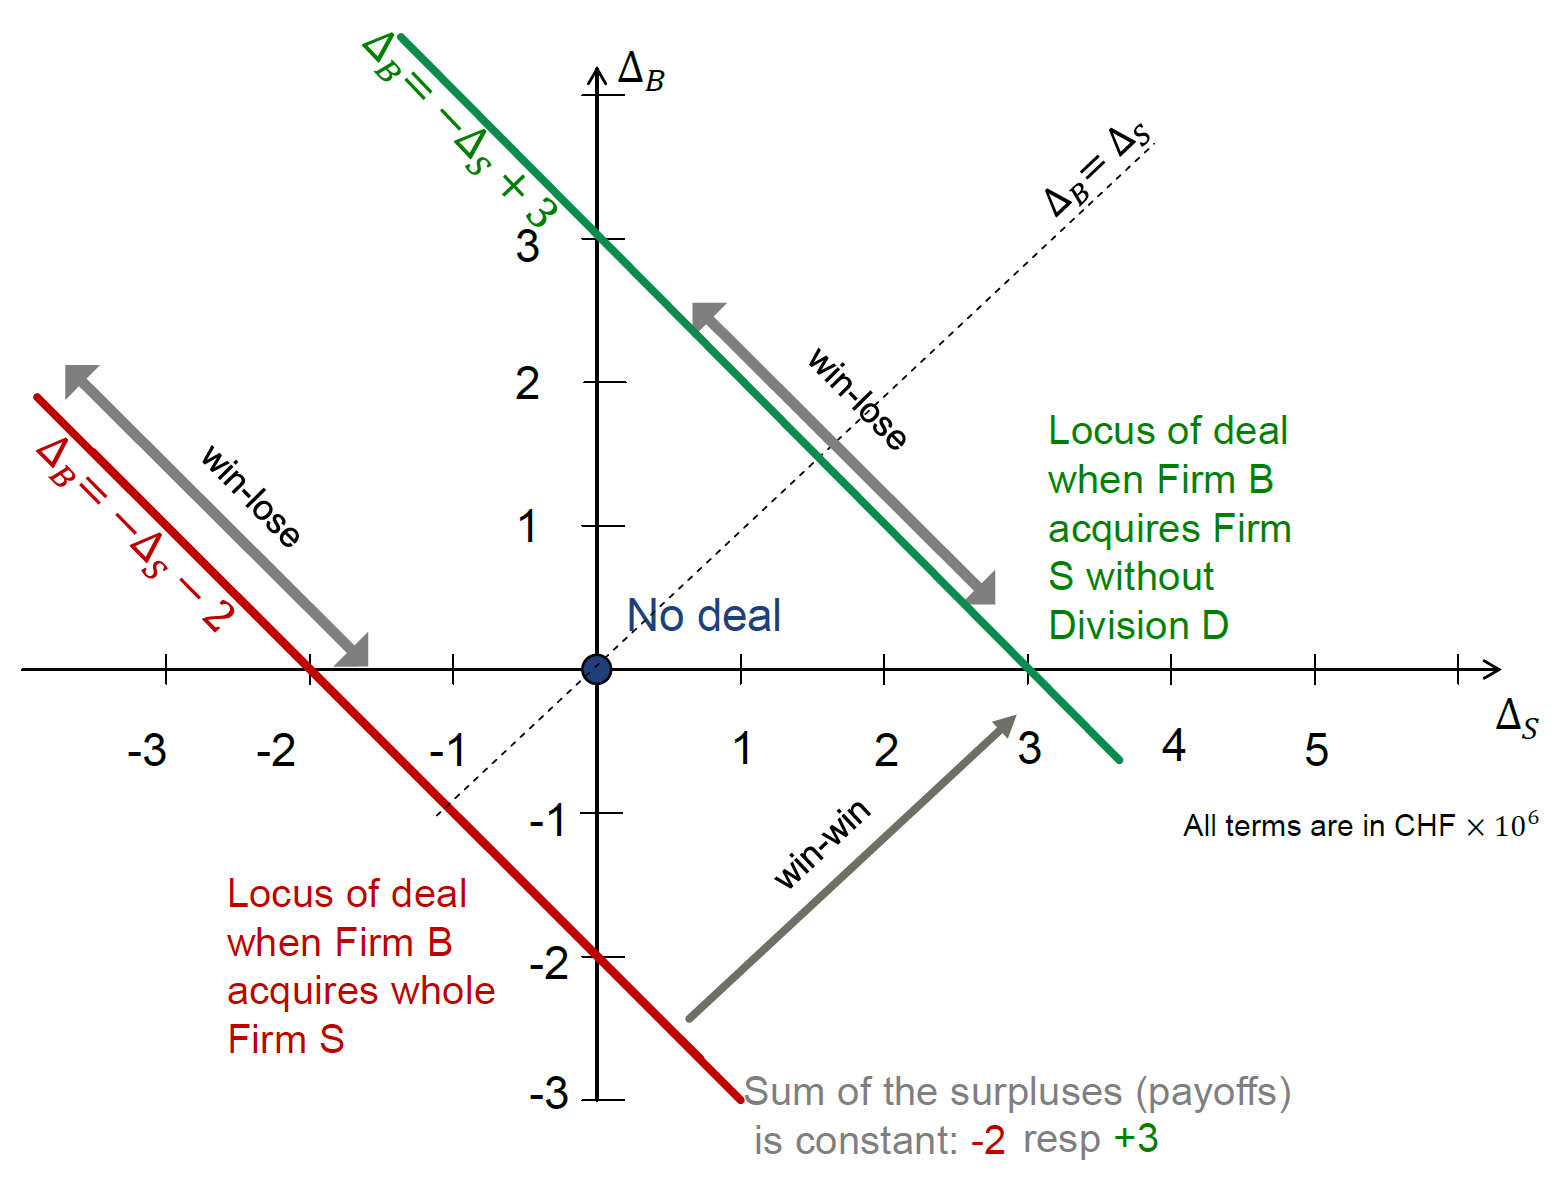
\includegraphics[width=0.5\textwidth]{Pictures/Integrative_negotiation_plot.png}
\end{figure}

\paragraph{Steps in integrative negotiation}

\begin{enumerate}
    \item Sides need to agree on what the problem is
    \item What are the interests behind the positions
    \item Generate alternative solutions
        \begin{itemize}
            \item Redefine the problem (Exapmle 3)
                \begin{itemize}
                    \item Expand pie
                    \item Logroll
                    \item Offer compensation in other area
                    \item minimize costs
                    \item Bridge
                \end{itemize}
            \item Generate solutions for the given problem
        \end{itemize}
    \item Make a list of solutions
    \item Prioritize options and reduce the list
    \item Select a solution
\end{enumerate}

\begin{example}[Generaet alternative solutions]
    \begin{itemize}
        \item The Problem: What will a husband and wife do with 2 weeks of vacation?
        \item Interests:
            \begin{itemize}
                \item She wants: mountains, hiking, and other outdoor activities, rustic cabin
                \item He wants: beach, swimming, and night life, fancy hotel
            \end{itemize}
        \item Generate alternative solution:
            \begin{itemize}
                \item Expand pie: make 4 weeks - 2 weeks mountains; 2 weeks beach
                \item Logrolling: (1) fancy hotel in the mountains or (2) rustic hotel on the beach
                \item Compensation in other area: he pays her a ski equipment, she accepts to go the beach
                \item Minimize cost: he accepts to take a beach house away from the big hotels
                \item Bridge: they choose a place that offres hiking, mountains, swimming, beaches and night life
            \end{itemize}
    \end{itemize}
\end{example}

\paragraph{Comments}
Additional important elements:
\begin{itemize}
    \item Fairnes and other intangibles
        \begin{itemize}
            \item Outcome is equally shared ("divide it down the middle")
            \item Outcome is devided based on equity
            \item Outcome is divided based on needs
        \end{itemize}
    \item Emotional escalation
    \item Difference in risk preferences, expectations, time preferences
    \item "Nothing is agreed until everything is agreed!"
\end{itemize}

\subsection{Best practices}

Lewicki: Ten best practices

\begin{enumerate}
    \item Be prepared
    \item Diagnose the fundamental structure of the negotiation
    \item Work the BATNA (Best alternative to the negotiated agreement)
    \item Be willing to walk away
    \item Master the paradoxes
    \item Remember the intangibles
    \item Actively manage colitions
    \item Savor and protect your reputation
    \item Remember that rationality and fairness are relative
    \item Continue to learn from experience
\end{enumerate}

\pagebreak

\section{Harvard method}

Fundamendal quesion: "What is the best way for people to deal with each other's
differences?"

Problem: Negotiators tend to bargain over positions and lock themselves into
those positions.

Suggested solution: Focus on principled negotiation or negotiation on the
metris instead of positions (e.g. create respective values)

\subsection{Concept}
Negotiation based on five principles:
\begin{enumerate}
    \item People: Separate the people from the problelem
        \begin{itemize}
            \item Negotiation is interaction between people. Be aware of your
                perception, emotions, and communication.
                \begin{itemize}
                    \item Hard on the facts, soft on the people
                    \item Separate the working relationship from the subject of negotiation
                \end{itemize}
        \end{itemize}
    \item Interests: Focus on interest, not positions
        \begin{itemize}
            \item Many negotiations start based on positions. Identify implicit
                and explicit interests of negotiations behind the positions.
                \begin{itemize}
                    \item Position: manifestation of an interest in a concrete manner.
                    \item Interest: unterlying motivation, concern, and importance
                \end{itemize}
            \item Examples: Window opening, Two sisters want an orange but there
                is only one left (orange peel), 1978 Israeli-Egyptian peace talks after
                6 Day War 1967, Camp David.
        \end{itemize}
    \item Options: Invent options for mutual gain
        \begin{itemize}
            \item Invent and judge options for potential solutions with the aim
                to create mutual gain.
        \end{itemize}
    \item Criteria: Insist on using objective criteria
        \begin{itemize}
            \item Develop, agree upon and apply objective criteria upon which an
                agreement can be derived.
        \end{itemize}
    \item Alternatives: Know your best alternative to a negotiated agreement (BATNA)
        \begin{itemize}
            \item Be aware under which condition an agreement is not in your favor.
        \end{itemize}
\end{enumerate}

\subsection{Criticism}

\begin{itemize}
    \item Not much beyond common sense (professional negotiators are alerady doing this)
    \item It is not scholarly or analytical and relies on anecdotal evidence
    \item It is too simplified for complex situations
    \item "The authors seem to deny the existence of a significant part of the
        negotiation process, and to oversimplify of explain away many of the most
        troublesome problems inherent in the art of practice of negotiation"
\end{itemize}

\pagebreak

\section{Game Theory}

\paragraph{Possiblities}
\begin{itemize}
    \item Individual decision-making (Games with $N=1$)
    \item Group of $N$ individuals (Games with $N>1$)
        \begin{itemize}
            \item Non cooperative games
                \begin{itemize}
                    \item Static games
                        \begin{itemize}
                            \item Constant sum game (zero-sum):
                                Pure Strategy and Mixed Strategy
                                % \begin{itemize}
                                %     \item Pure Strategy
                                %     \item Mixed Strategy
                                % \end{itemize}
                            \item Non constant sum game
                        \end{itemize}
                    \item Dynamic games:
                        Sequential move games and repeated simultaneous move games
                        % \begin{itemize}
                        %     \item Sequential move games
                        %     \item Repeated simultaneous move games
                        % \end{itemize}
                \end{itemize}
            \item Cooperative games
        \end{itemize}
\end{itemize}

\subsection{Introduction}

Two generals opposing each other in a battle. Each has the possibility to
attack or withdraw.

\begin{figure}[h]
    \centering
    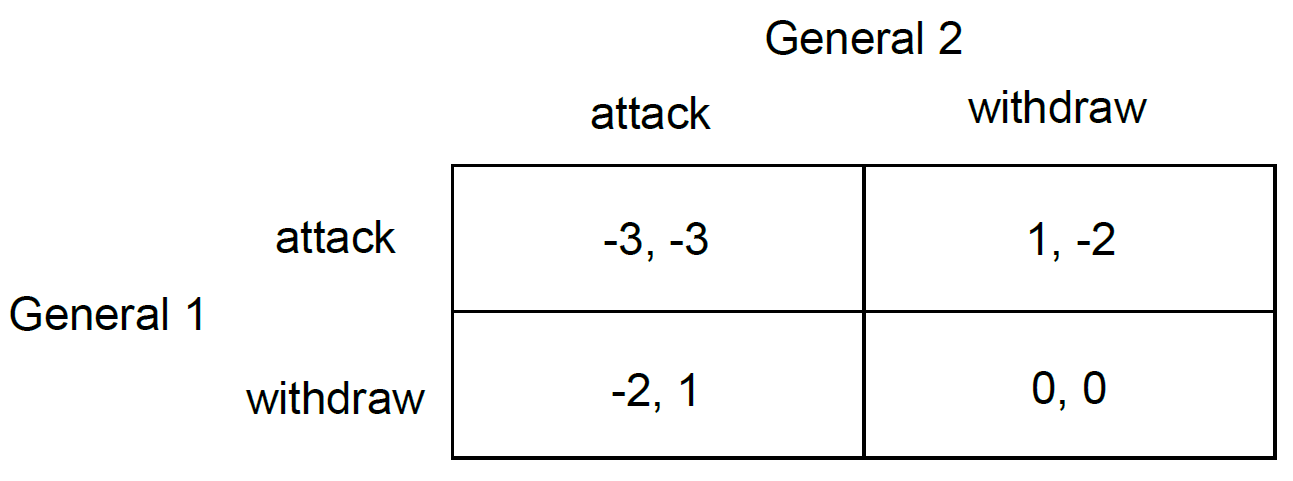
\includegraphics[width=0.4\textwidth]{Pictures/two_generals_GT.png}
\end{figure}

According to Adam Smith: "In competition, individual ambition serve the common
good."

Contrary to this: Nash's key sentence: "The best result comes from everyone in
the group doing what is best for himself \underline{and} the group."

\subsubsection{History}
John von Neumann (1903-1957)
\begin{itemize}
    \item Born in Budapest
    \item Diploma in chemical engineering from ETH (1926)
    \item PhD in mathematics from University of Budapest
    \item Founded the field of game theory as a mathematical discipline
\end{itemize}

Oskar Morgenstern (1902-1977)
\begin{itemize}
    \item Born in Görlitz (Germany)
    \item Student and PhD in political sciences at University of Vienna
    \item Together with Neumann, he founded the mathematical field of game
        theory and its application to economics.
\end{itemize}

John Nash (1928-2015)
\begin{itemize}
    \item Born in Bluefield (USA)
    \item Master in Mathematics from Carnegie Mellon University
    \item PhD in Mathematics from Princeton University
    \item Defined and studied what would later be called the "Nash equilibrium"
        and the "Nash bargaining solution"
    \item Nobel prize 1994; Abel prize 2015
\end{itemize}


\subsubsection{What is Game Theory?}

Roger Myerson:
"Game theory can be defined as the study of mathematical
models of conflict and cooperation between intelligent
rational decision-makers. Game theory provides general
mathematical techniques for analyzing situations in which
two or more individuals make decision that will influence one
another’s welfare. […] Game theory offers insights of
fundamental importance for scholars in all branches of the
social sciences, as well as for practical decision-makers."

\subsection{Individual decision-making (Games with $N=1$)}

\begin{example}[Linear programming: production problem]
\end{example}

\begin{figure}[h]
    \centering
    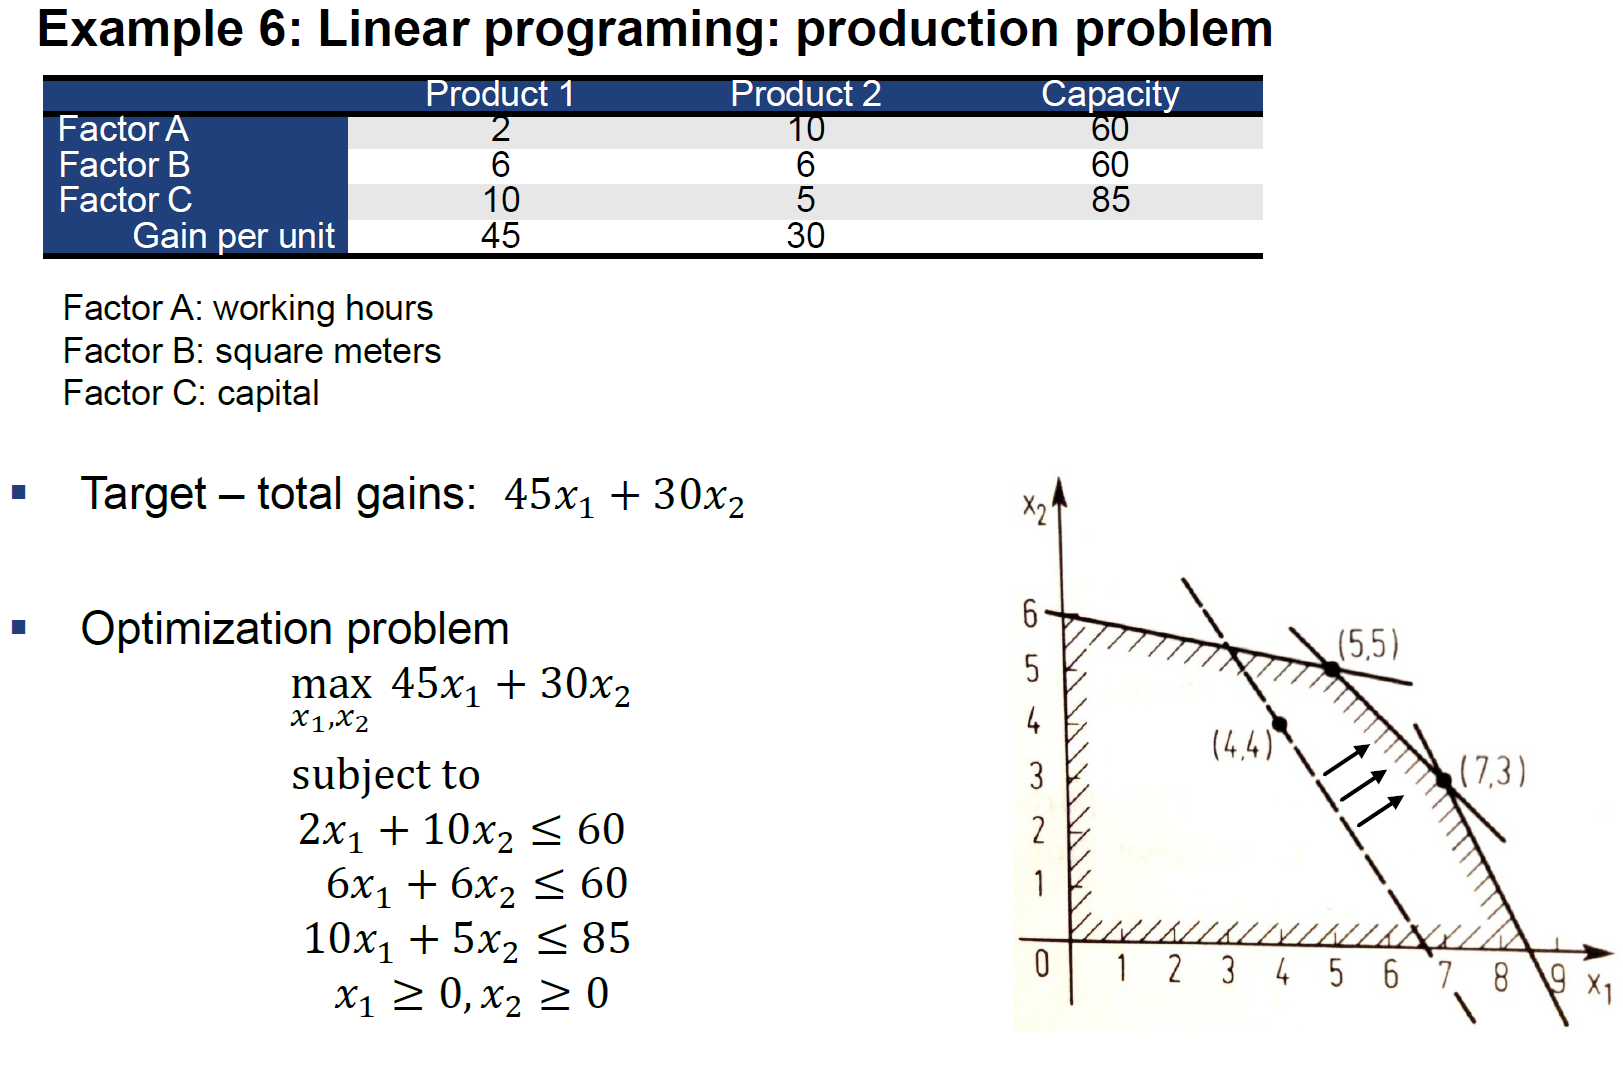
\includegraphics[width=0.45\textwidth]{Pictures/Linear_programming_1.png}
    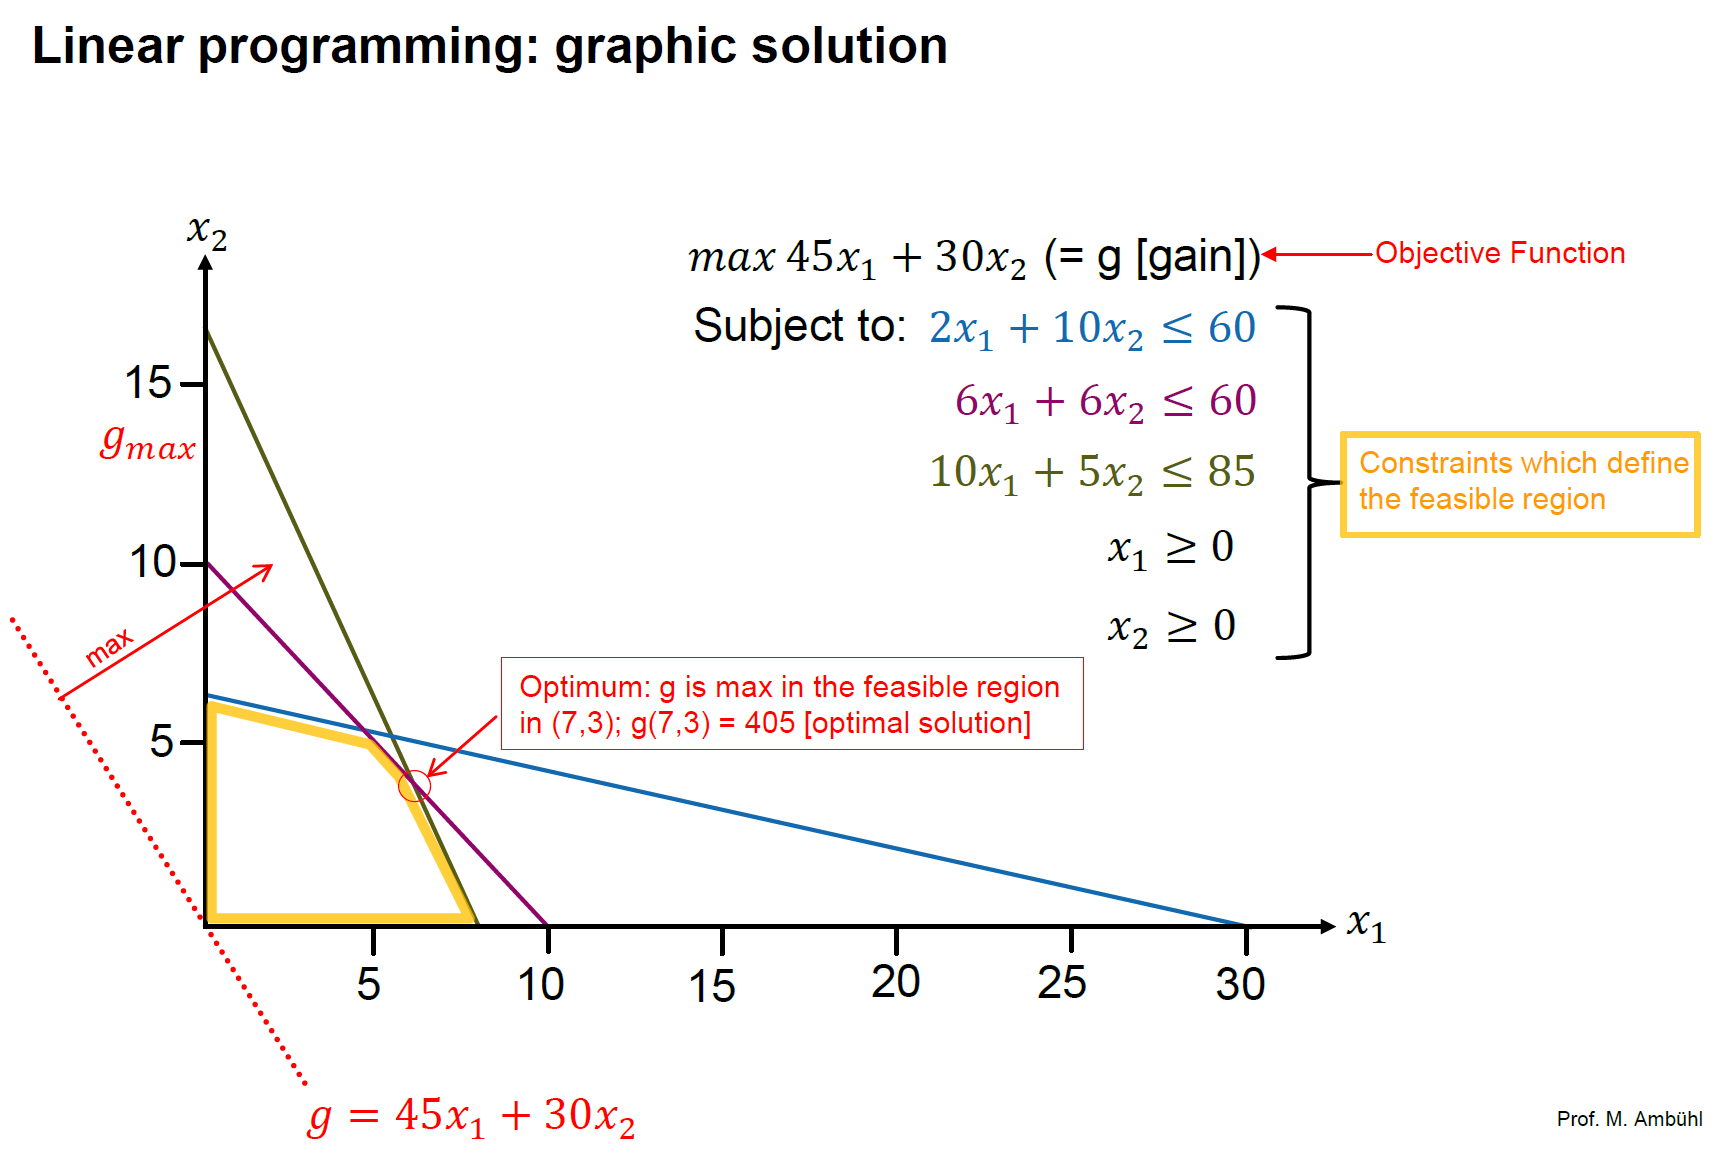
\includegraphics[width=0.45\textwidth]{Pictures/Linear_programming_2.png}
\end{figure}

\begin{example}[Secretary problem]
    There exists different versions of the problem. Here is an easy version:
    \begin{itemize}
        \item There is one secretarial position available
        \item The number of $n$ of applicants is known
        \item The applicants are interviewd sequentially in random order
        \item Each time you see an applicant you have to decide if you take him/her
            or not. The rejection of an applicant cannot be revoked later on. If
            you decide on taking one applicant you can not see any other applicant
            thereafter.
        \item You compare each candidate with the ones you have already seen
        \item $\Rightarrow$ How should you proceed in order to maximize the probablity
            of selecting the \underline{best} candidate?
        \item You should let $\frac{n}{e}$ applicants go by and then select the first
            one whose value exceeds those of all the earlier rejected ones. The probablity
            of getting the best one with this strategy is $\frac{1}{e} \approx 37\%$
        \item Proof:
            \begin{itemize}
                \item $n$ applicants ($n$ is known) are to be presented in a randomized
                    Sequential order
                \item When an applicant is in front of you, you must either chose him,
                    and the game is over, or you reject him, and you can't go back.
                \item The probablity to choose the best is at each stage $\frac{1}{n}$.
                \item Suppose you reject the first candidate, then there is a $\frac{1}{n}$
                    chance that this one was the best and you failed to select the best
                \item The second now presents himself and you compare him to the first. If
                    he is not as good as the first you will obviously not select him; but
                    even if the second is better than the first, you might still want to pass
                    up on that person because you think the best is among the remaining ones
                \item The best of the rejected ones serves you as the standard for judging
                    the ones to come. So the best of the first $x$ ($x$: rejected ones) will
                    represent a standard against which to judge the remainder.
                \item How many should you let go before making your choice? What chance do you
                    have to pick the best?
                    \begin{itemize}
                        \item \underline{Strategy S}: Idea: Divide the universal sequence of
                            all candidates into two groups; the first group (called the rejected
                            ones or the “standard-setting group”) consisting of a proportion $t$
                            of candidates, is used only toidentify the best in that group; we then
                            sequentially observe the candidates in the second group (called the
                            selection group)and choose the first who beats the best in the
                            standard-setting group. $P(t)$:Probability of finding the best
                            candidate when the standard-setting group comprises a proportion
                            of t candidates. This stragegy will result in the choice of the best, if
                            \begin{itemize}
                                \item the second best falls in the first group (proportion $t$,
                                    $0 \leq t \leq 1$) and the first best in the second
                                    (proportion $(1-t)$). This has the probability $p = t (1-t)$.
                                \item the third best falls in the first group (probability $p=t$)
                                    and the first best in the second group ($p = (1-t)$) and the second
                                    best also in the second group ($p=(1-t)$), and the first comes
                                    before the second ($p=\frac{1}{2}$). This has probability of
                                    $p = t \frac{(1-t)^2}{2}$.
                                \item the fourth best falls in the first segment and the first,
                                    second, and third best in the second segment and the first comes
                                    before the second or the third: $p = \frac{t (1-t)^3}{3}$
                                \item and so on\dots
                                \item Hence: $P(t) = t (1-t) + \frac{t(1-t)^2}{2} + \frac{t (1-t)^3}{3} + \dots$ assuming $n \rightarrow \infty$:
                                    $P(t) = t \eckigeklammer{(1-t) + \frac{(1-t)^2}{2} + \frac{(1-t)^3}{3} + \dots}
                                            = - t \ln(t)$
                                \item To find the optimal proportion for the standard-setting
                                    group, we differentiate $P(t)$ and set $P'(t)$ to $0$. This
                                    yields: $t = \frac{1}{e}$, so $P\klammer{\frac{1}{e}} = \frac{1}{e}$
                            \end{itemize}
                    \end{itemize}
            \end{itemize}
        \item Concrete Case, $n$ small ($n=4$):
            \begin{itemize}
                \item You want to select the best candidate, only the best
                \item Random order, each order being equally likely
                \item You can rank all applicants from worst to best; the
                    decision to accept or reject is based only on the relative
                    rank
                \item Let $n=4$
                \item Best candidate: rank 4; least best candidate: rank 1
                \item Ranks are ordinal numbers
                \item $n!$ permutationspossible, i.e. $4 \cdot 3 \cdot 2 \cdot 1=24$
                \item Strategy: Let $t$ ($0 \leq t < 4$) applicants pass by, then
                    select the first one that is better than the rejected one(s)
                \item $\frac{4}{e} \approx 1.471$, rounded: $t=1$.
            \end{itemize}
    \end{itemize}
\end{example}

\begin{figure}[h]
    \centering
    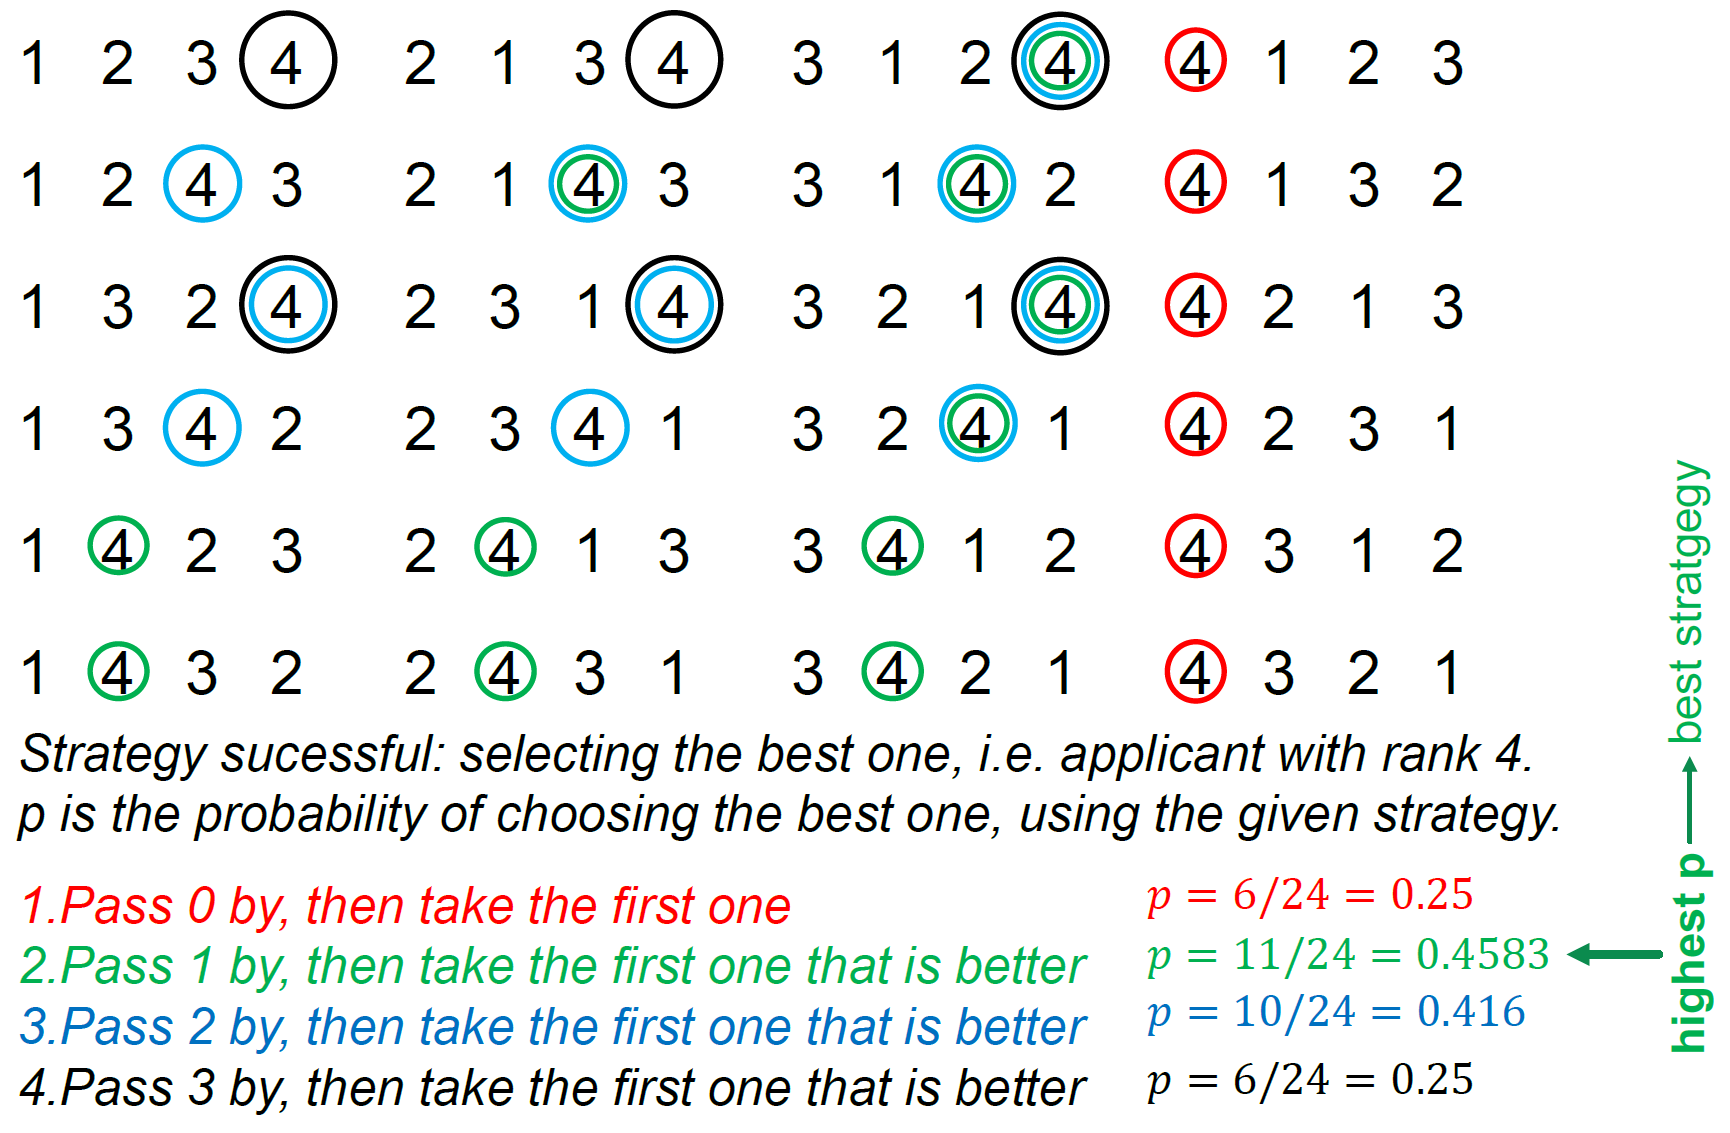
\includegraphics[width=0.35\textwidth]{Pictures/secretary_problem_n_4.png}
\end{figure}

\begin{minipage}{0.45\textwidth}
    \paragraph{Example $8$: Casino (Game against nature)}
    \begin{itemize}
        \item You have four actions: A, B, C, and D
        \item Choices of nature: W, X, Y, and Z
    \end{itemize}
\end{minipage}
\begin{minipage}{0.45\textwidth}
    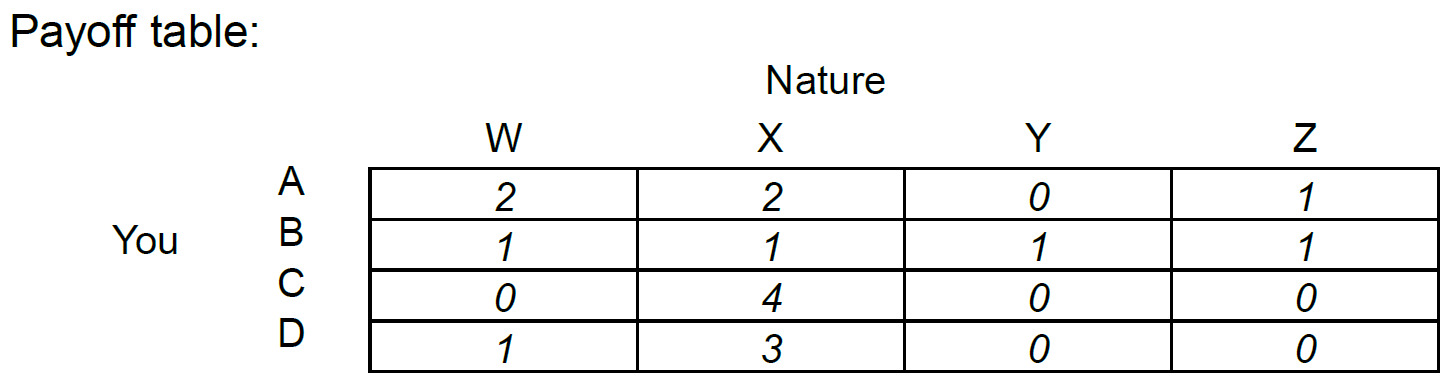
\includegraphics[width=0.9\textwidth]{Pictures/Payoff_table.png}
\end{minipage}

\begin{figure}[H]
    \centering
    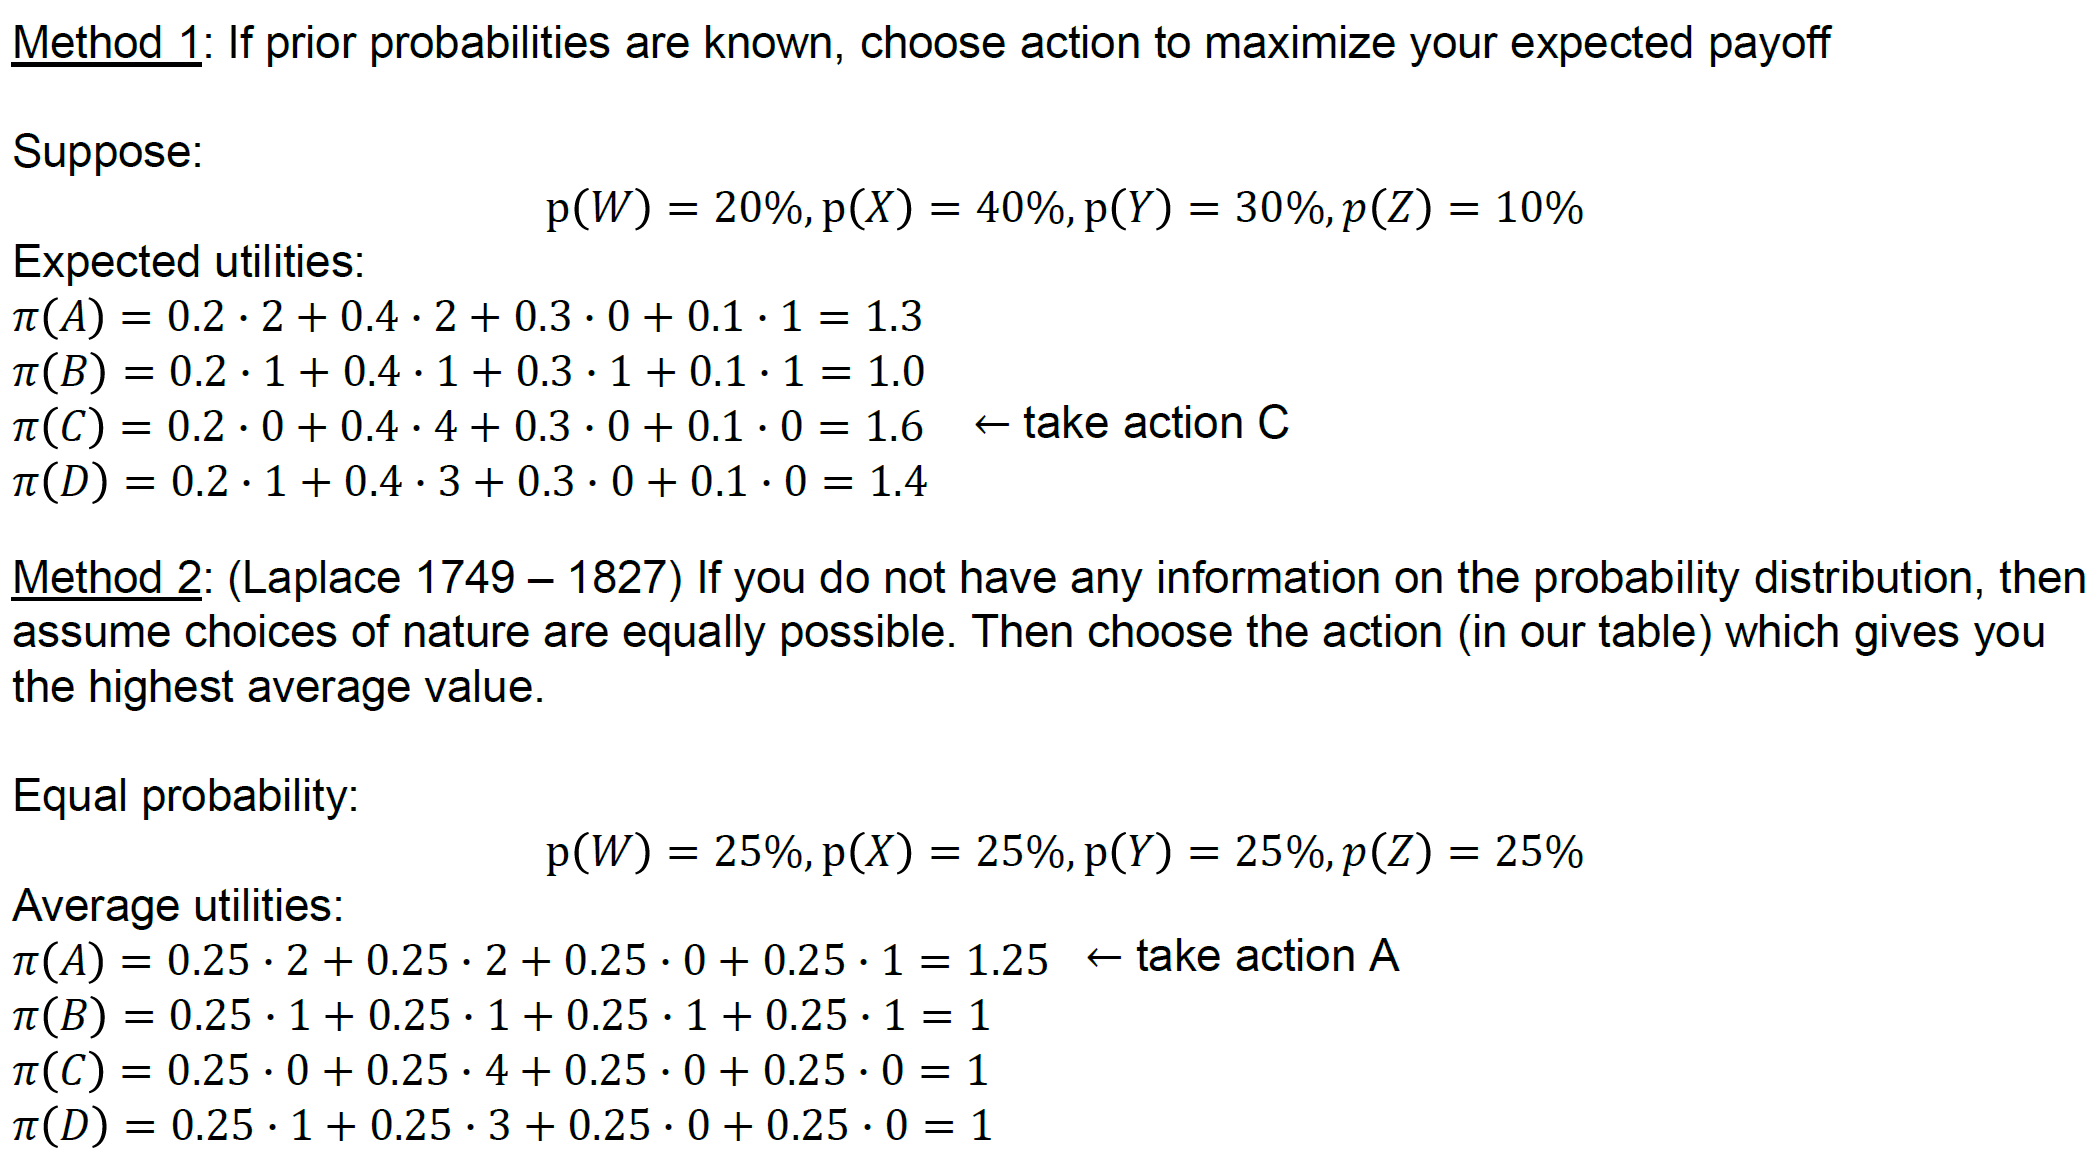
\includegraphics[width=0.6\textwidth]{Pictures/method_1_and_2.png}
    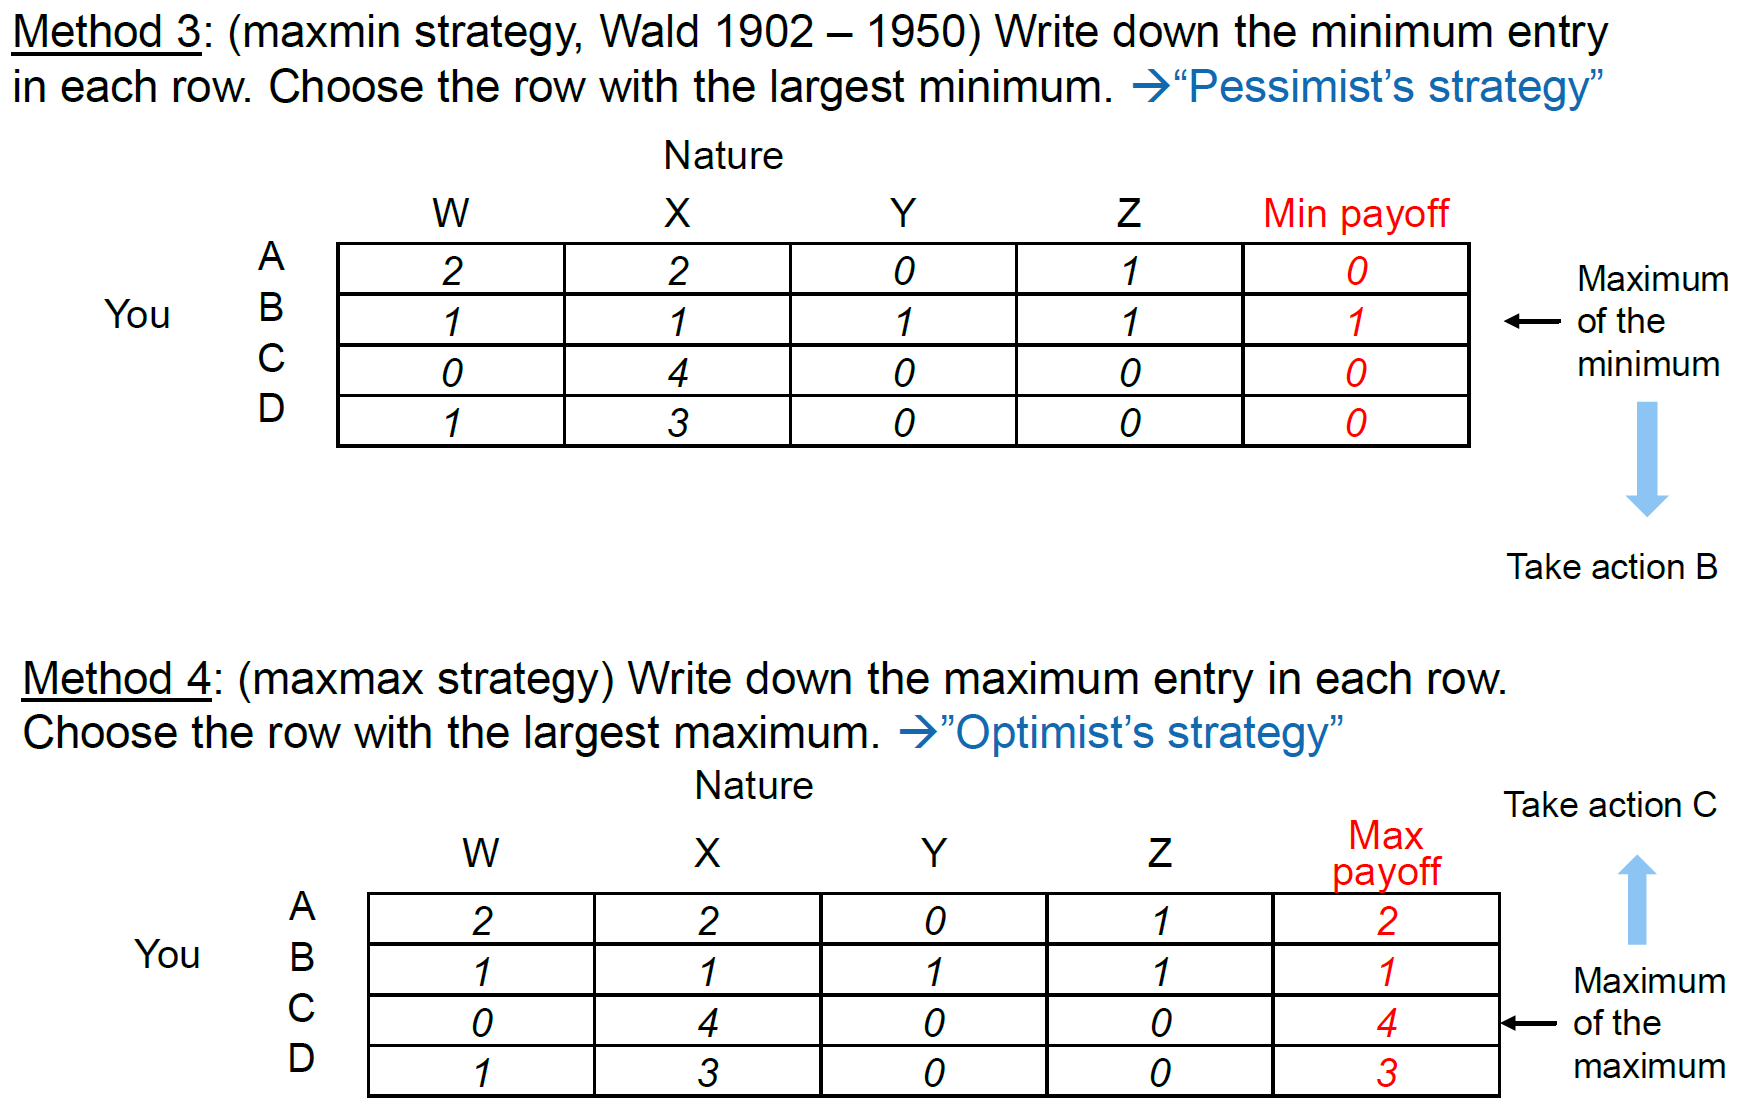
\includegraphics[width=0.6\textwidth]{Pictures/Method_3_and_4.png}
    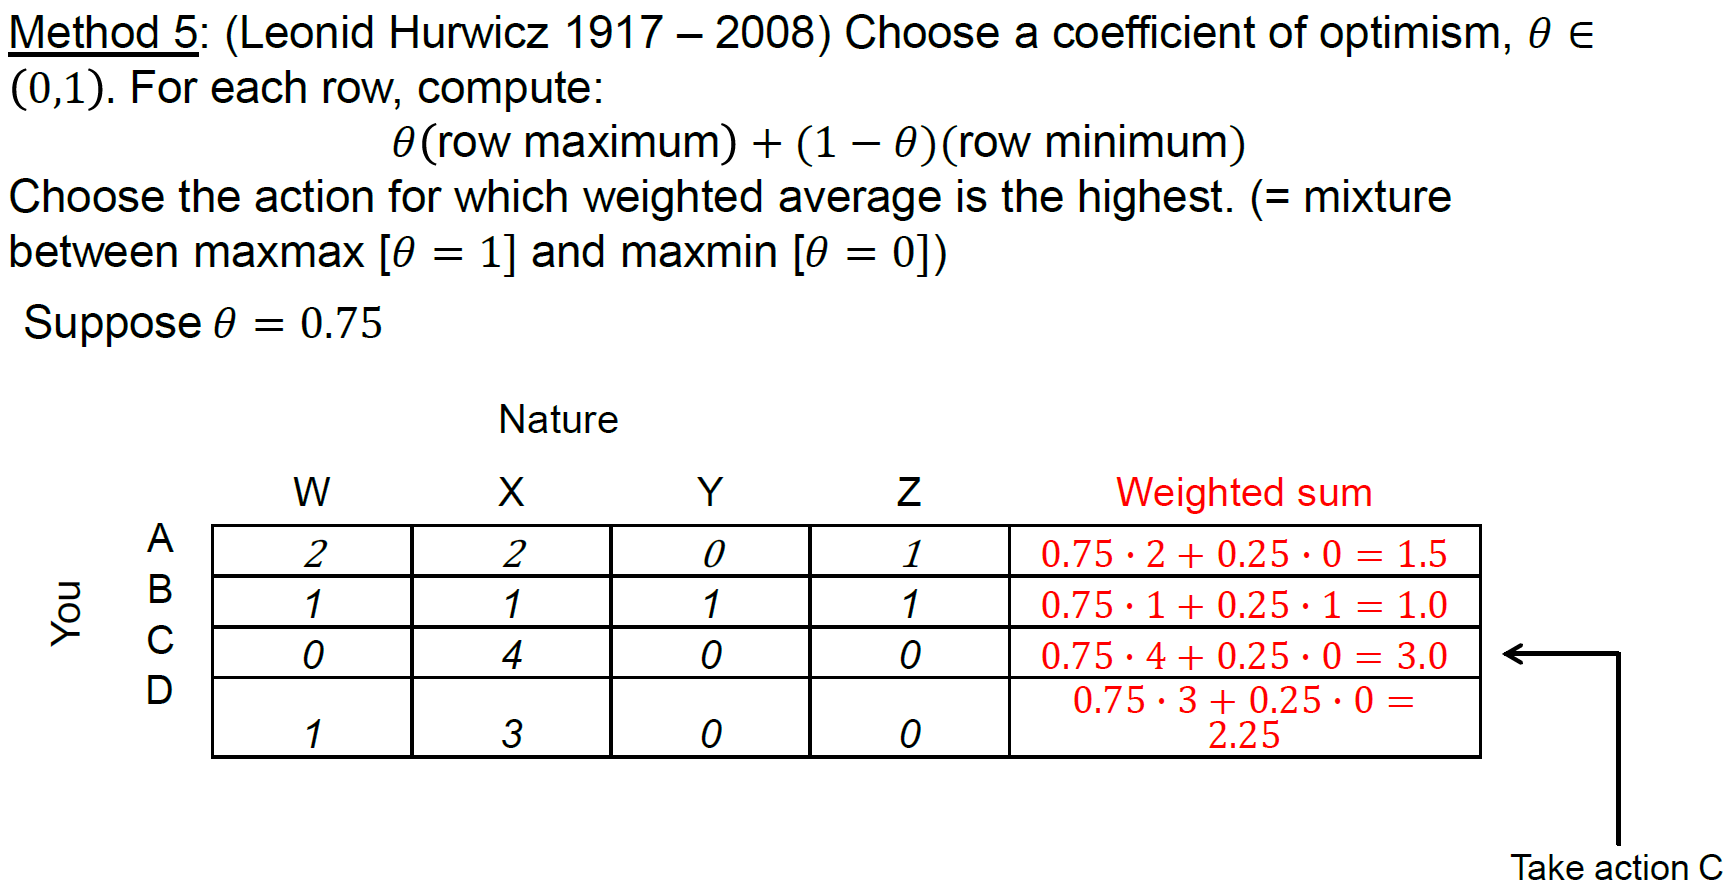
\includegraphics[width=0.6\textwidth]{Pictures/method_5.png}
    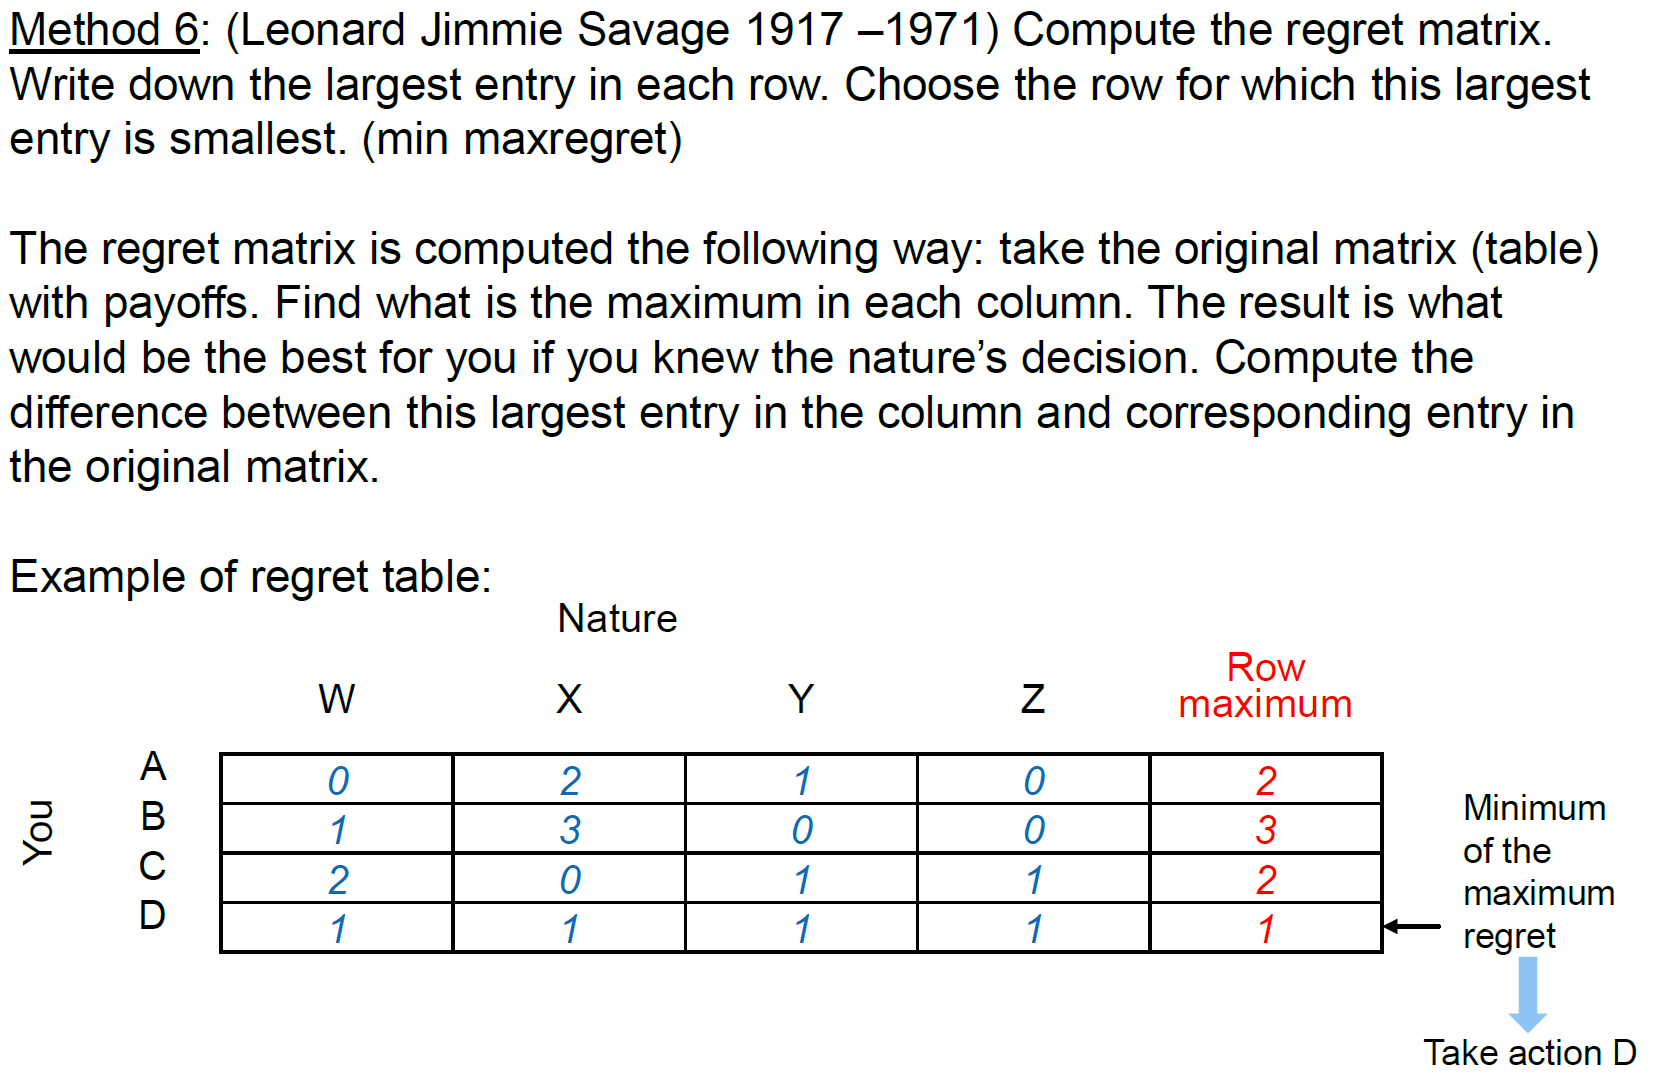
\includegraphics[width=0.6\textwidth]{Pictures/method_6.png}
\end{figure}

\begin{figure}[H]
    \centering
    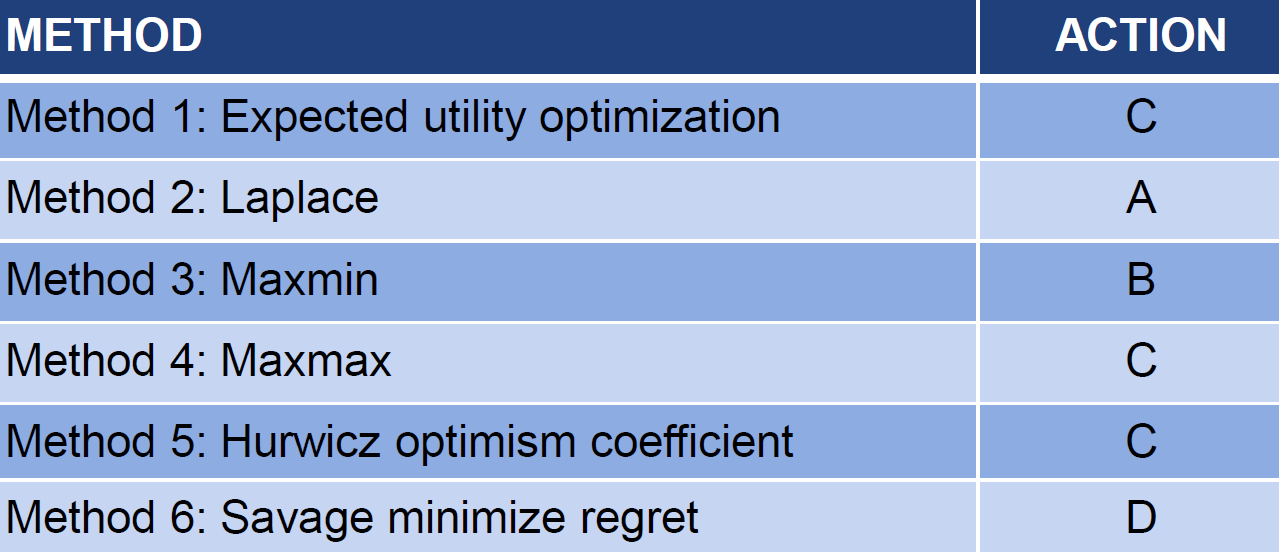
\includegraphics[width=0.5\textwidth]{Pictures/results_method.png}
\end{figure}

\subsection{Group of $N$ individuals (Game with $N>1$)}

\subsubsection{Non cooperative Games}

\paragraph{Static Games}

\begin{itemize}
    \item The Players:
        Who is involved?
    \item The rules:
        \begin{itemize}
            \item Who moves when?
            \item What do they know when they move?
            \item What can they do?
        \end{itemize}
    \item The outcomes: For each possible set of actions by the players what
        is the outcome of the game?
    \item The payoffs: What are the players' preferences (i.e. utilities) over
        the possible outcomes?
    \item Pure strategies - there is no randomization when players take an action.
\end{itemize}

\subparagraph{Constant sum Game}

Pure Strategy:

Example 9: Boris and Sophie divide the surplus

\begin{enumerate}[a)]
    \item Situation in words
        \begin{itemize}
            \item Imagine Sophie and Boris decide to finalize a price in the following manner:
            \item They sit in different rooms, don’t communicate with each other and announce their decision simultaneously: A or B
            \item If both announce A they trade without concessions (i.e. each gets zero additional surplus)
            \item If Boris announces B and Sophie –A : The price will shift towards Sophie by CHF 5
            \item If Boris announces A and Sophie –B: The price will shift towards Boris by CHF 4
            \item If both announce B: Sophie will make a concession towards Boris by CHF 1
        \end{itemize}
    \item Game
        \begin{enumerate}[(i)]
            \item Players: 2 (Boris, Sophie)
            \item Actions: 2 (A,B)
            \item Preferences: Boris: $(A,B) \succ (B,B) \succ (A,A) \succ (B,A)$,
                Sophie: $(A,B) \prec (B,B) \prec (A,A) \prec (B,A)$
            \item Payoffs are presented in the normal form below
            
                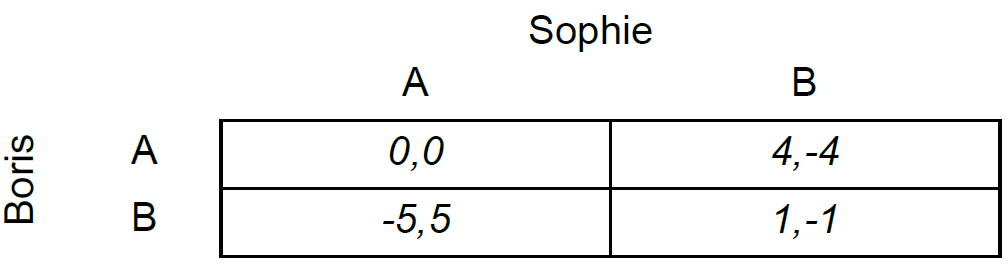
\includegraphics[width=0.4\textwidth]{Pictures/boris_sophie_game.png}
            \item Zero sum Game.
        \end{enumerate}
\end{enumerate}

\begin{figure}[H]
    \centering
    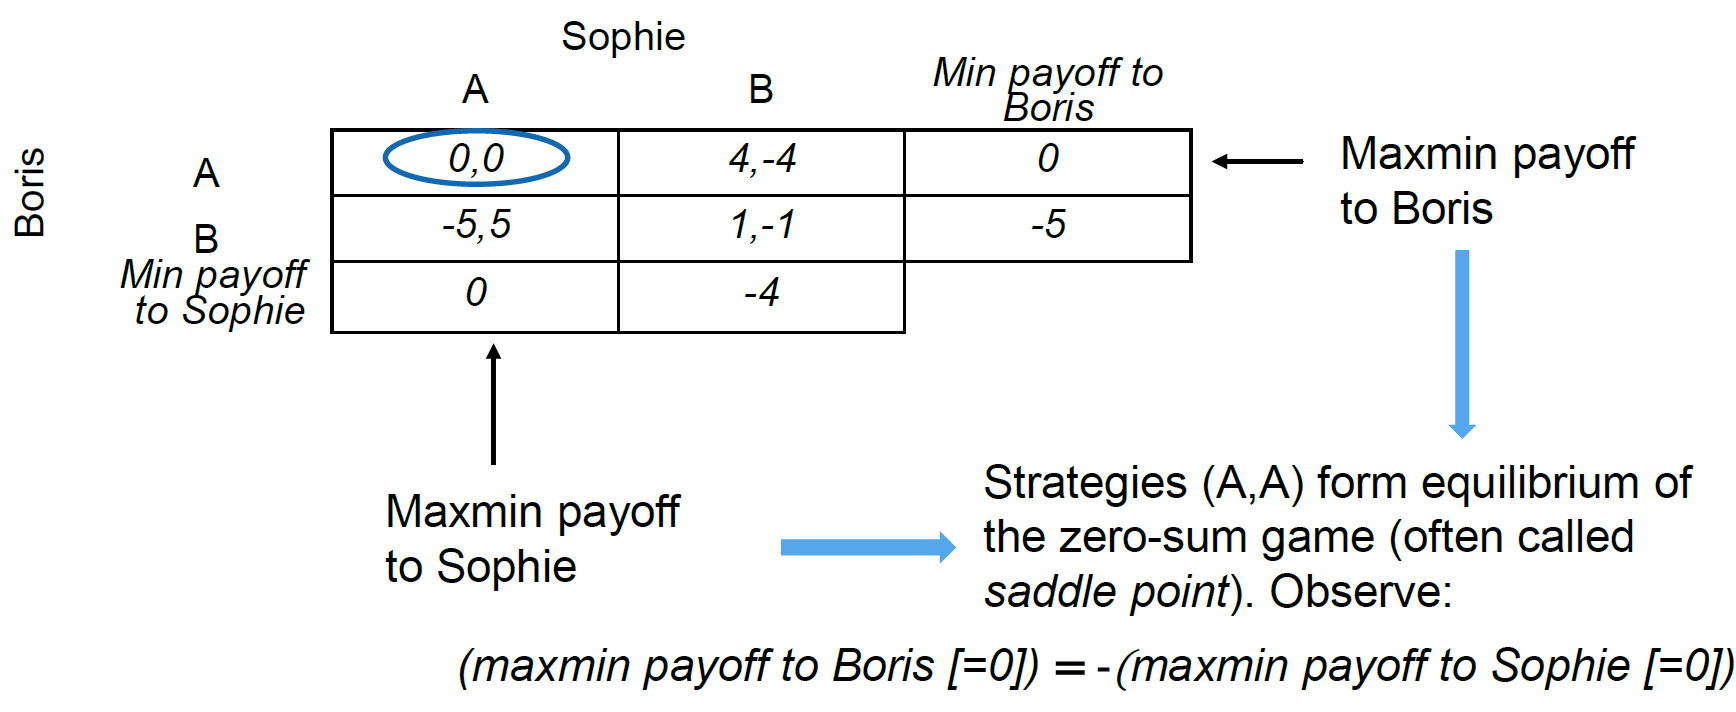
\includegraphics[width=0.5\textwidth]{Pictures/maxim_analysis_saddle_point.png}
\end{figure}

\begin{figure}[H]
    \centering
    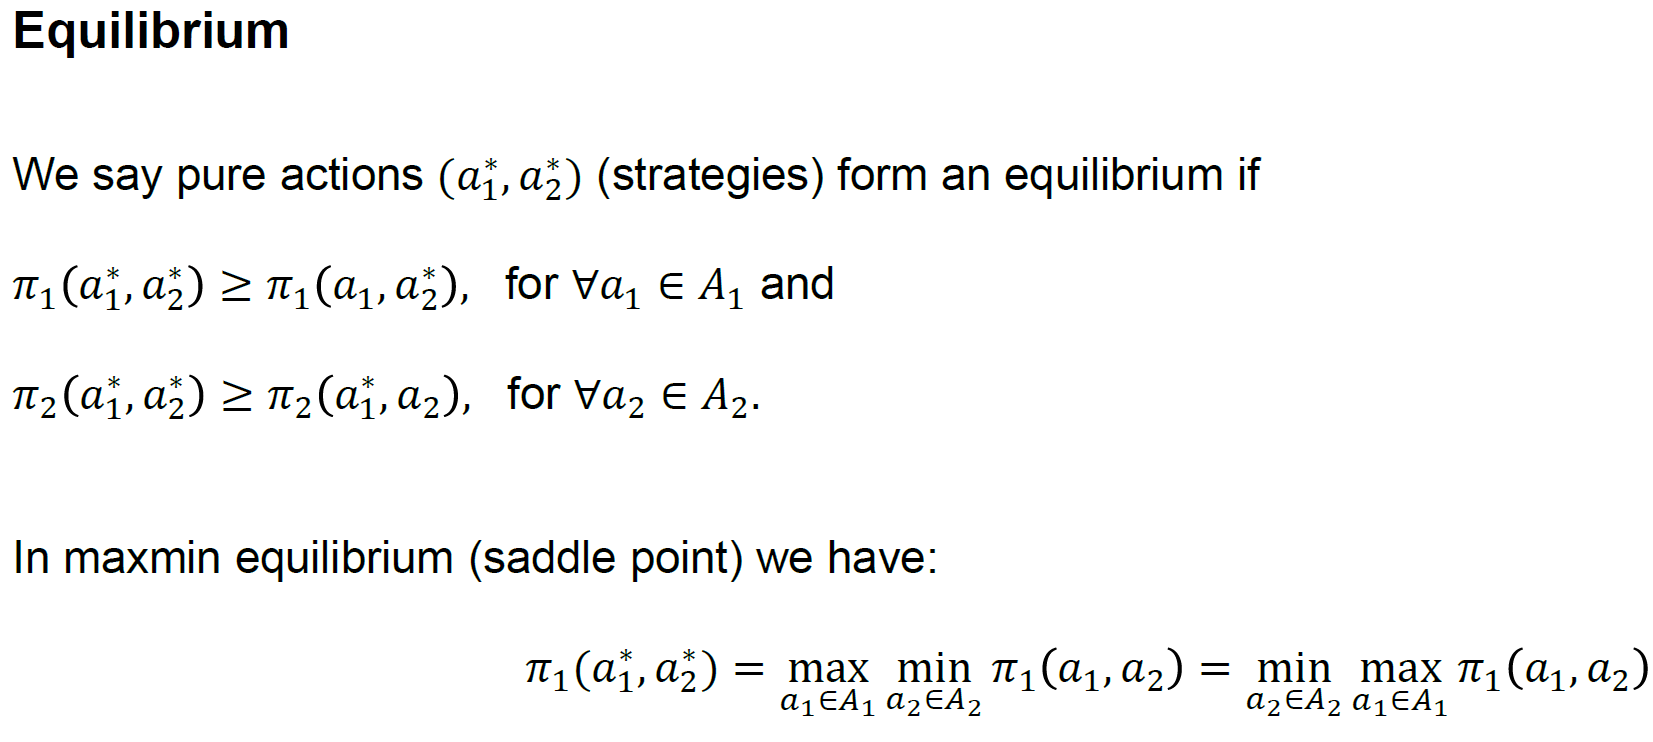
\includegraphics[width=0.5\textwidth]{Pictures/equilibrium.png}
\end{figure}

\begin{theorem}[Maxmin (John von Neumann)]    
\end{theorem}

\begin{figure}[H]
    \centering
    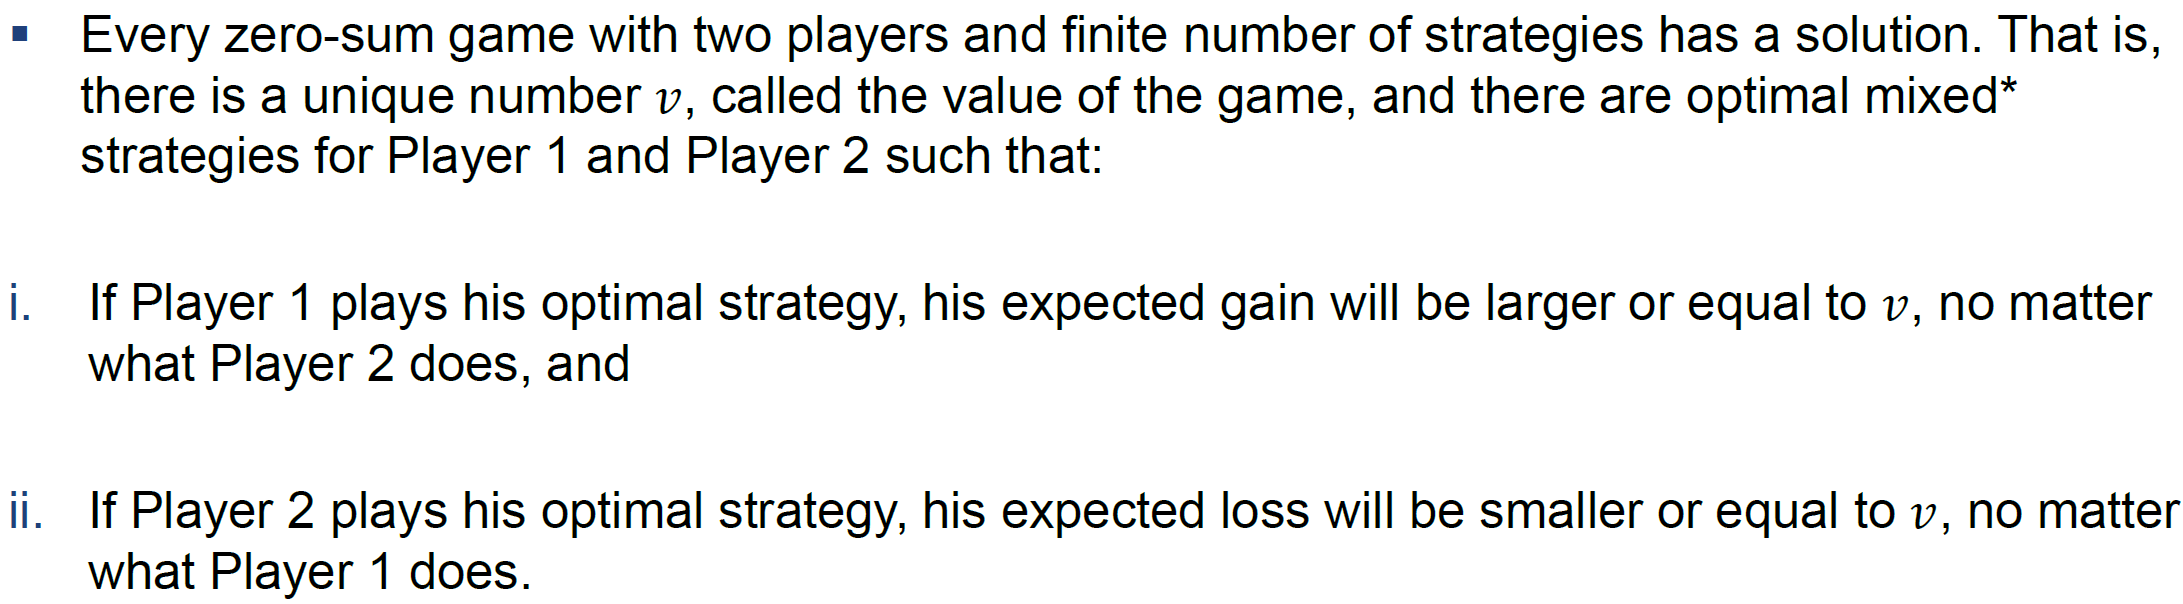
\includegraphics[width=0.5\textwidth]{Pictures/maxmin_theorem.png}
\end{figure}

Comments:
\begin{itemize}
    \item Game Theory began with studies of zero-sum games
    \item In zero-sum (also called constant sum) games:
        \begin{itemize}
            \item The sum of payoffs in each cell is zero (or constant)
            \item The interests of the players are strictly opposite
        \end{itemize}
    \item Maxmin strategy enables a player to calculate the maximum of the minimum
        payoff he can achieve. This strategy guarantees him a security level -
        the minimum payoff for a player, when he plays non-cooperative.
\end{itemize}

Example 10: 2 players, 4 strategies:

\begin{figure}[H]
    \centering
    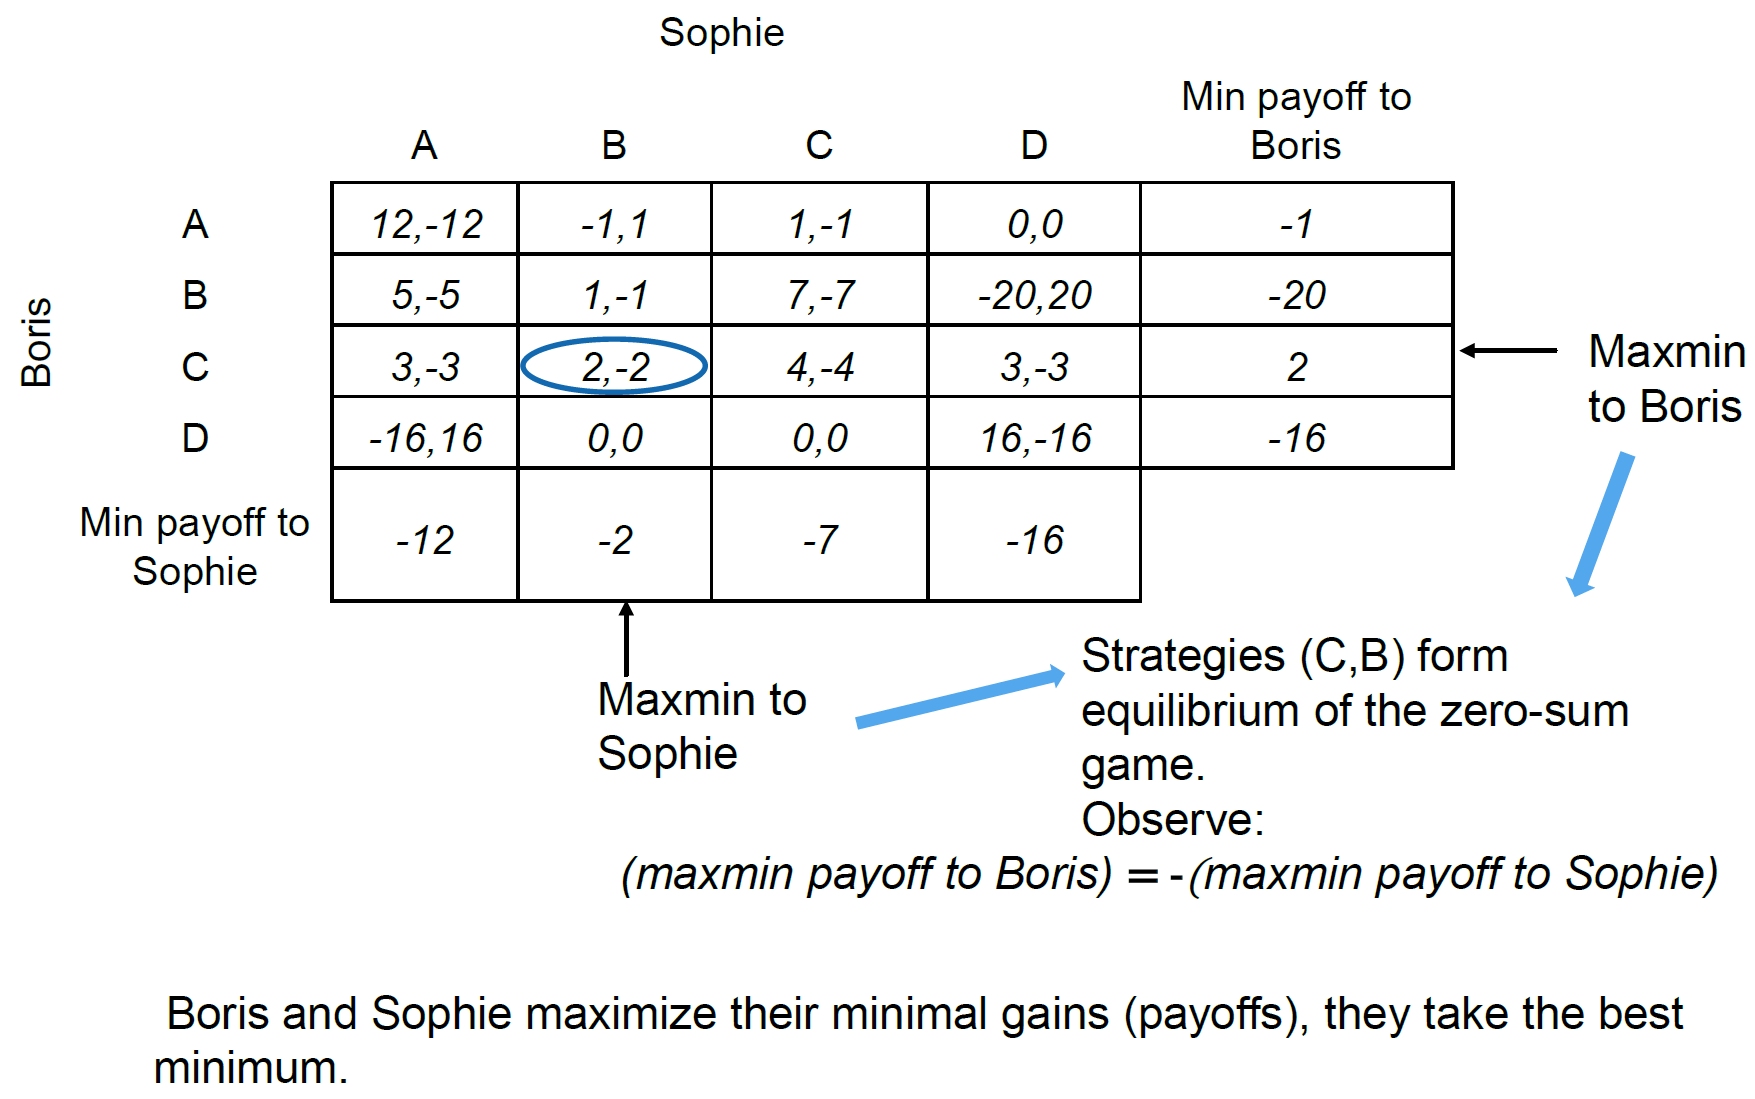
\includegraphics[width=0.5\textwidth]{Pictures/example_10.png}
    \caption{Solution with maxmin}
\end{figure}

\begin{figure}[H]
    \centering
    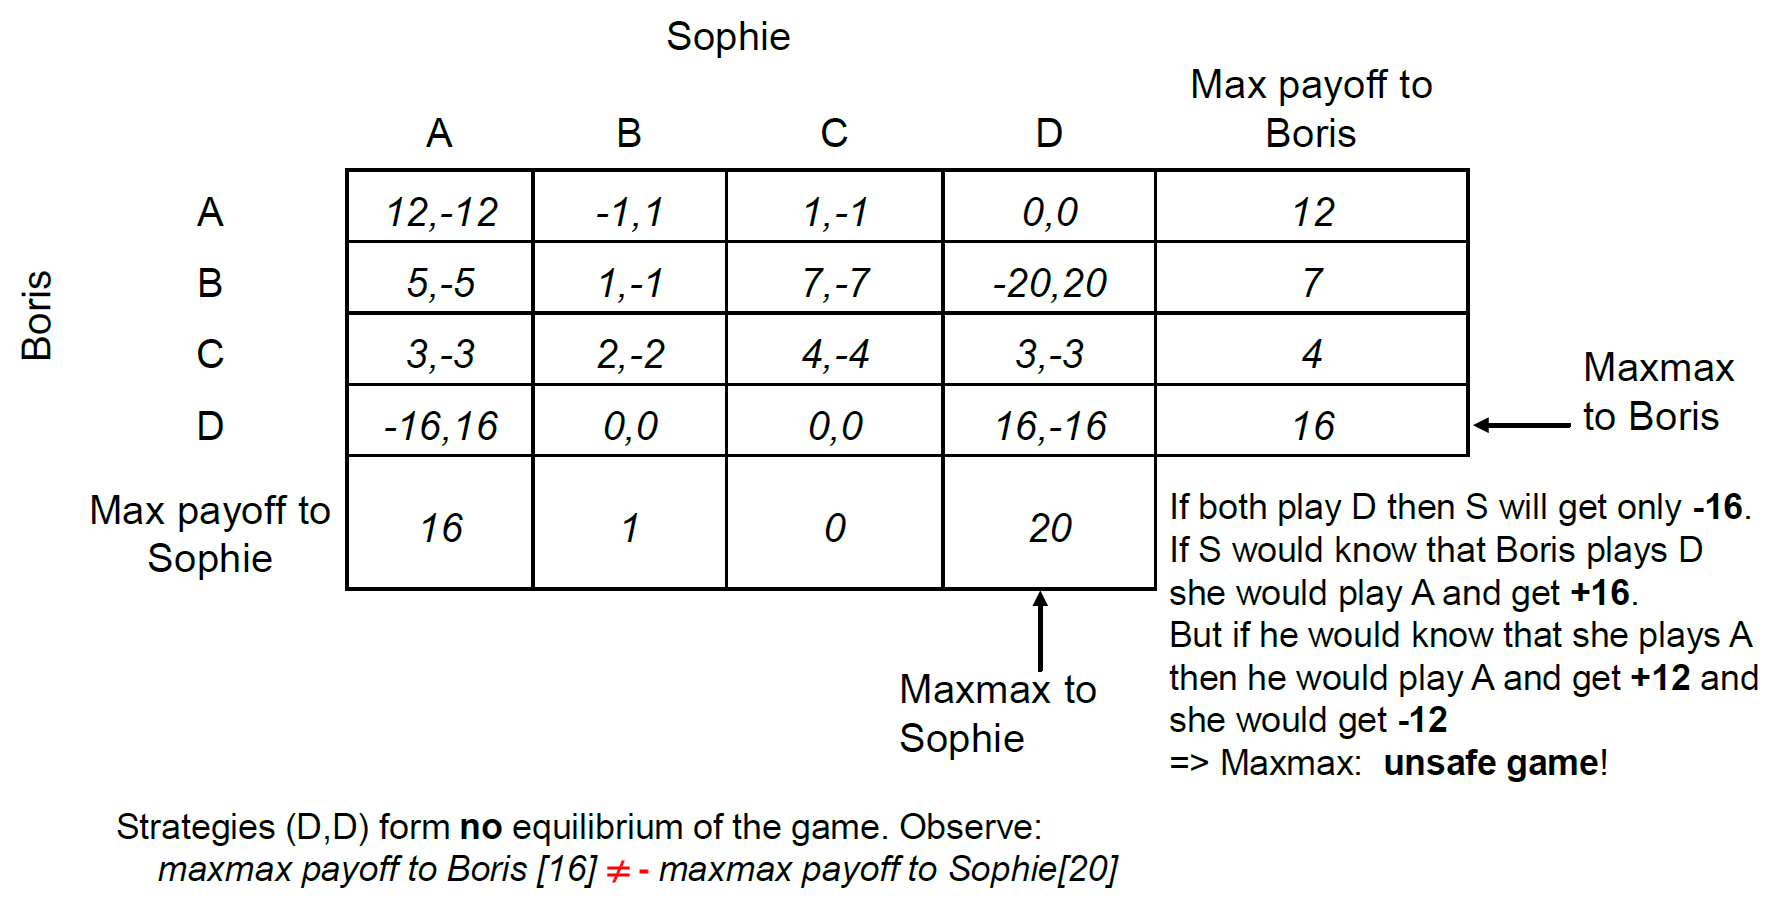
\includegraphics[width=0.5\textwidth]{Pictures/example_10_maxmax.png}
    \caption{Solution with maxmax}
\end{figure}

\begin{figure}[H]
    \centering
    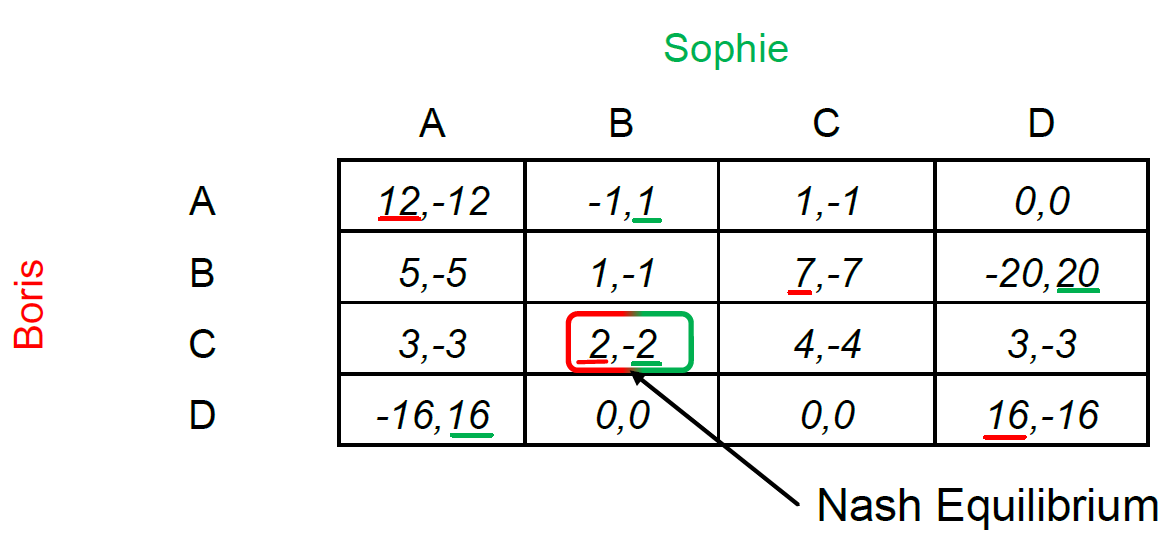
\includegraphics[width=0.5\textwidth]{Pictures/example_10_best_response.png}
    \caption{Solution with the best response / Nash equilibrium}
\end{figure}

\underline{Nash Equilibrium}

\begin{figure}[H]
    \centering
    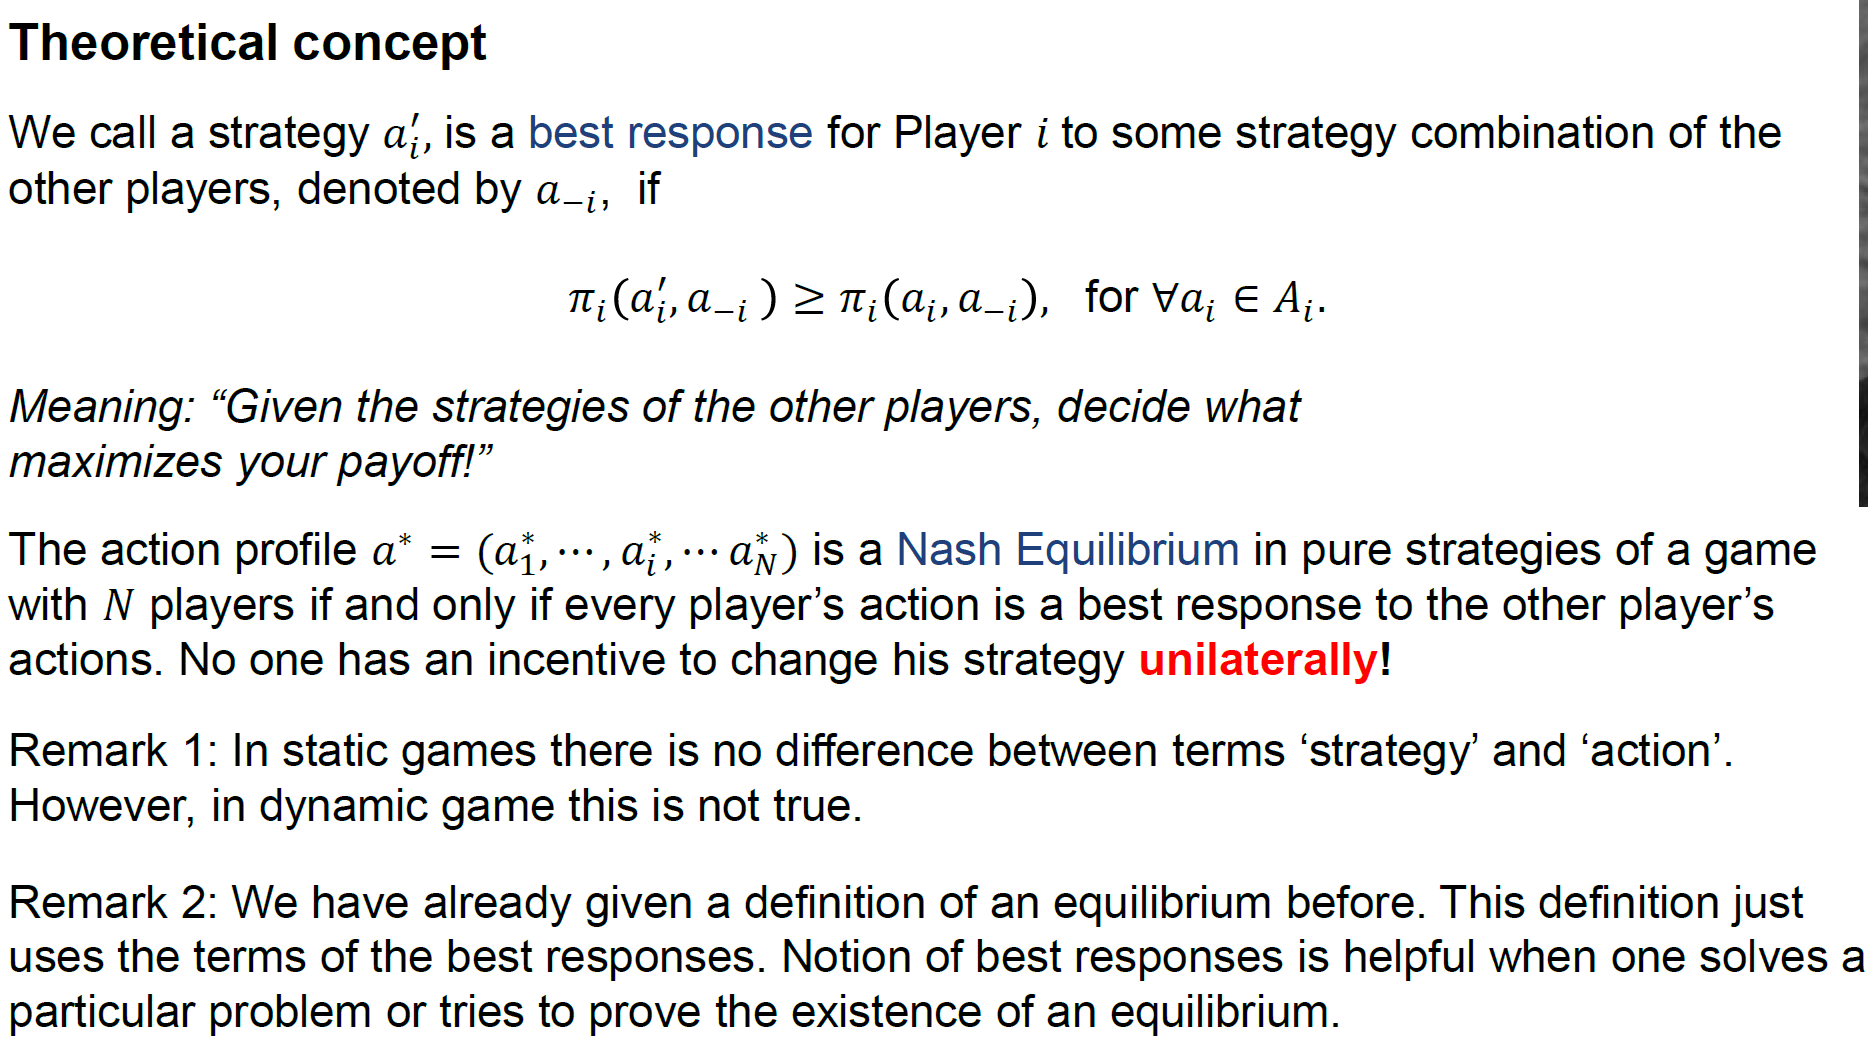
\includegraphics[width=0.6\textwidth]{Pictures/nash_equilibrium.png}
\end{figure}

Comments:
\begin{itemize}
    \item We applied two solution concepts $A$ and $B$: Maxmin by von Neumann
        and Nash Equilibrium.
    \item Both concepts let to the same solution.
    \item The maxmin cocept was developed first and is applicable to constant
        sum games.
    \item Nash's best response is more widely applicable and we will use it from
        now on.
\end{itemize}

Example 11: Equilibrium in pure strategies.

\begin{figure}[H]
    \centering
    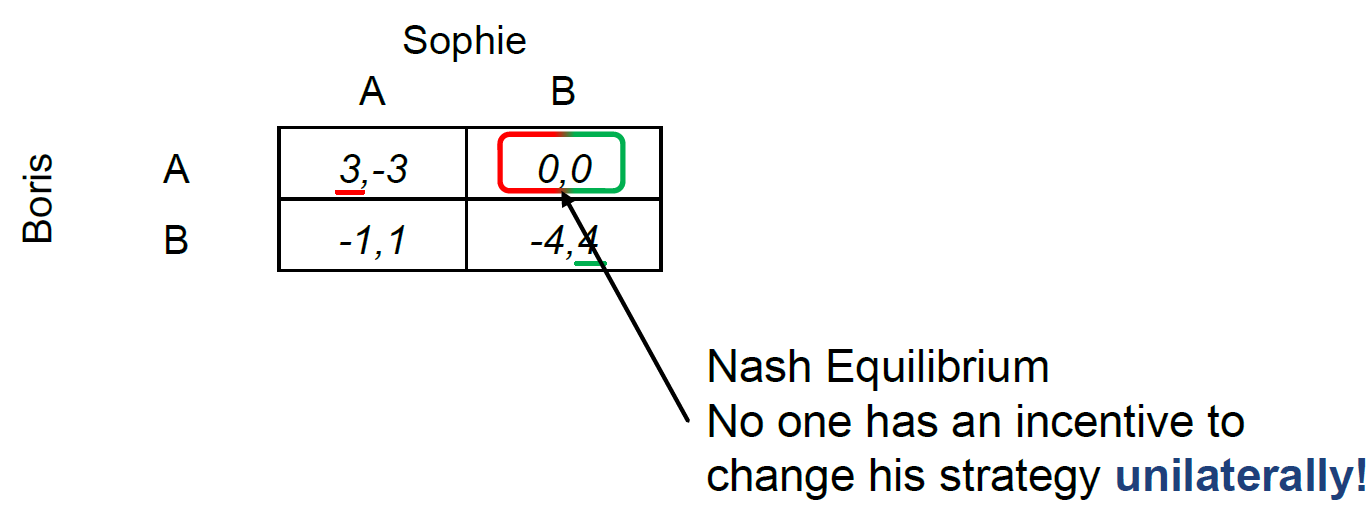
\includegraphics[width=0.5\textwidth]{Pictures/nash_equilibrium_2.png}
\end{figure}

Example 12: No equilibrium in pure strategies.

\begin{figure}[H]
    \centering
    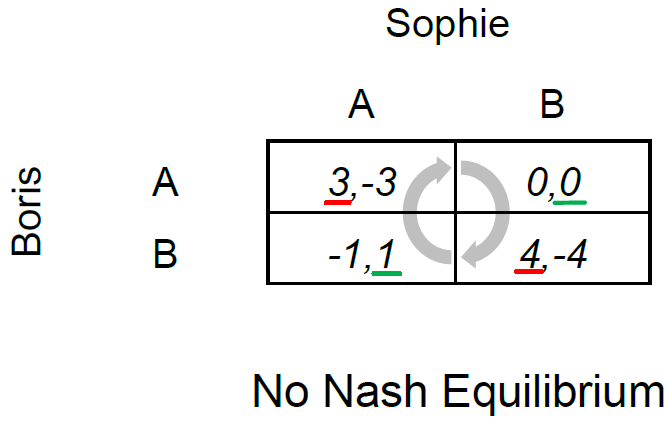
\includegraphics[width=0.4\textwidth]{Pictures/no_nash_equilibrium.png}
\end{figure}

\begin{figure}[H]
    \centering
    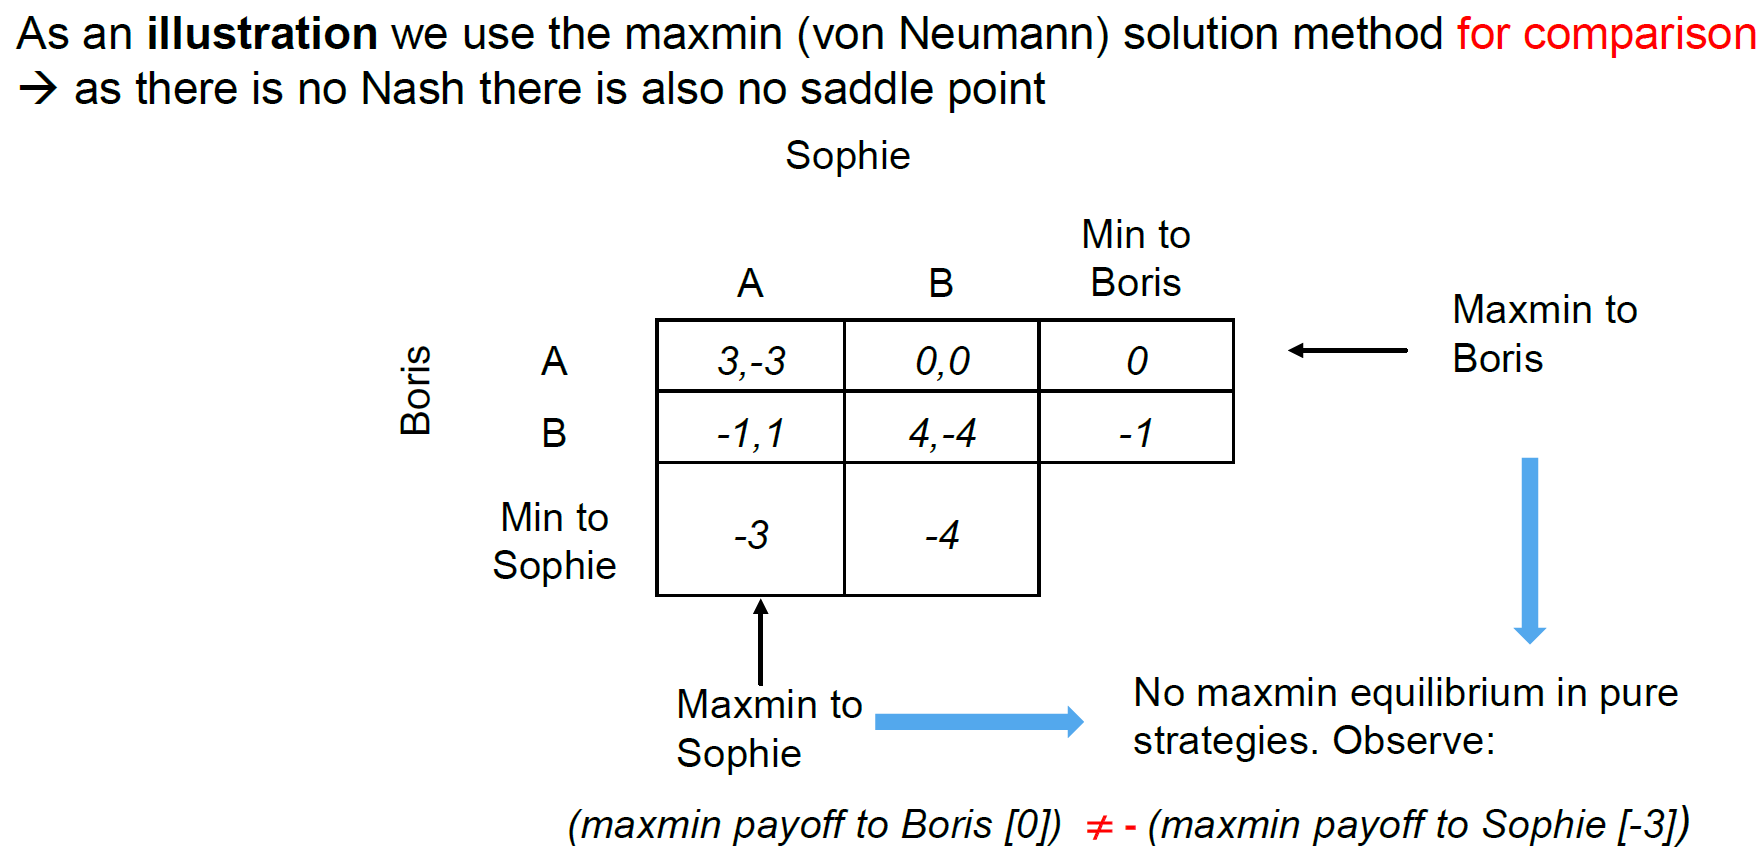
\includegraphics[width=0.6\textwidth]{Pictures/example_12_comment.png}
\end{figure}


Mixed Strategy:

\begin{itemize}
    \item A mixed Strategy specifies the probability with which each of the
        pure strategies is used.
    \item Example: Suppose the set of pure strategies to player $i$ is $S_i = \geschwungeneklammer{s_a,s_b,\dots}$
        Then the mixed strategy is a vector of probabilities
        $\sigma_i = \klammer{p(s_a) , p(s_b) , p(s_c) , \dots}$ such that
        $\sum_{s \in S_i} p(s) = 1$
    \item A pure strategy can pe represented as a special case of a mixed strategy.
\end{itemize}

Back to example 12:

\begin{figure}[H]
    \centering
    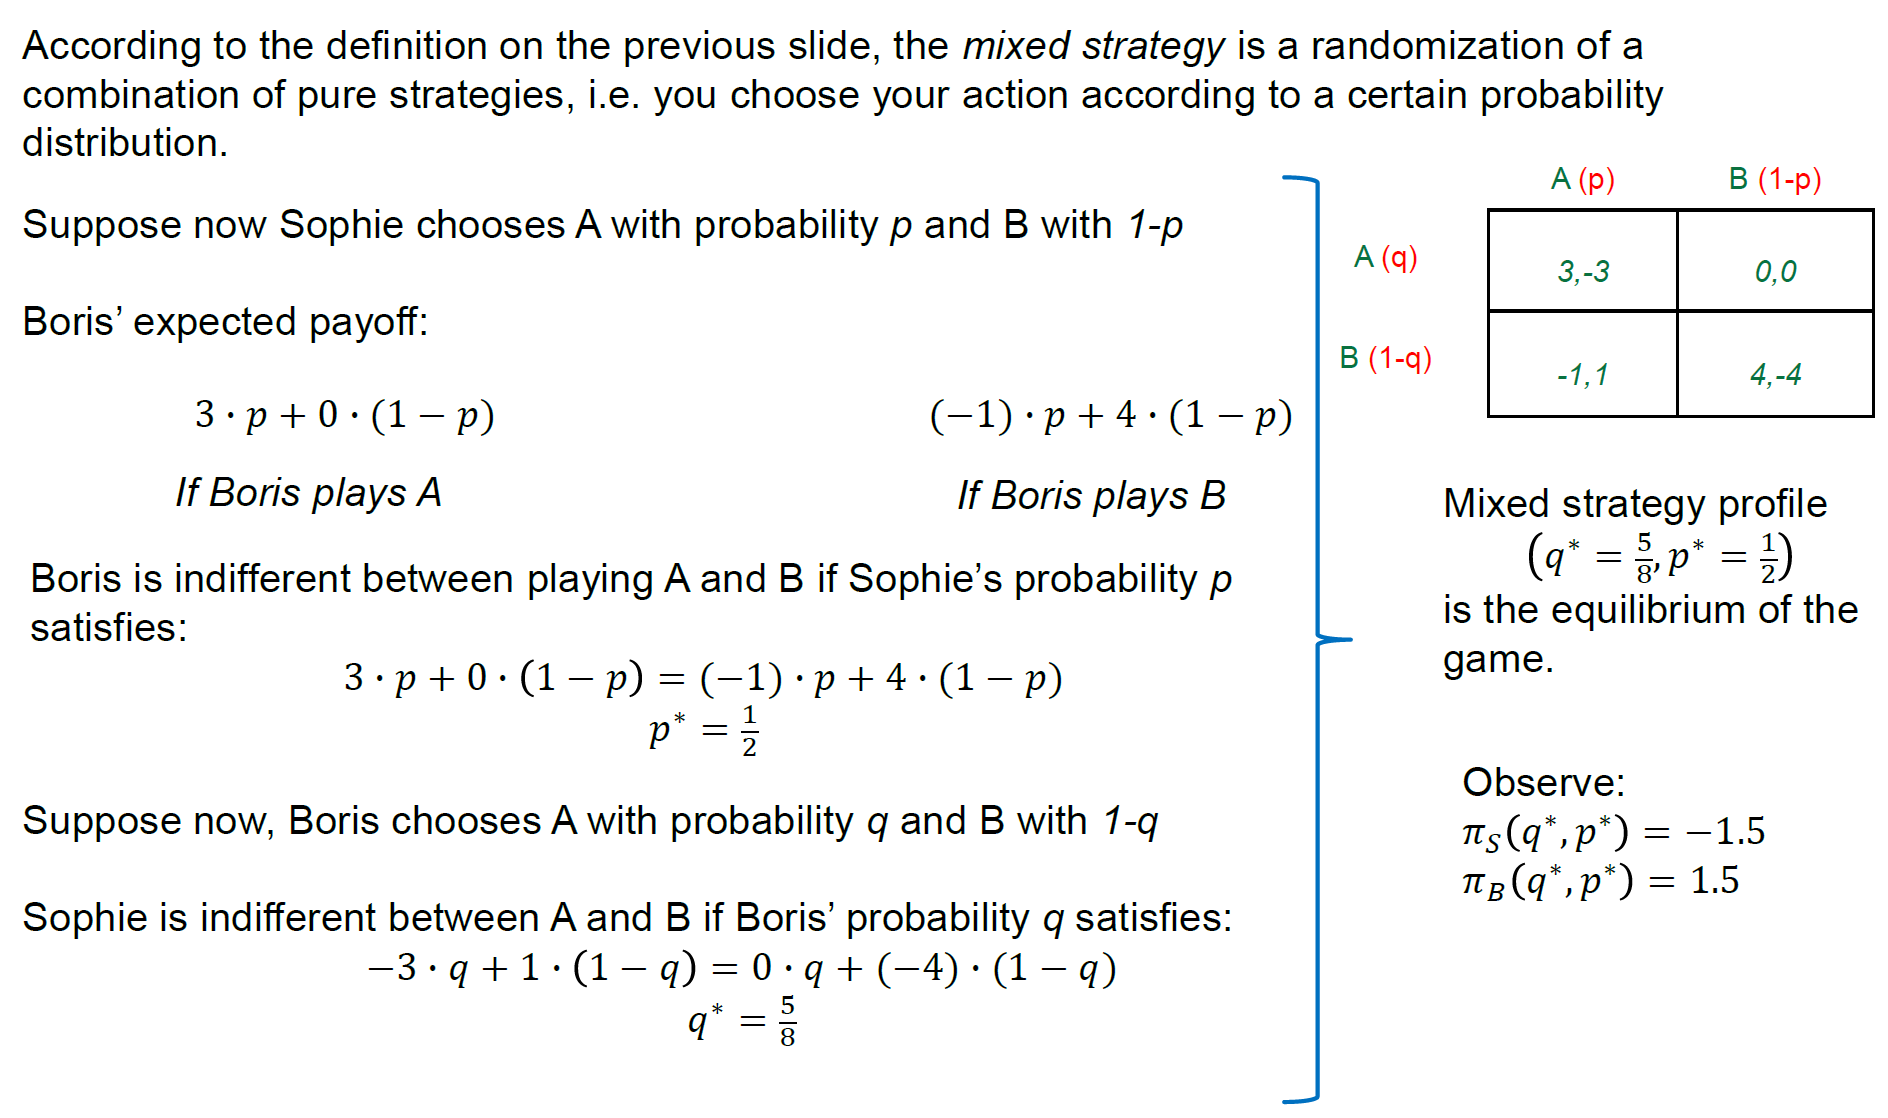
\includegraphics[width=0.7\textwidth]{Pictures/example_12_mixed_strategy.png}
\end{figure}

\subparagraph{Non constant sum game}

Example 13: Maroni game

\begin{figure}[H]
    \centering
    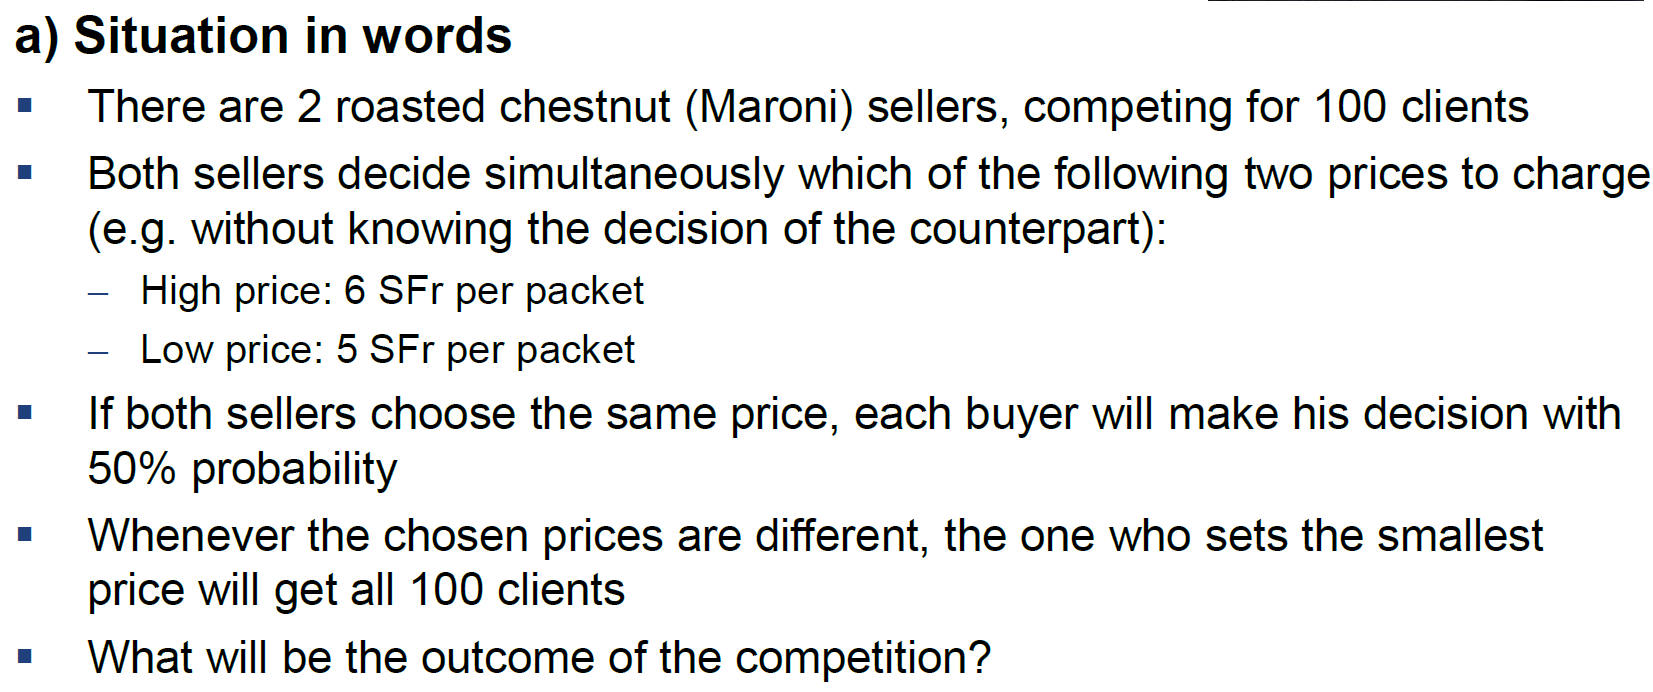
\includegraphics[width=0.6\textwidth]{Pictures/maroni1.png}
    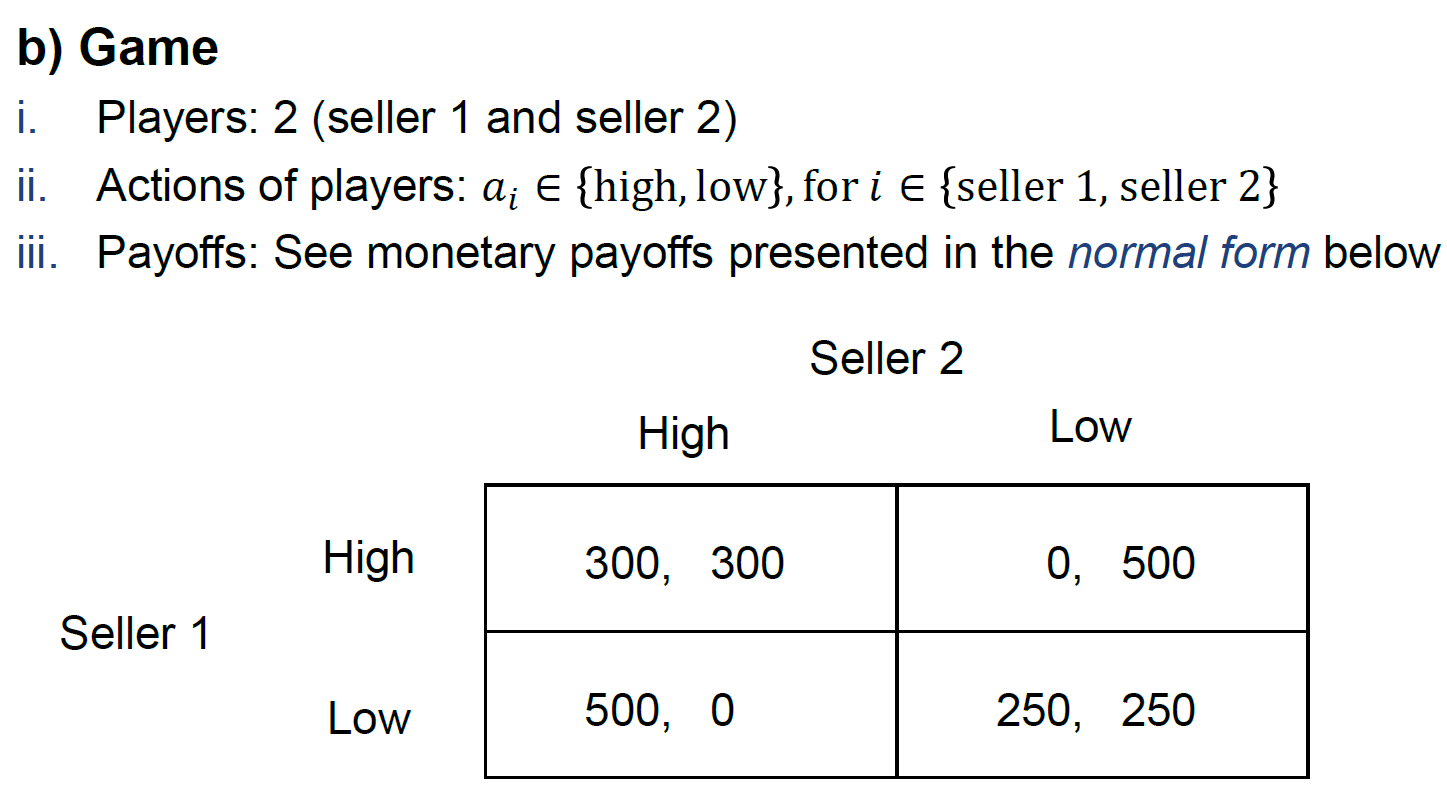
\includegraphics[width=0.6\textwidth]{Pictures/maroni2.png}
\end{figure}
Nash equilibrium at 250,250.

\begin{figure}[H]
    \centering
    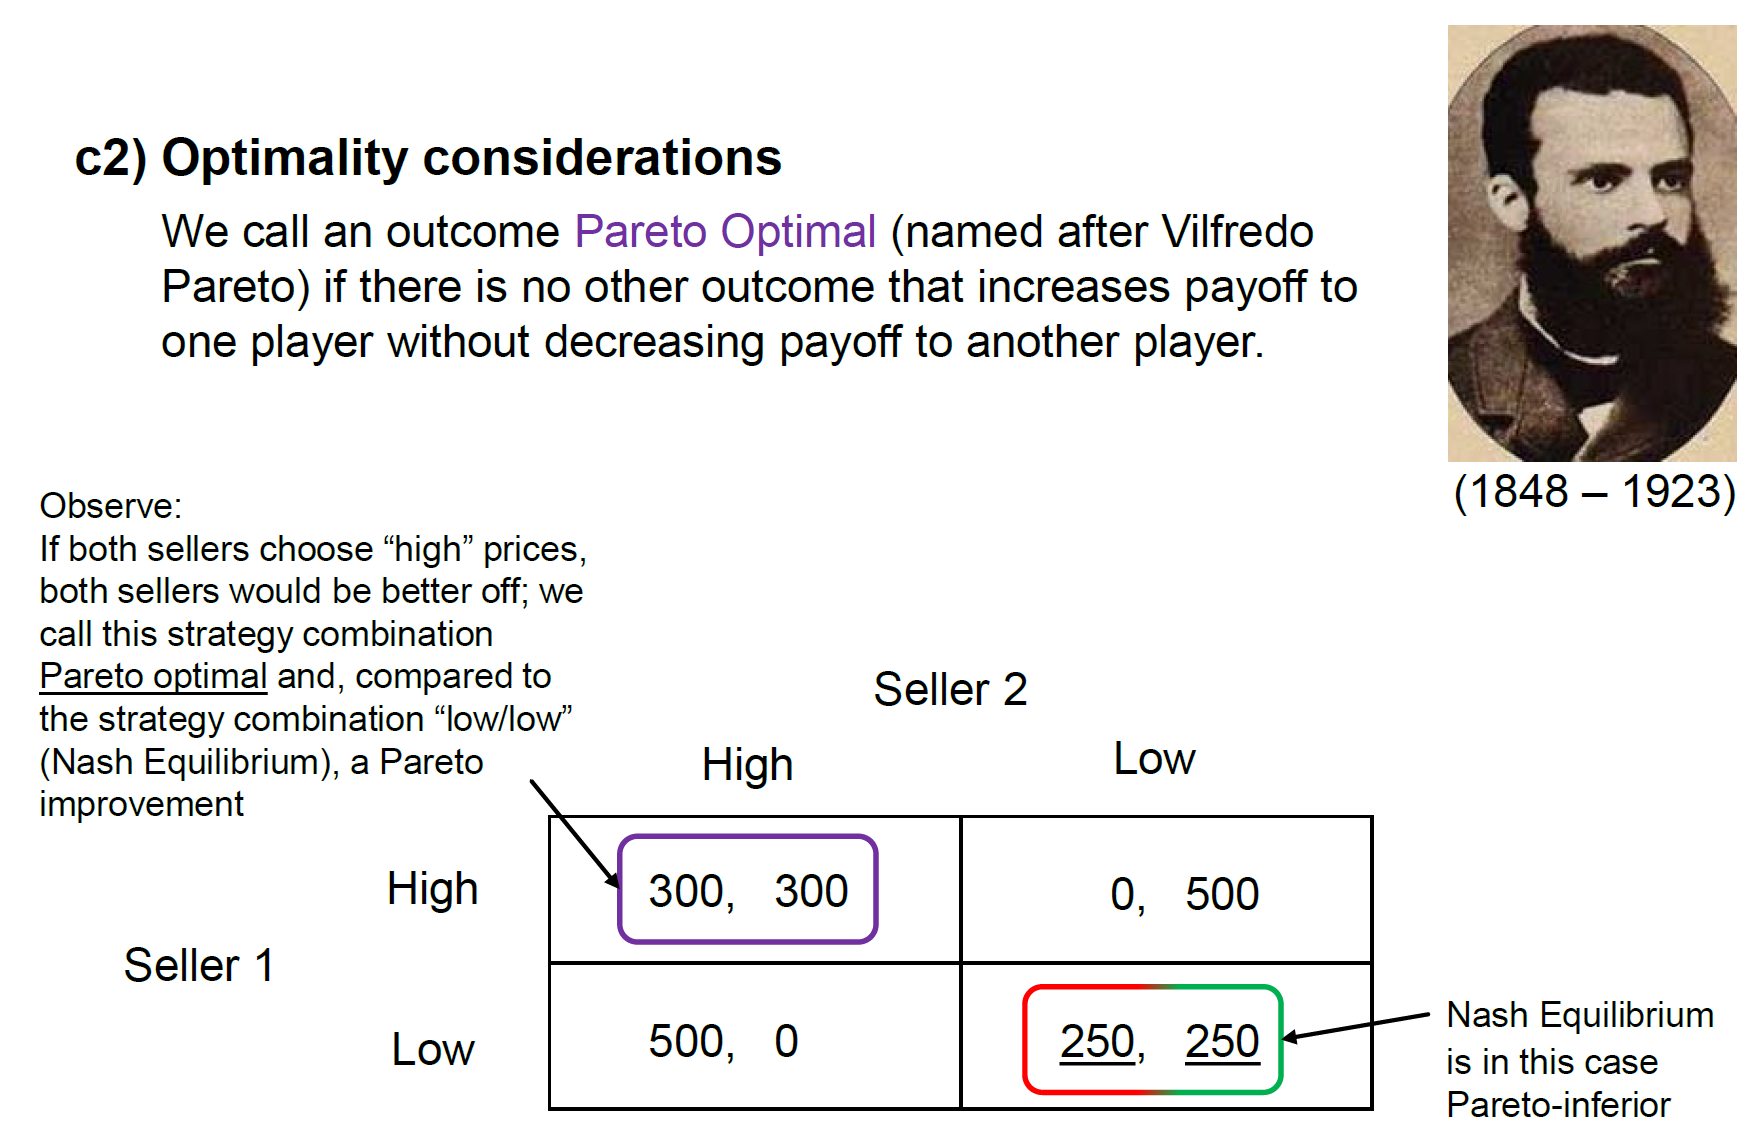
\includegraphics[width=0.5\textwidth]{Pictures/maroni3.png}
\end{figure}
"Low" is the dominant strategy.

\vspace{1\baselineskip}

Comments:
\begin{itemize}
    \item Game illustrates conflict in "economics"
    \item For both sellers strategy "low"-pricing dominates strategy "high"-pricing
    \item Nash Equilibrium is not always Pareto optimal outcome
    \item This is a typical illustration of the Prisoners' Dilemma
\end{itemize}

\vspace{1\baselineskip}

\underline{Classical Prisoners' Dilemma}

\begin{figure}[h]
    \centering
    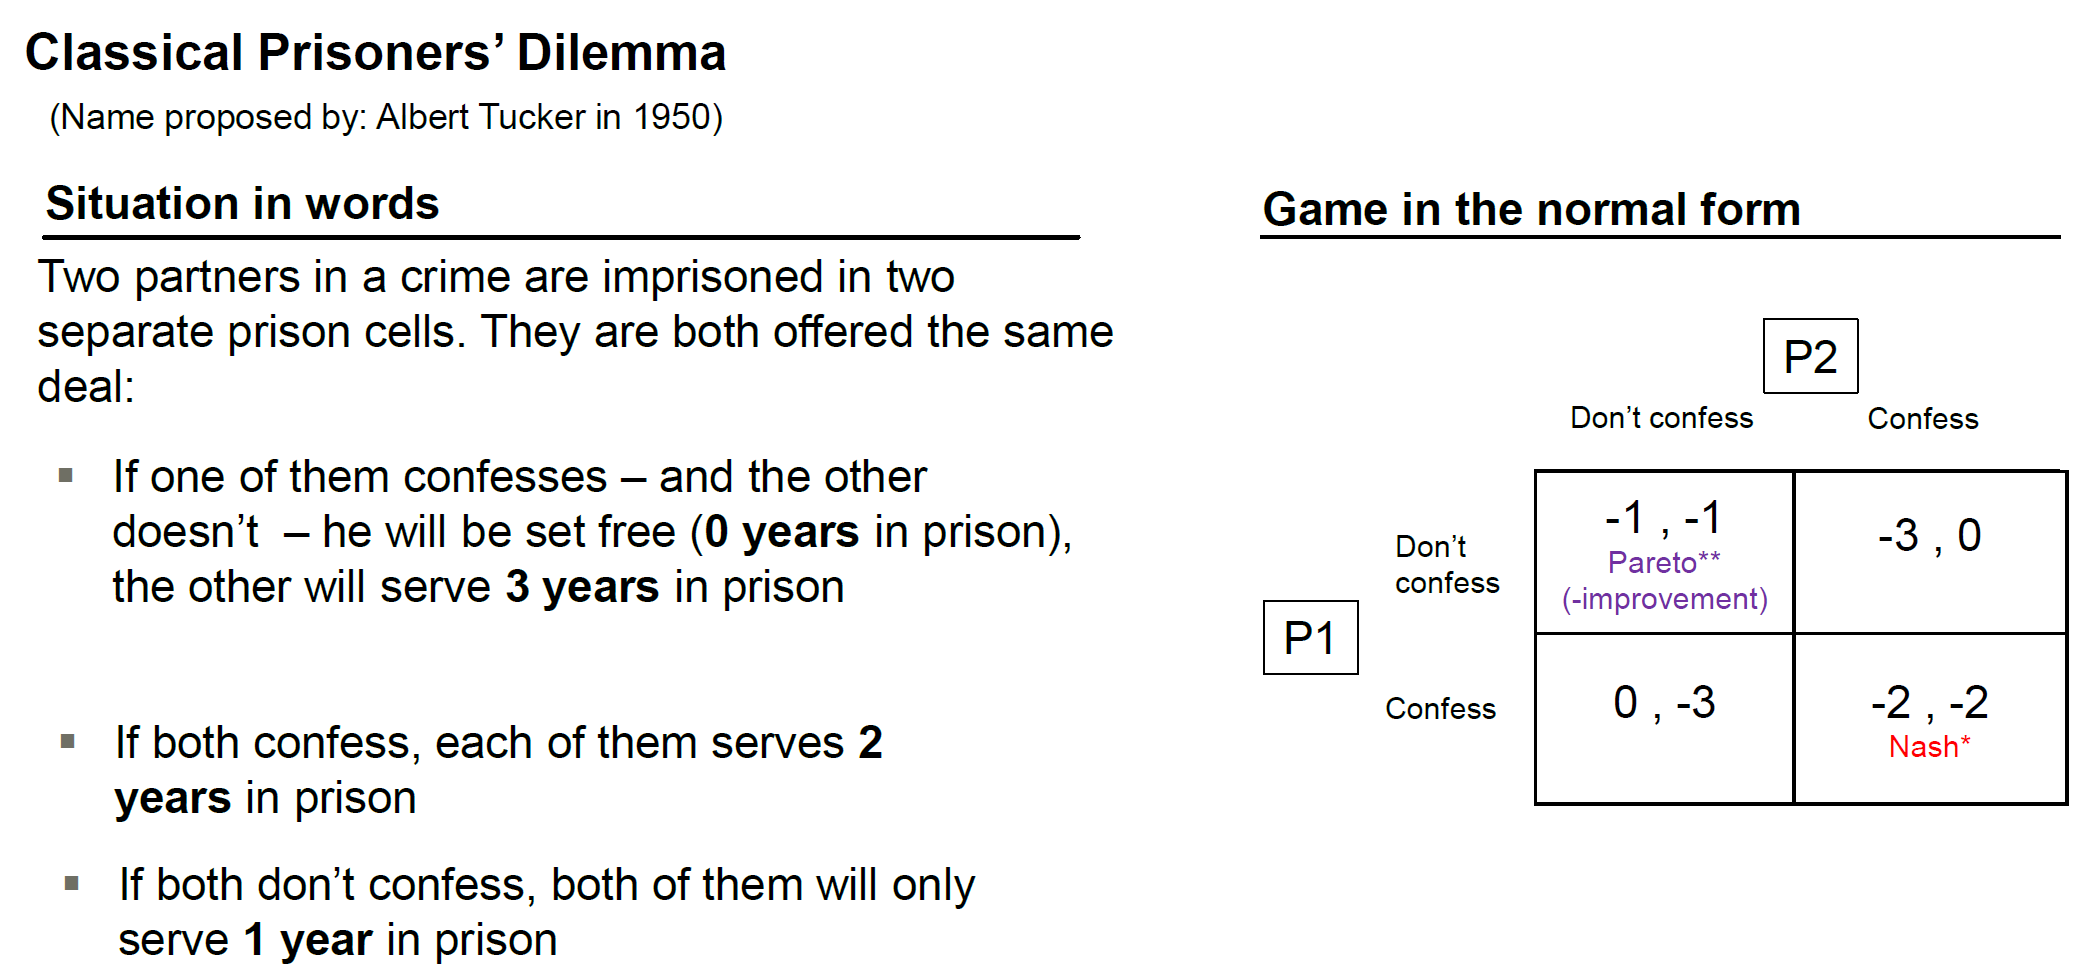
\includegraphics[width=0.7\textwidth]{Pictures/Prisoners_dilemma.png}
\end{figure}

\begin{figure}[H]
    \centering
    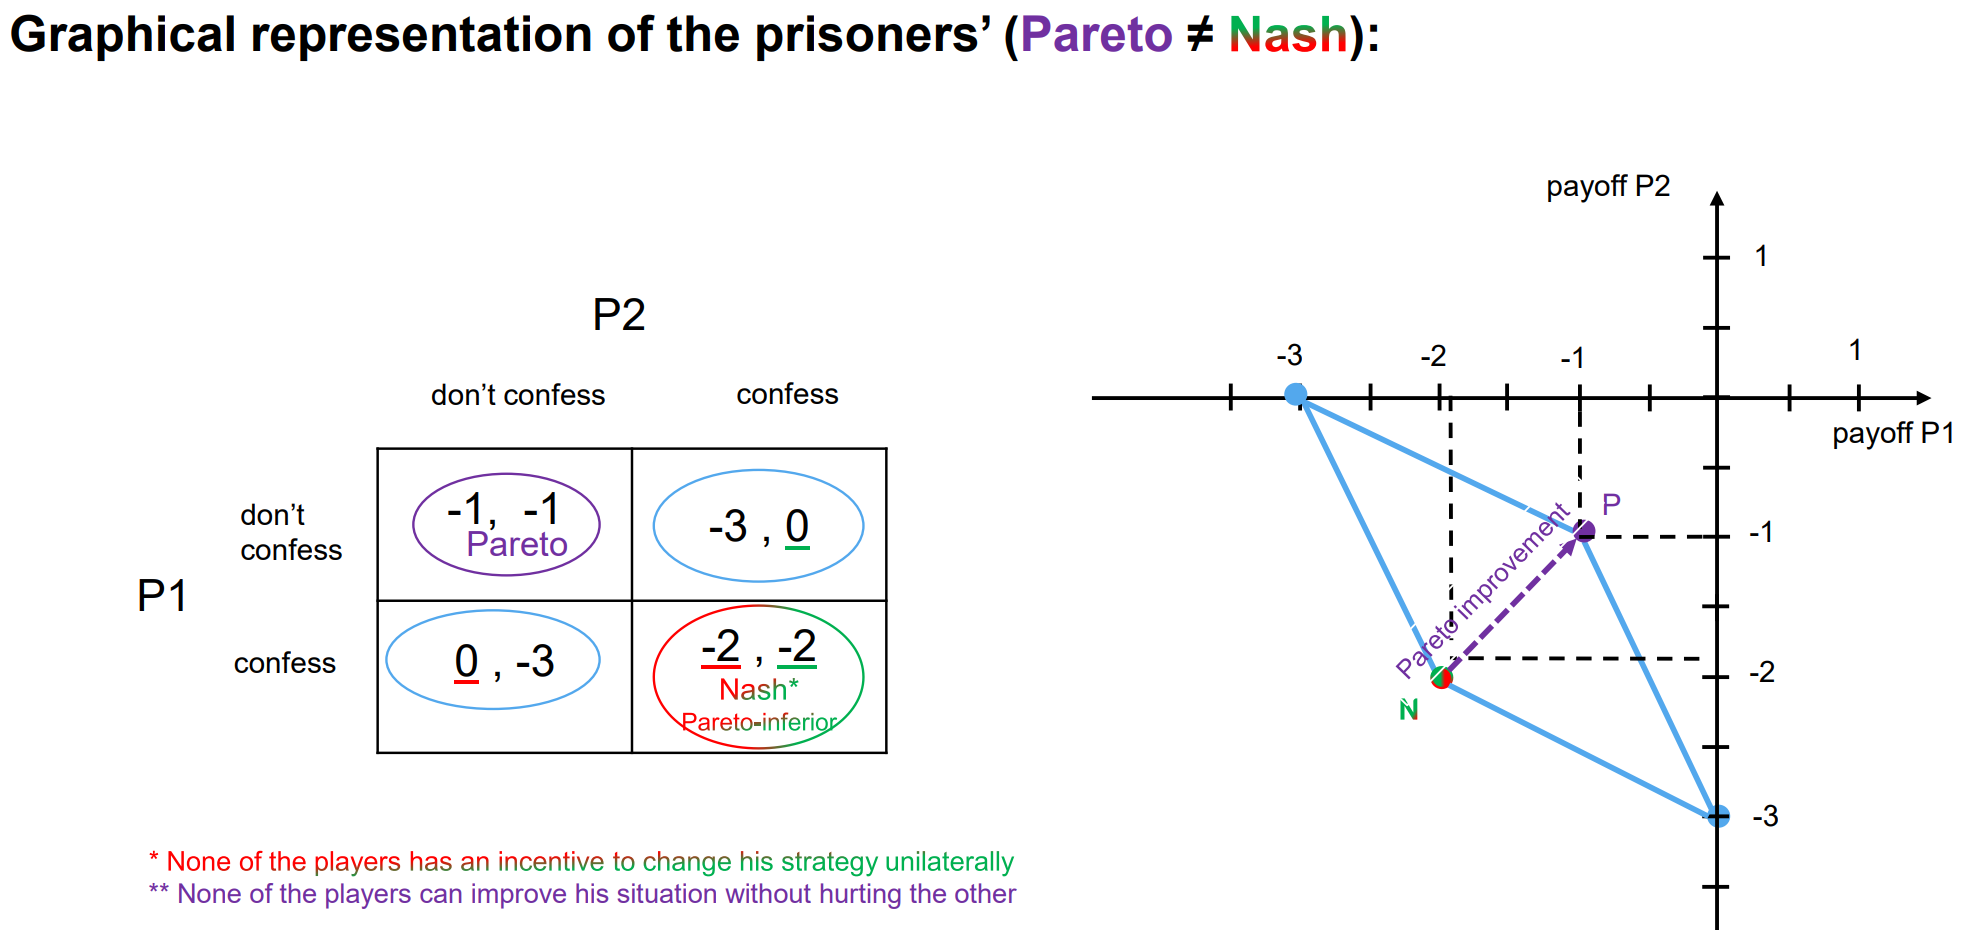
\includegraphics[width=0.8\textwidth]{Pictures/nash_pareto.png}
\end{figure}


\underline{Example 14:}
Situation:
\begin{itemize}
    \item Two countries disagree over the right of a patch of territory.
    \item The governments can decide whether to announce mobilization (and thus
        escalate conflict further) or to refrain from mobilization (and thus
        deescalate the conflict)
    \item When both countries decide to mobilize, the probability of war increases,
        while chances of peace resolution are getting smaller. This is the least
        preferred outcome for both countries as they fall in a devastating war
        (both receive utility of $0$)
    \item Whenever one country mobilizes and the other does not, the mobilizing
        army can get control over the territory without a war. This is the most
        attractive situation for the aggressor (utility of $4$) and the
        refraining country does not incur costs of war (utility of $2$).
    \item When both countries choose to refrain the likelihood of peaceful
        sharing of territory is high (utility of $3$).
\end{itemize}
Game:
\begin{enumerate}[(i)]
    \item Players: 2
    \item Actions of players: mobilize, refrain
    \item Payoffs: Summarized in normal form below:
\end{enumerate}

\begin{figure}[H]
    \centering
    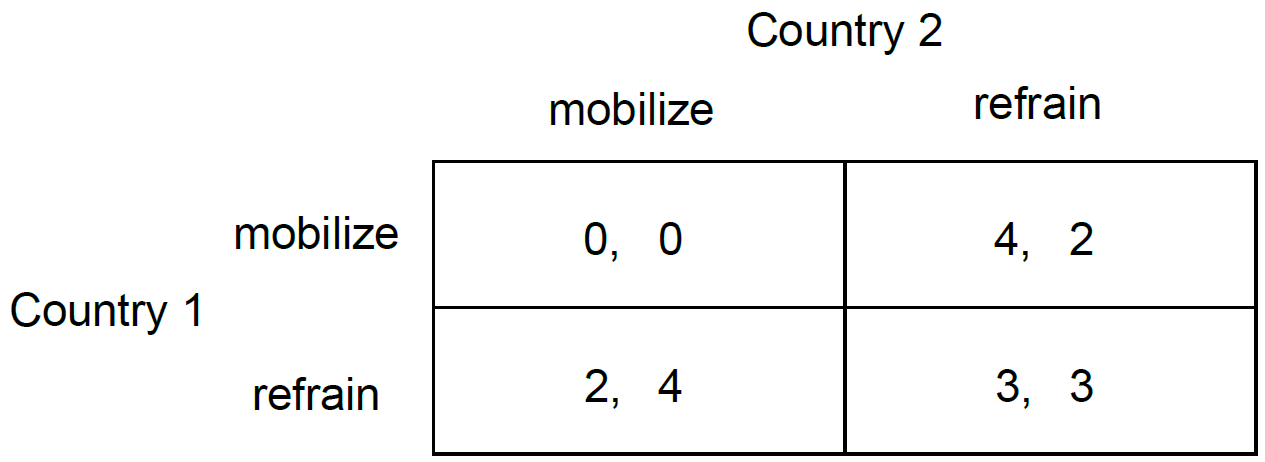
\includegraphics[width=0.5\textwidth]{Pictures/chicken_game.png}
\end{figure}

\begin{figure}[H]
    \centering
    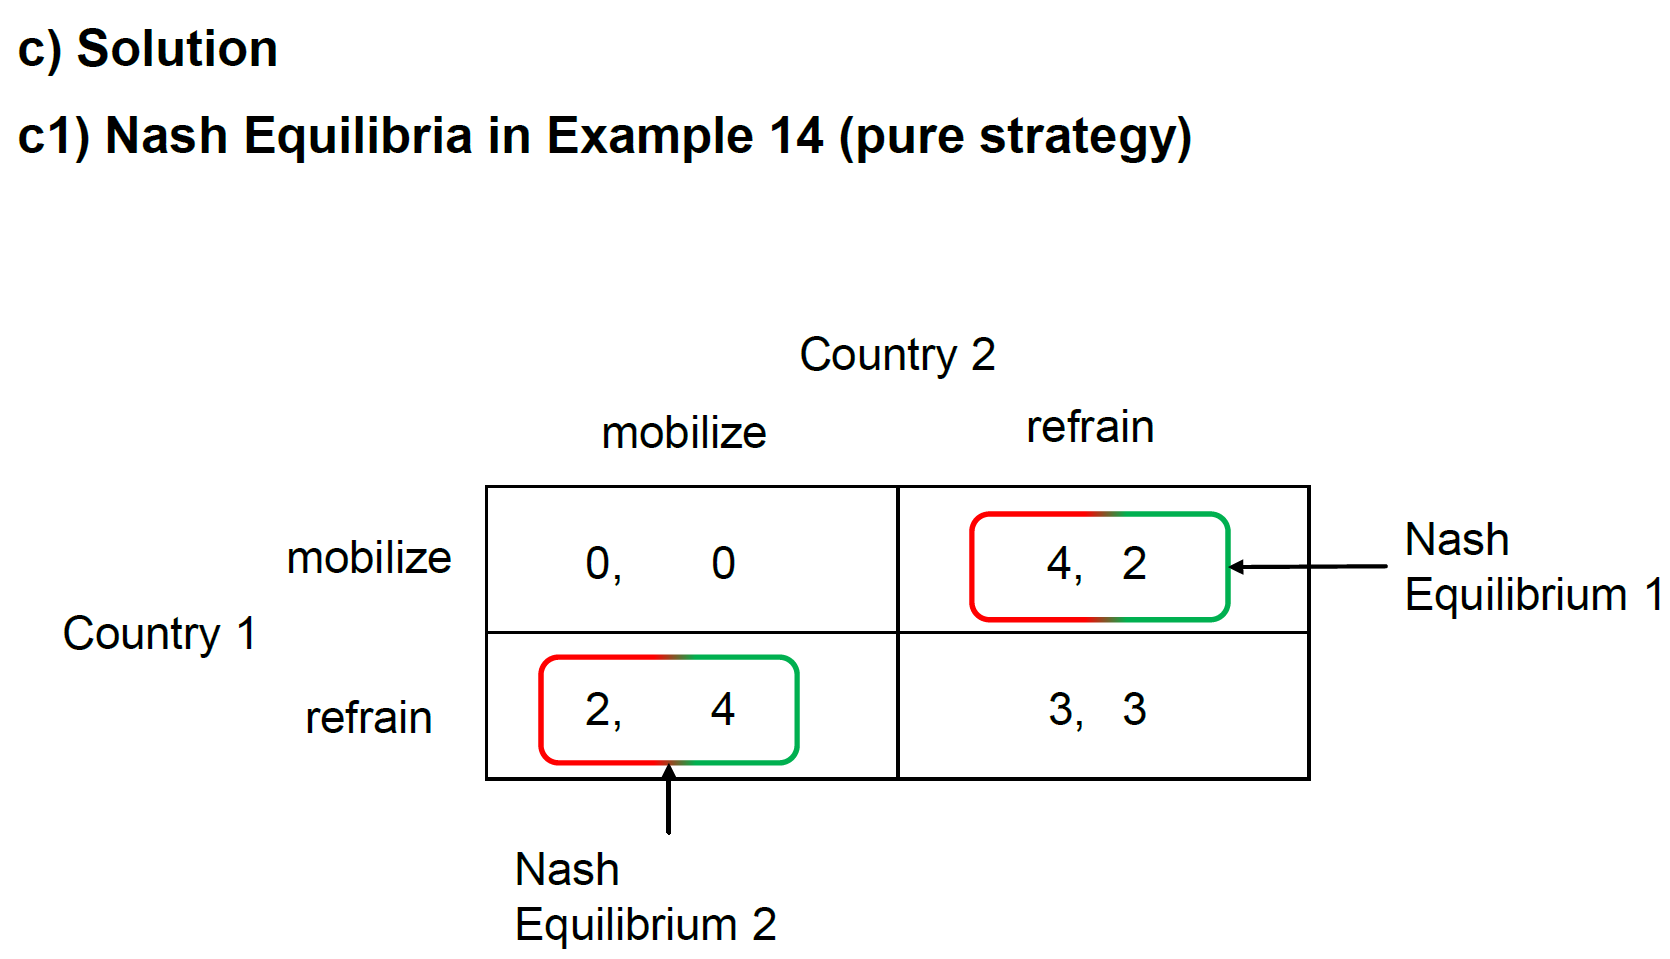
\includegraphics[width=0.5\textwidth]{Pictures/chicken_solution.png}
\end{figure}

\begin{figure}[H]
    \centering
    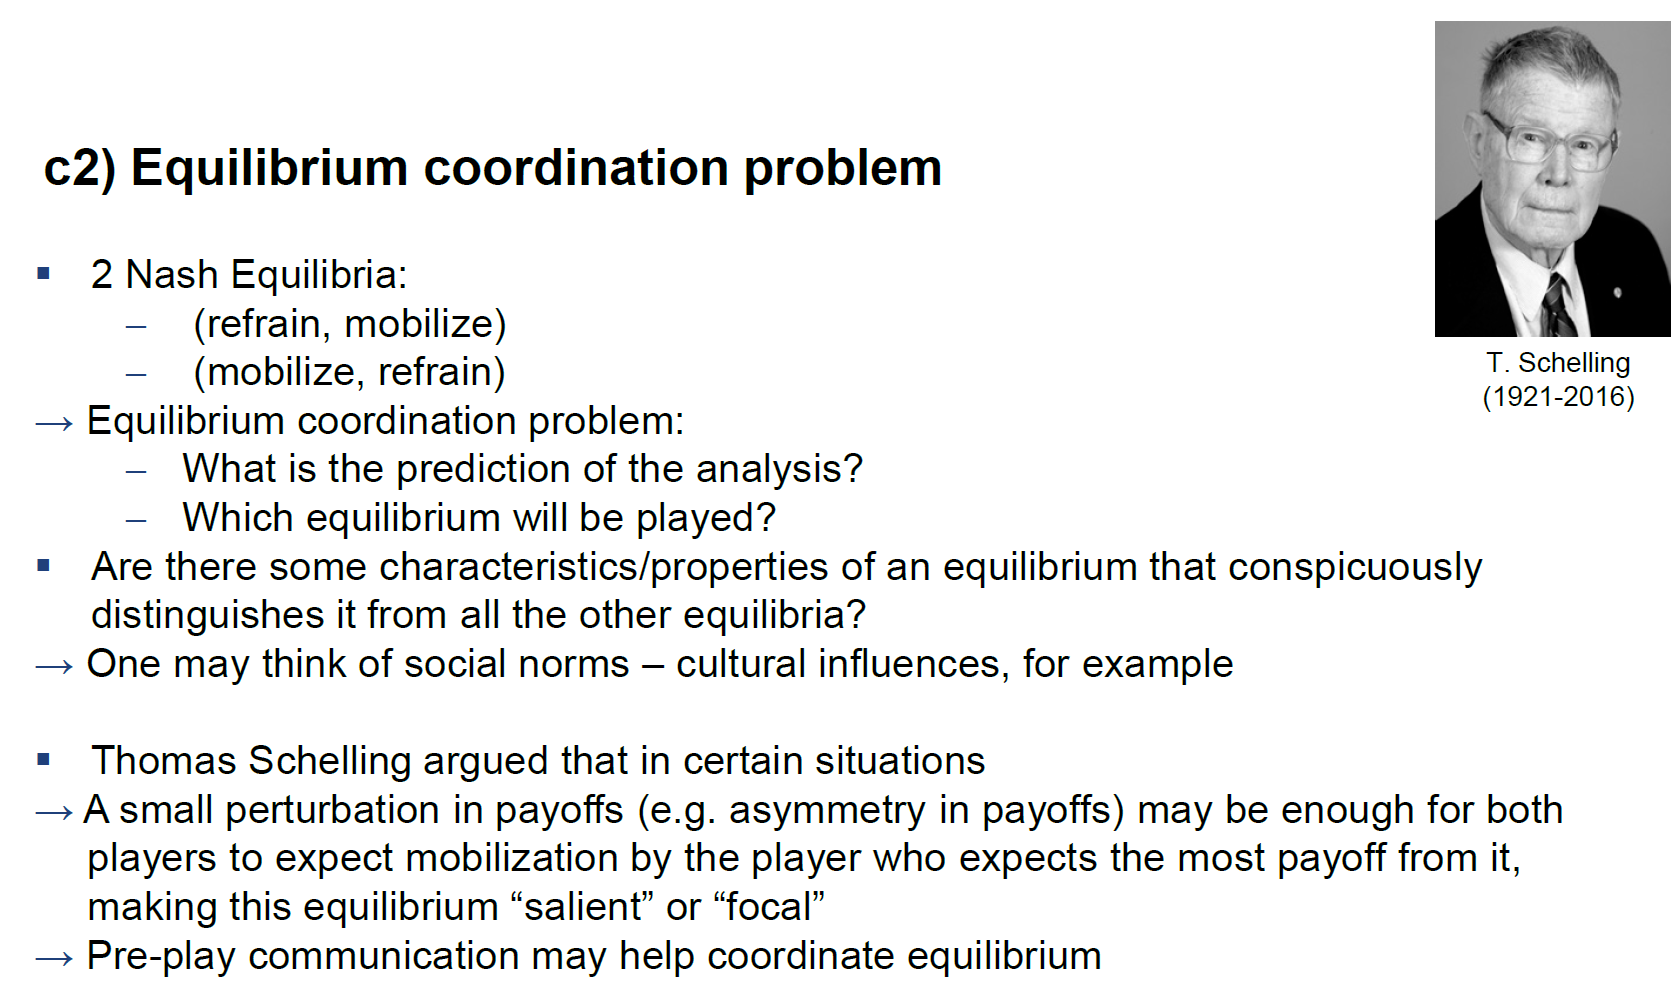
\includegraphics[width=0.7\textwidth]{Pictures/chicken_equilibrium.png}
\end{figure}

\begin{figure}[H]
    \centering
    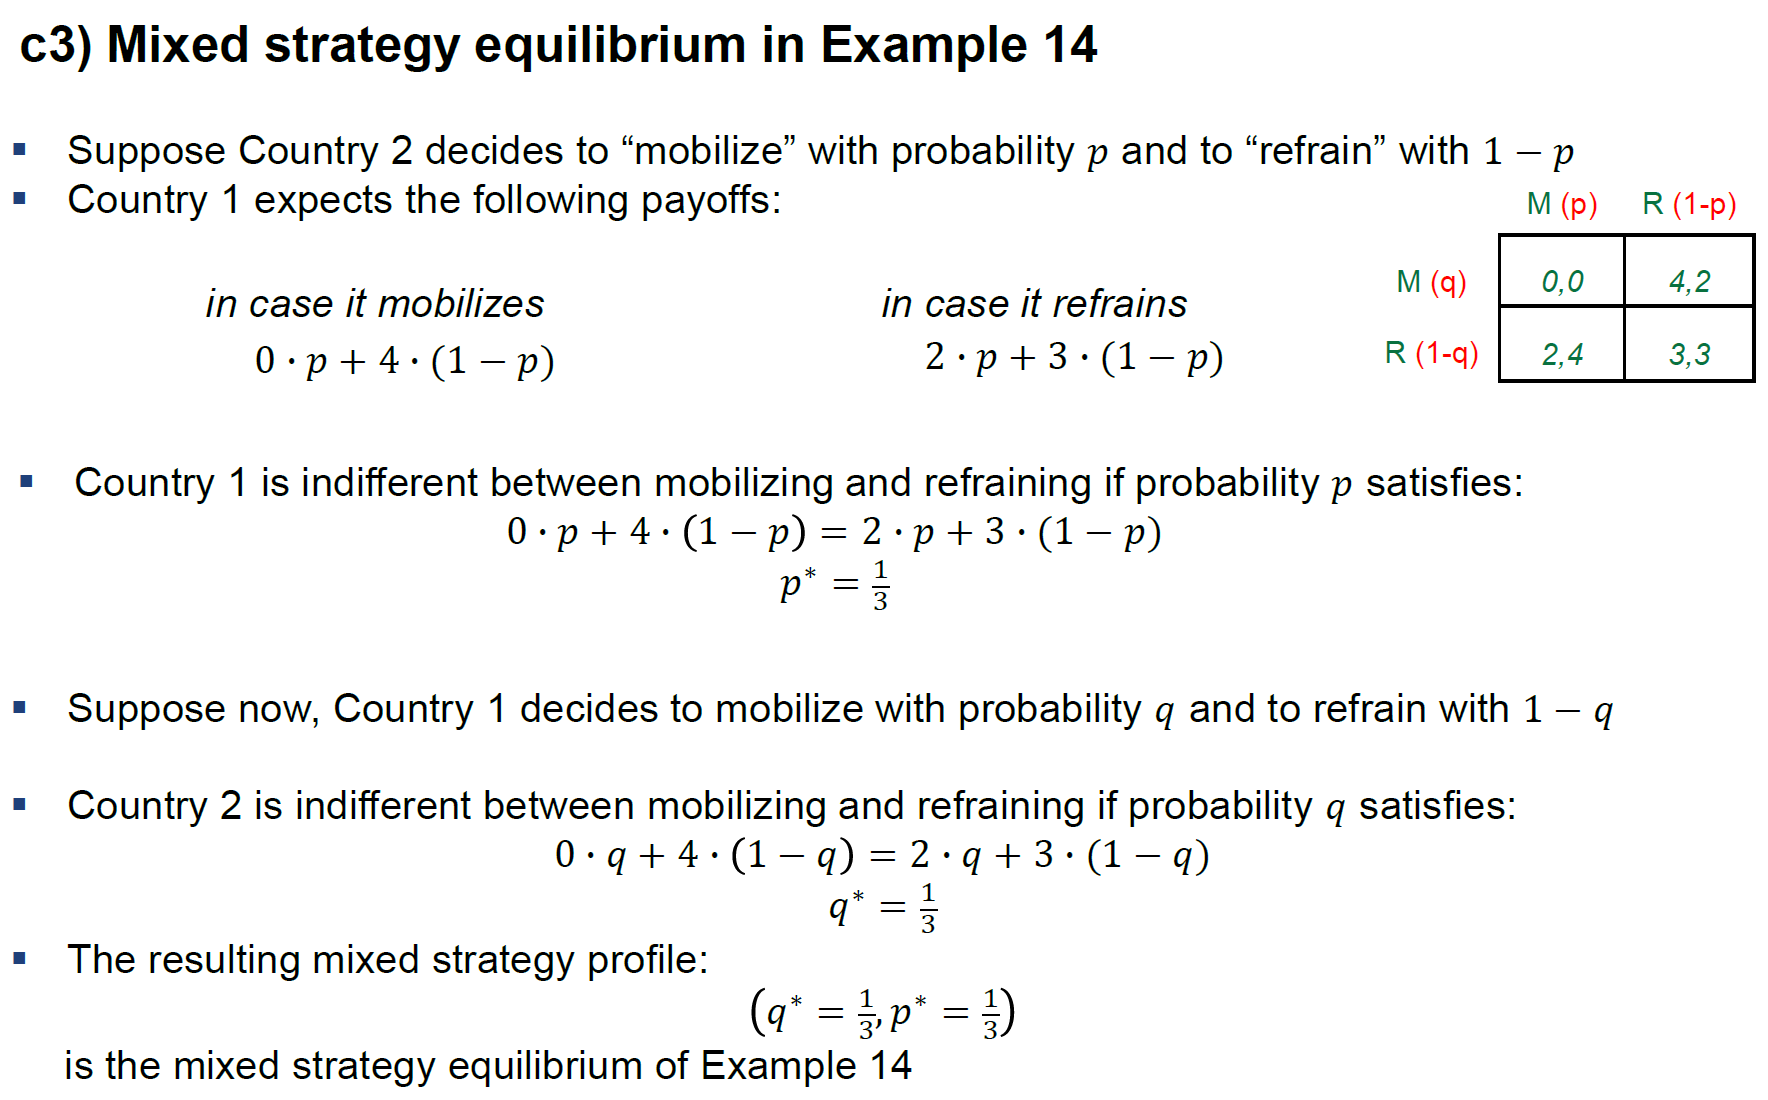
\includegraphics[width=0.6\textwidth]{Pictures/chicken_mixed_strategy.png}
\end{figure}

\begin{figure}[H]
    \centering
    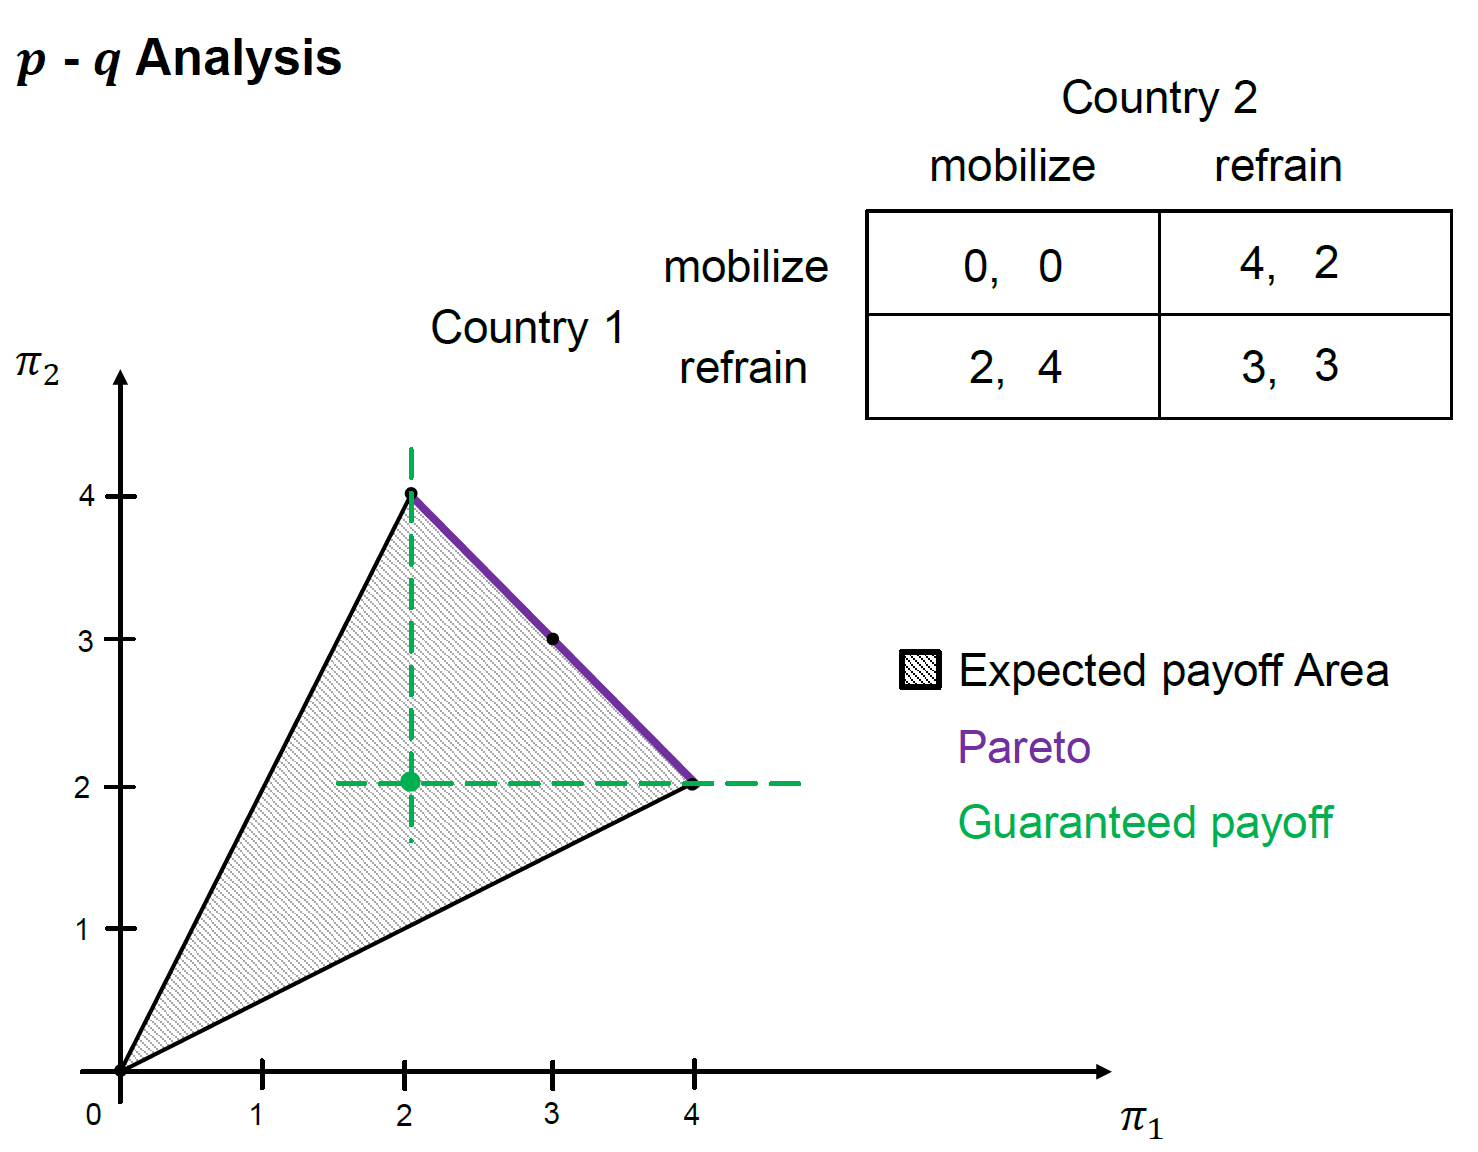
\includegraphics[width=0.5\textwidth]{Pictures/chicken_q_p_analysis.png}
\end{figure}

\begin{figure}[H]
    \centering
    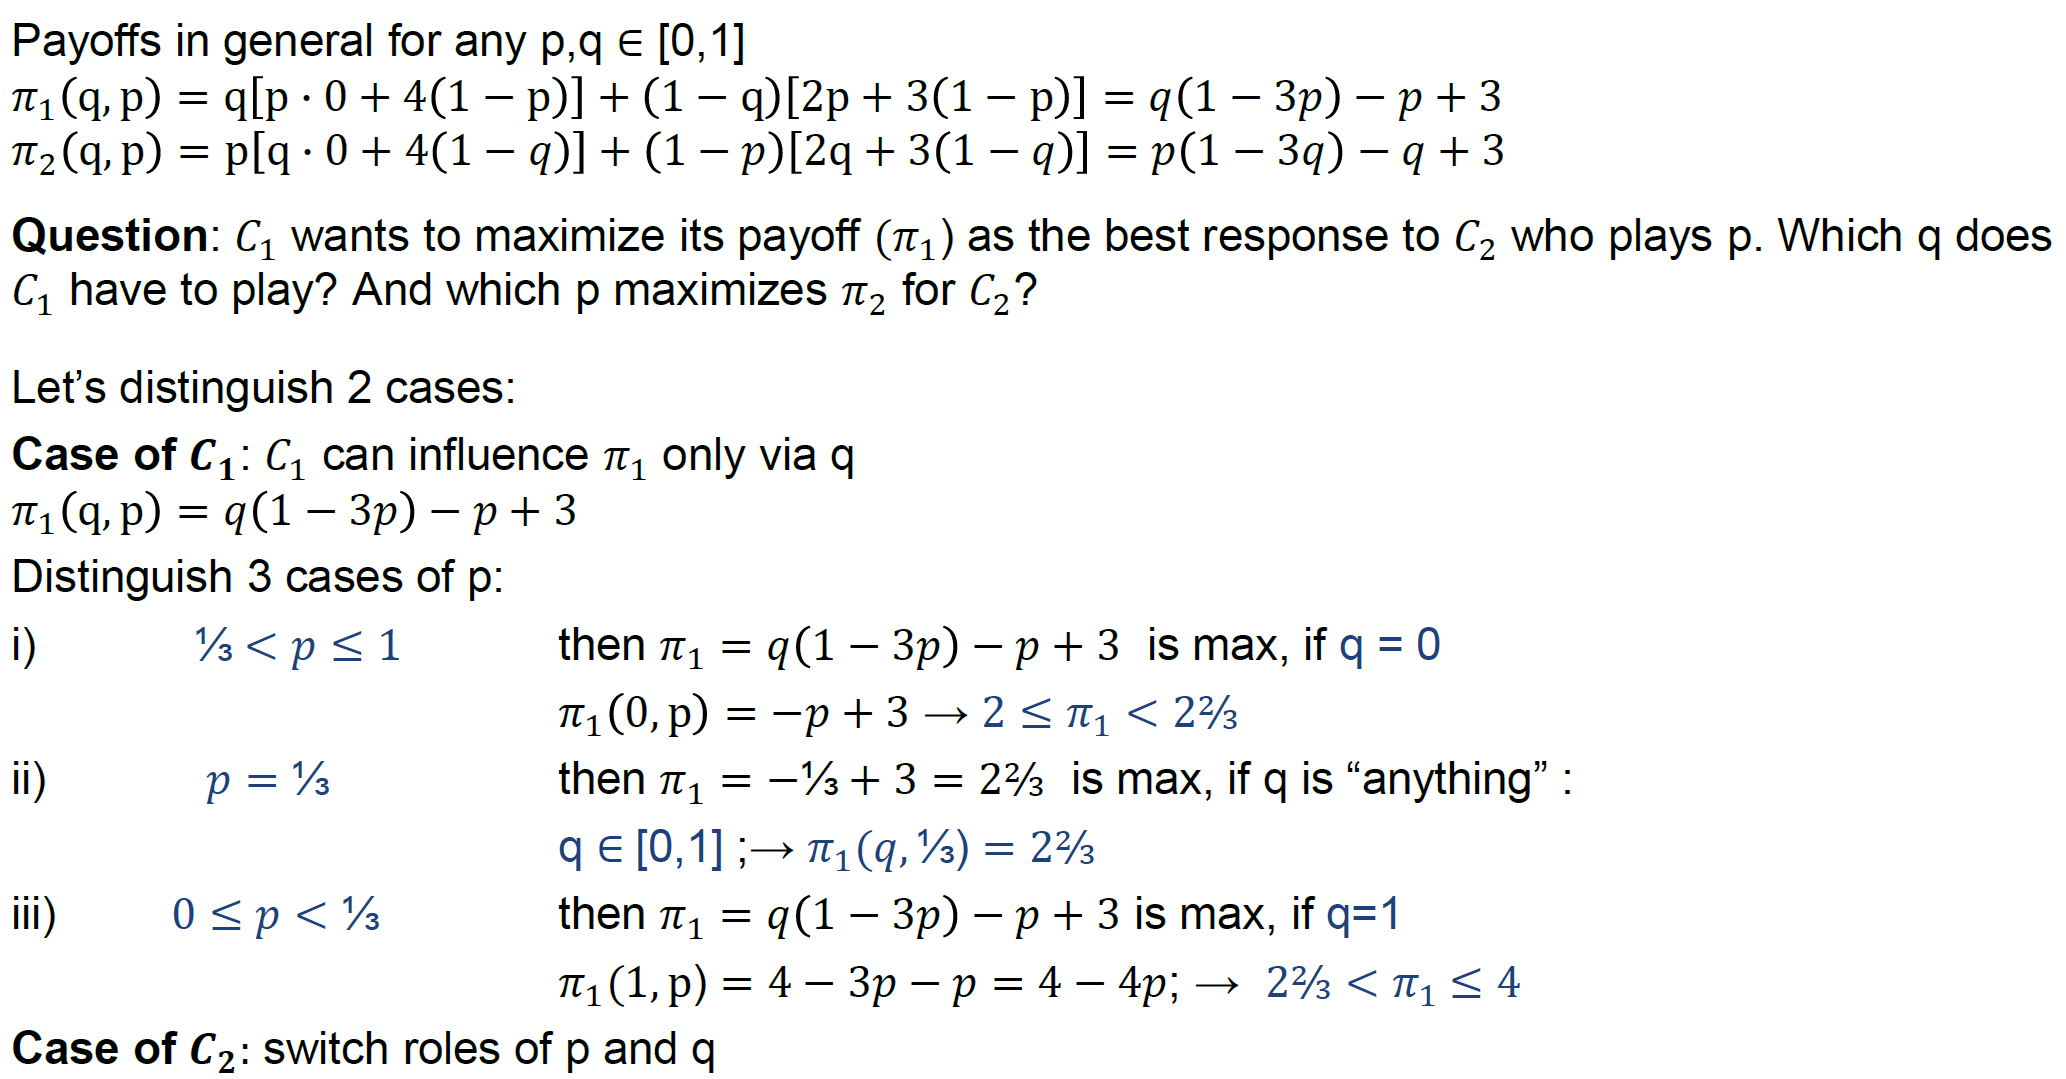
\includegraphics[width=0.7\textwidth]{Pictures/chicken_payoffs.png}
\end{figure}

\begin{figure}[H]
    \centering
    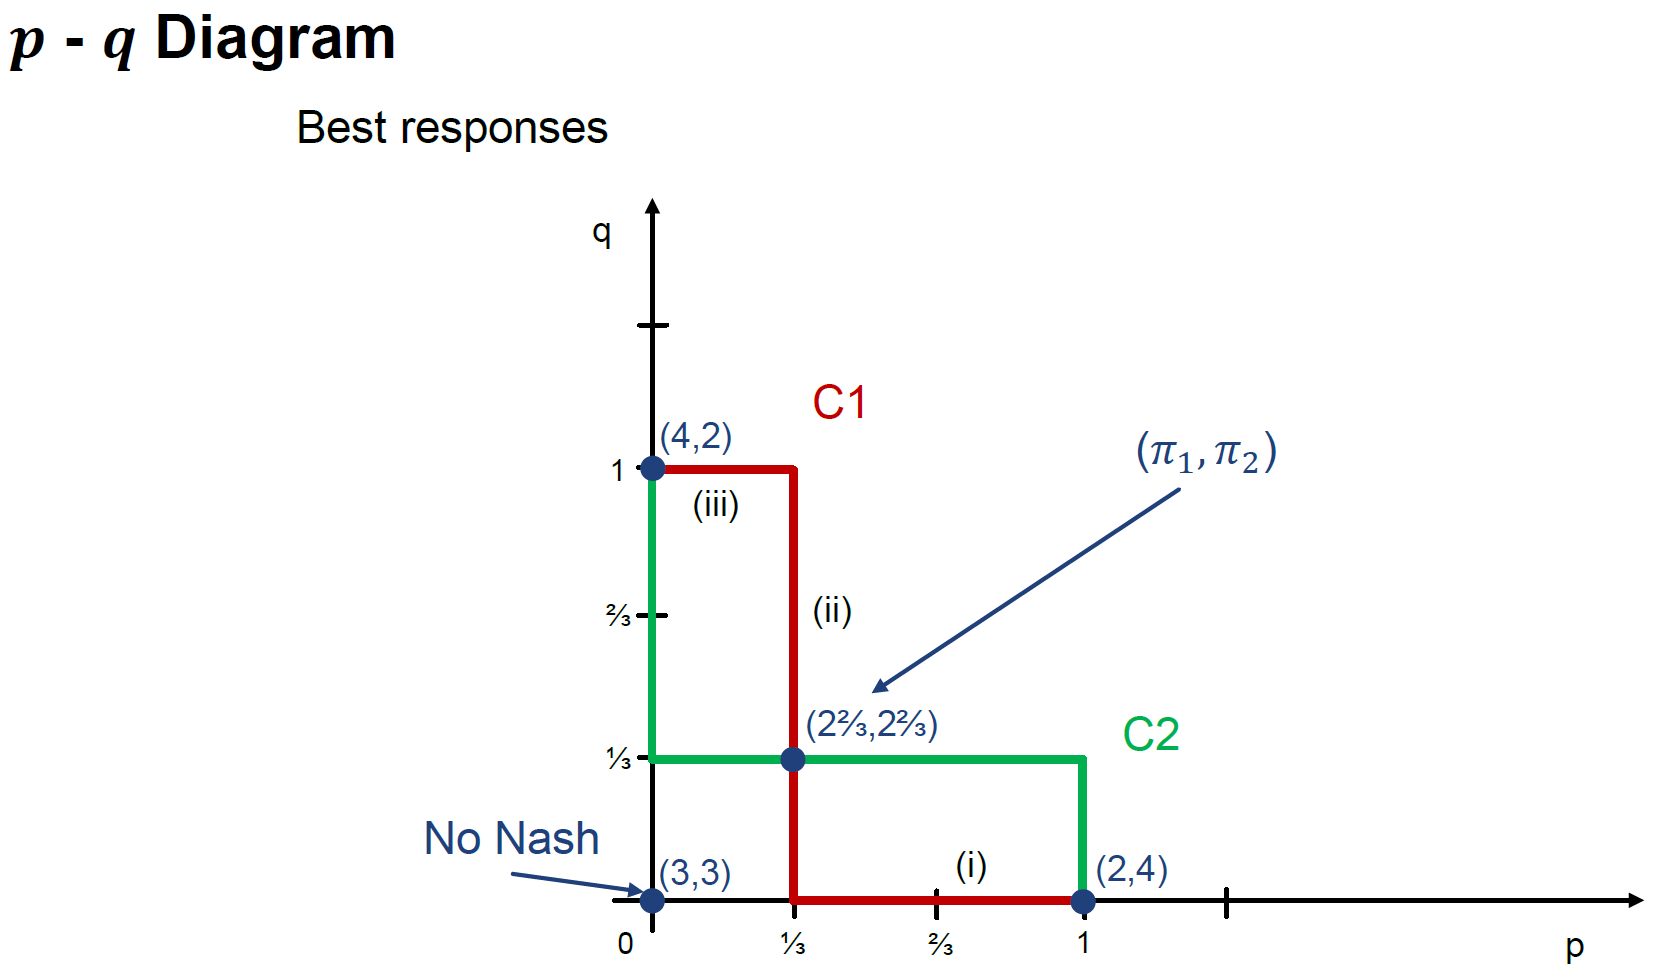
\includegraphics[width=0.5\textwidth]{Pictures/chicken_p_g_diagram.png}
\end{figure}

Comments:
\begin{itemize}
    \item This type of game is often referred to "Chicken" or "Hawk-Dove" game.
        The name is derived from a "sport" in which two drivers race towards each other
        on a narrow road. Each driver has the option to either swerve or to
        continue on a collision course.
    \item In case of multiple equilibria - how to coordinate a particular outcome?
    \item There can be one, many or no Nash equilibria in pure strategy
    \item Existance of Nash Equilibrium: In the normal-form game with a finite
        number of players and each player's strategy set being finite, there
        exists at least one Nash Equilibrium in pure or mixed strategies.
\end{itemize}

\begin{figure}[H]
    \centering
    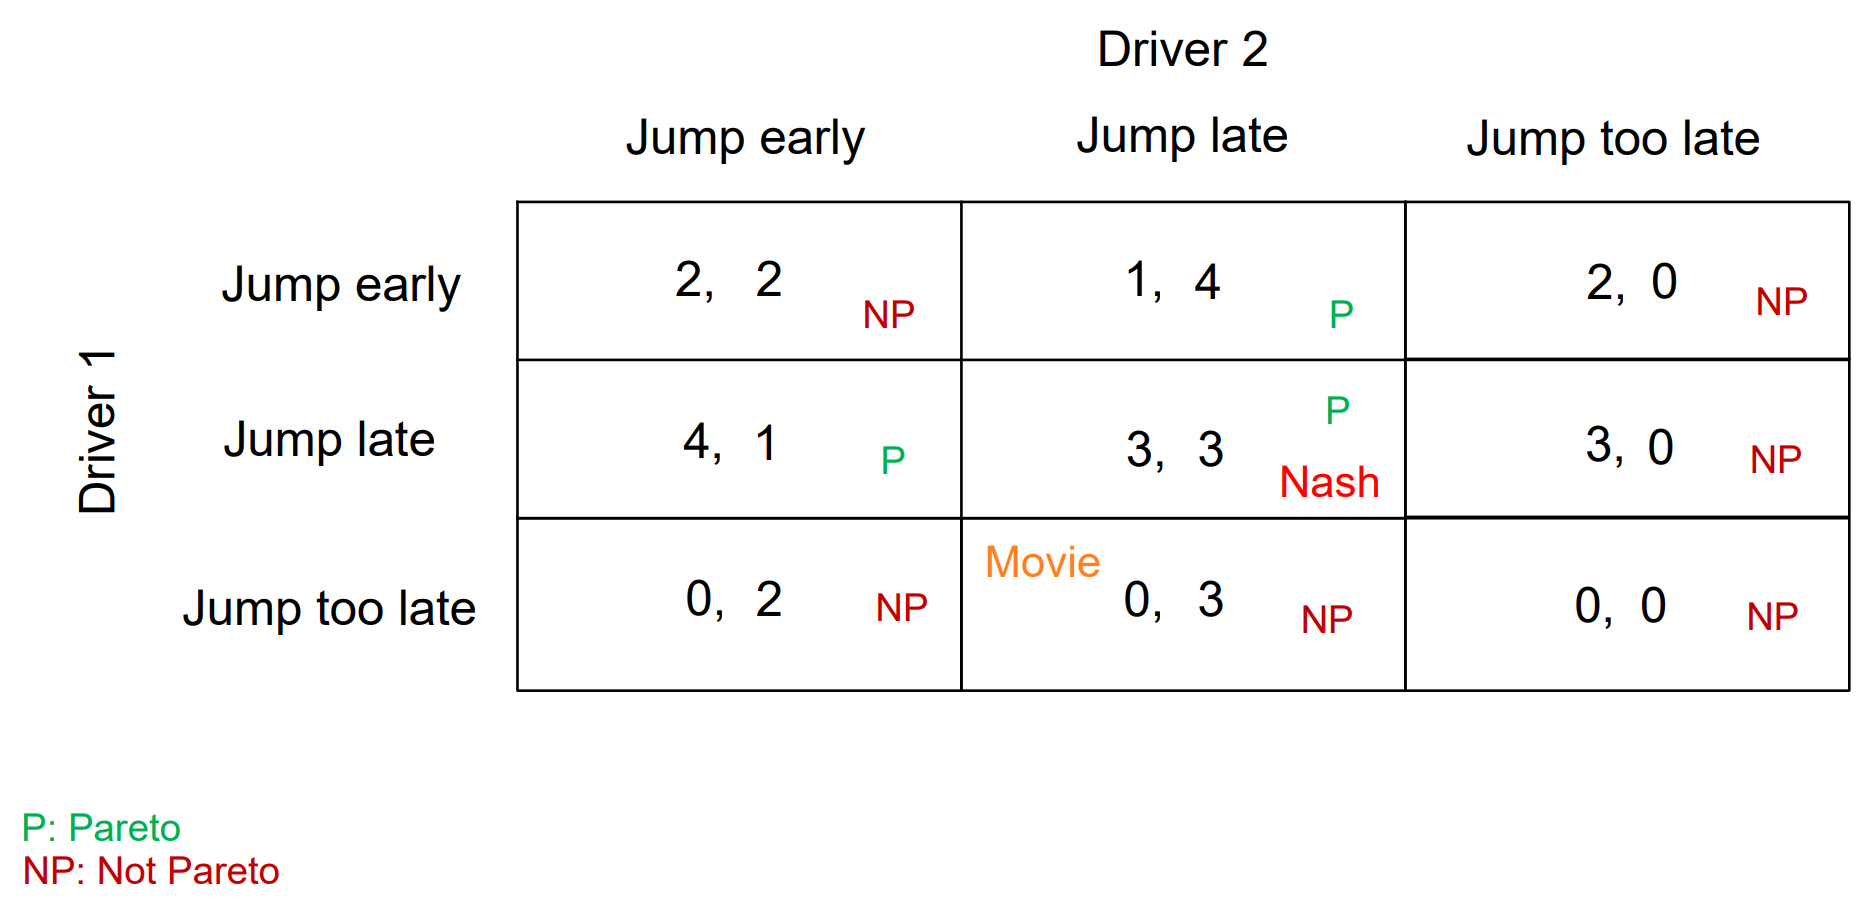
\includegraphics[width=0.6\textwidth]{Pictures/chicken_driver_solution.png}
\end{figure}

\vspace{1\baselineskip}

\underline{Example 15: Stag Hunt}
Situation:
\begin{itemize}
    \item The "Stag Hunt" is a game extracted from Jean Jaques Rousseau's
        "A Discourse on Inequality" which introduces the conflict between
        cooperation and safety.
    \item In this game, each member of a group of hunters has two options:
        he may remain attentive to the pursuit of the stag, or he may catch a hare
    \item If all hunters cooperate to pursue the stag, they catch it and share it
        equally; if any hunter devotes his energy to catching a hare, the stag
        escapes, and the hare belongs to de defecting hunter hunter alone
    \item Each hunter prefers a share of the stag to the hare
\end{itemize}


\begin{figure}[H]
    \centering
    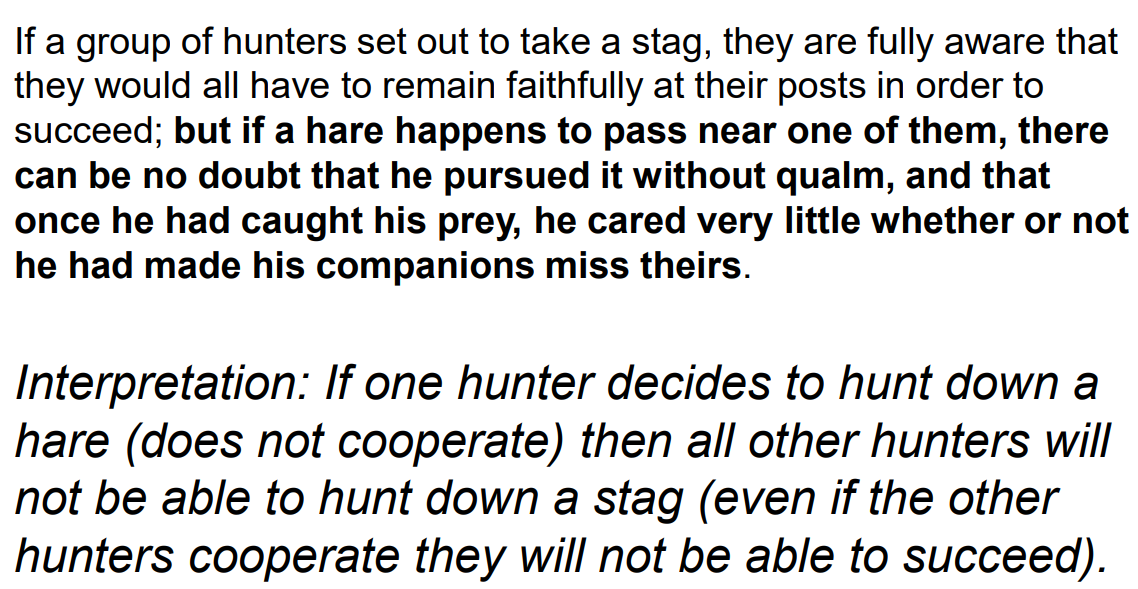
\includegraphics[width=0.5\textwidth]{Pictures/rousseau.png}
\end{figure}

Game:
\begin{enumerate}[(i)]
    \item Players: 2
    \item Actions of players: Stag, Hare
    \item Payoffs are presented in the normal form below
\end{enumerate}

\begin{figure}[H]
    \centering
    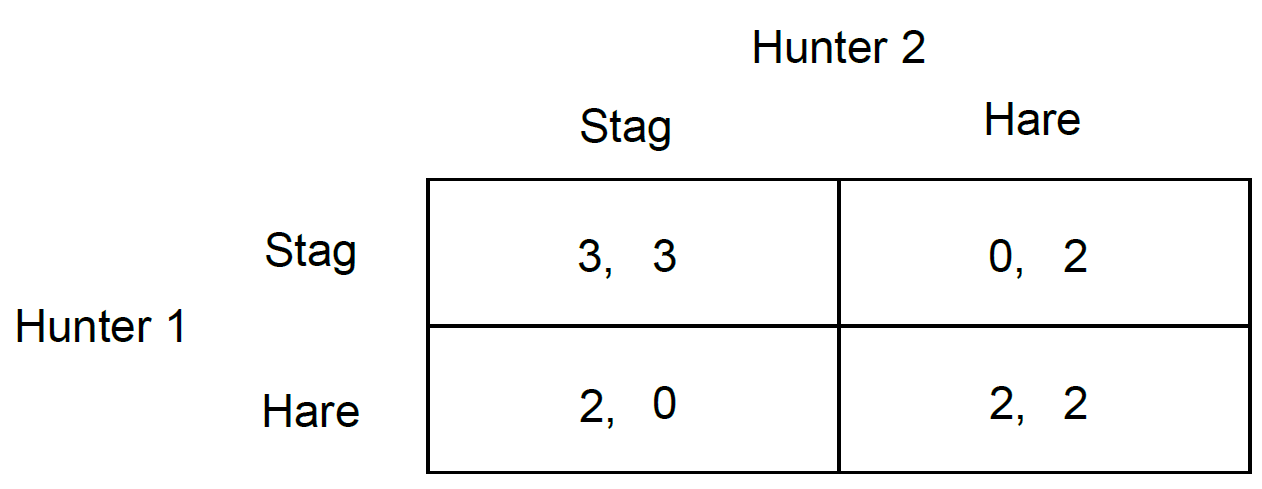
\includegraphics[width=0.5\textwidth]{Pictures/stag_hare_hunter.png}
\end{figure}

\begin{figure}[H]
    \centering
    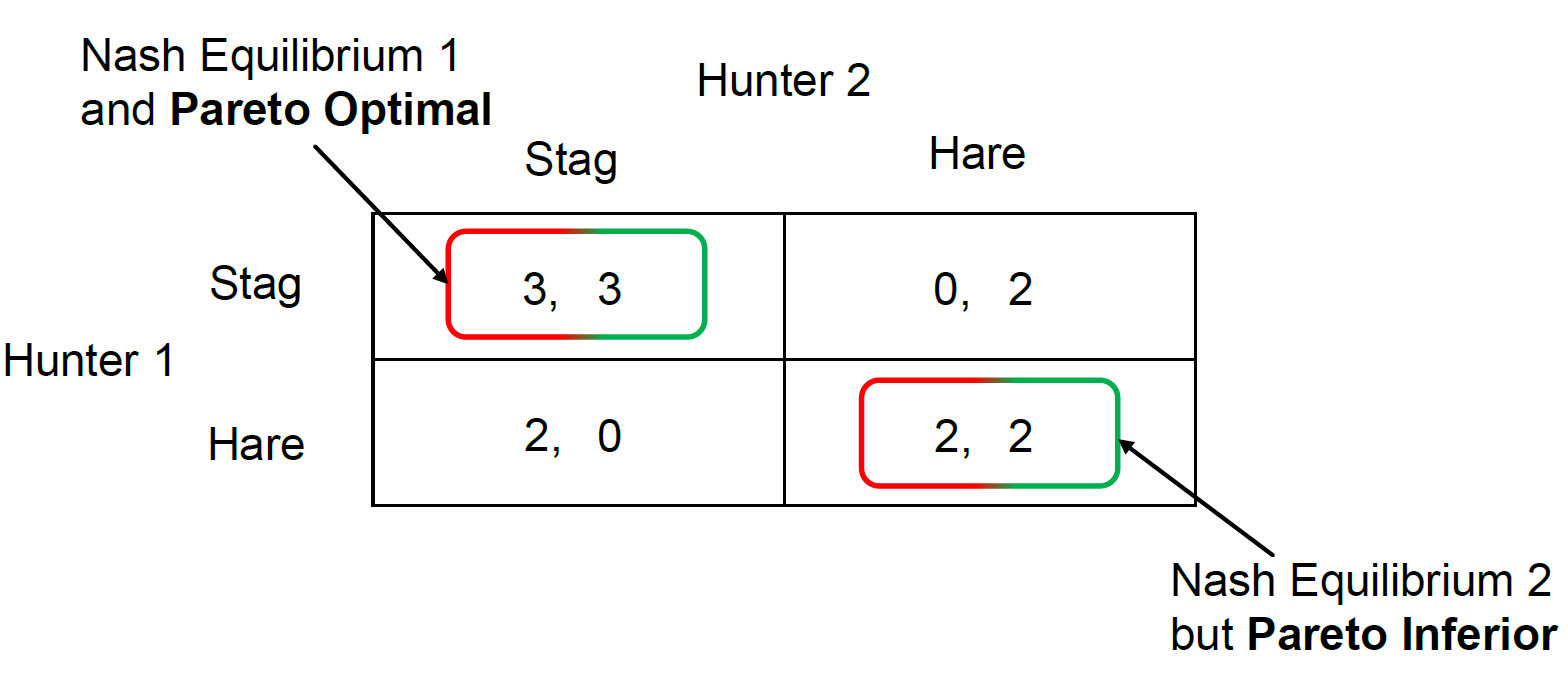
\includegraphics[width=0.5\textwidth]{Pictures/hunter_pure_strategy.png}
    \caption{Pure Strategy}
\end{figure}

\begin{figure}[H]
    \centering
    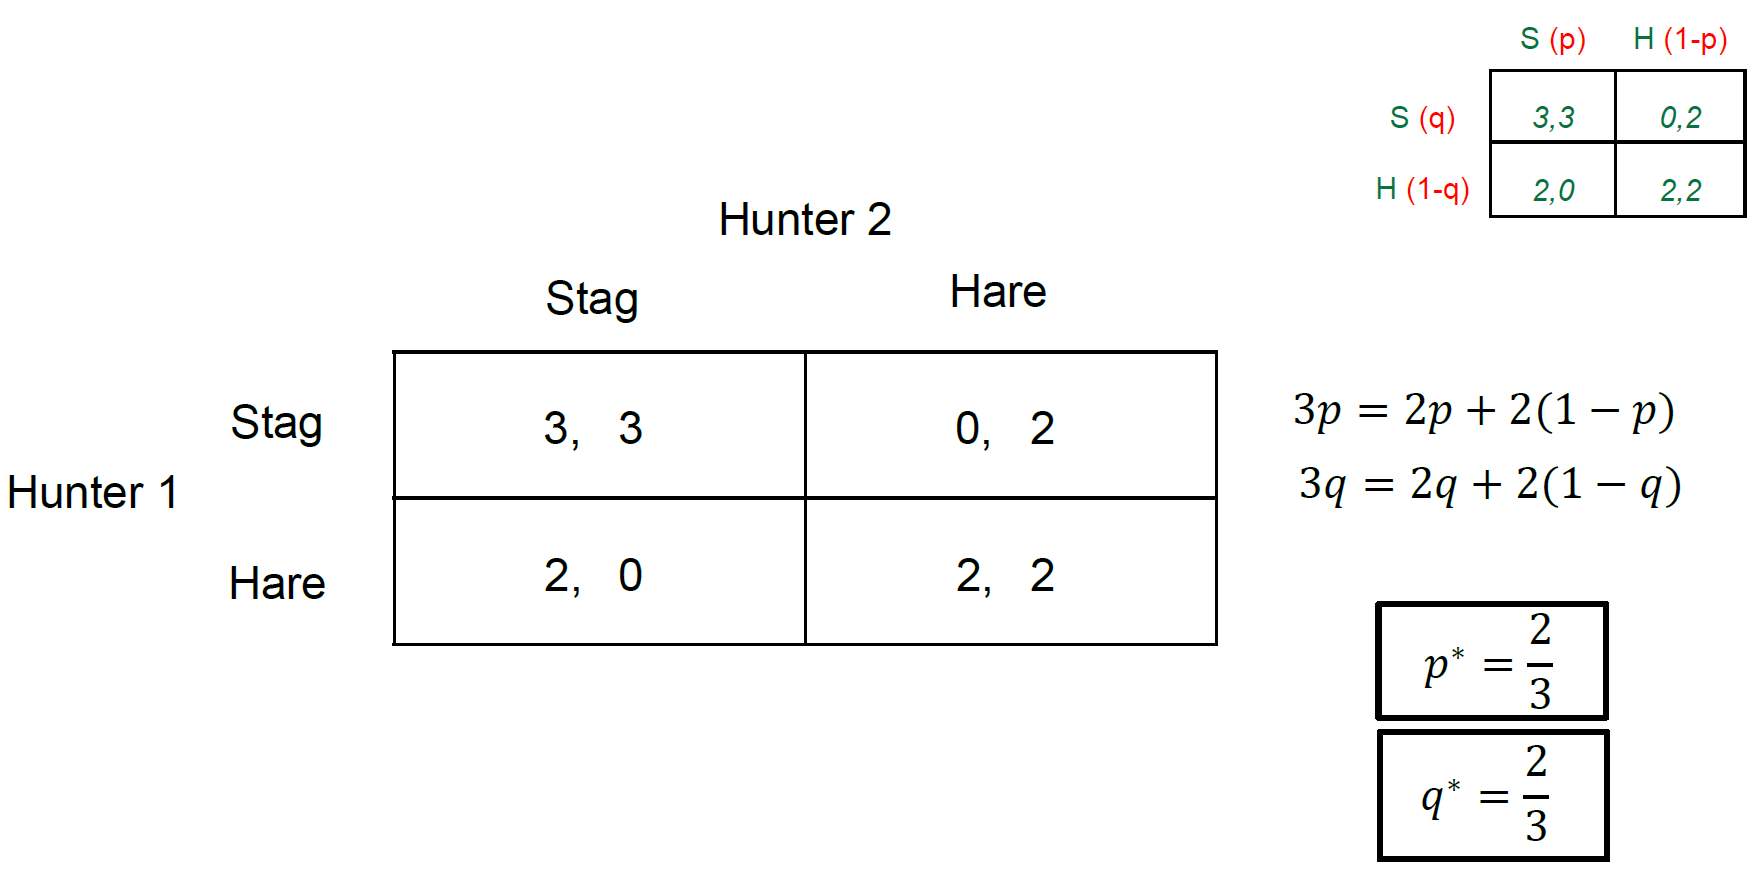
\includegraphics[width=0.5\textwidth]{Pictures/hunter_mixed_strategy.png}
    \caption{Mixed Strategy}
\end{figure}

\begin{figure}[H]
    \centering
    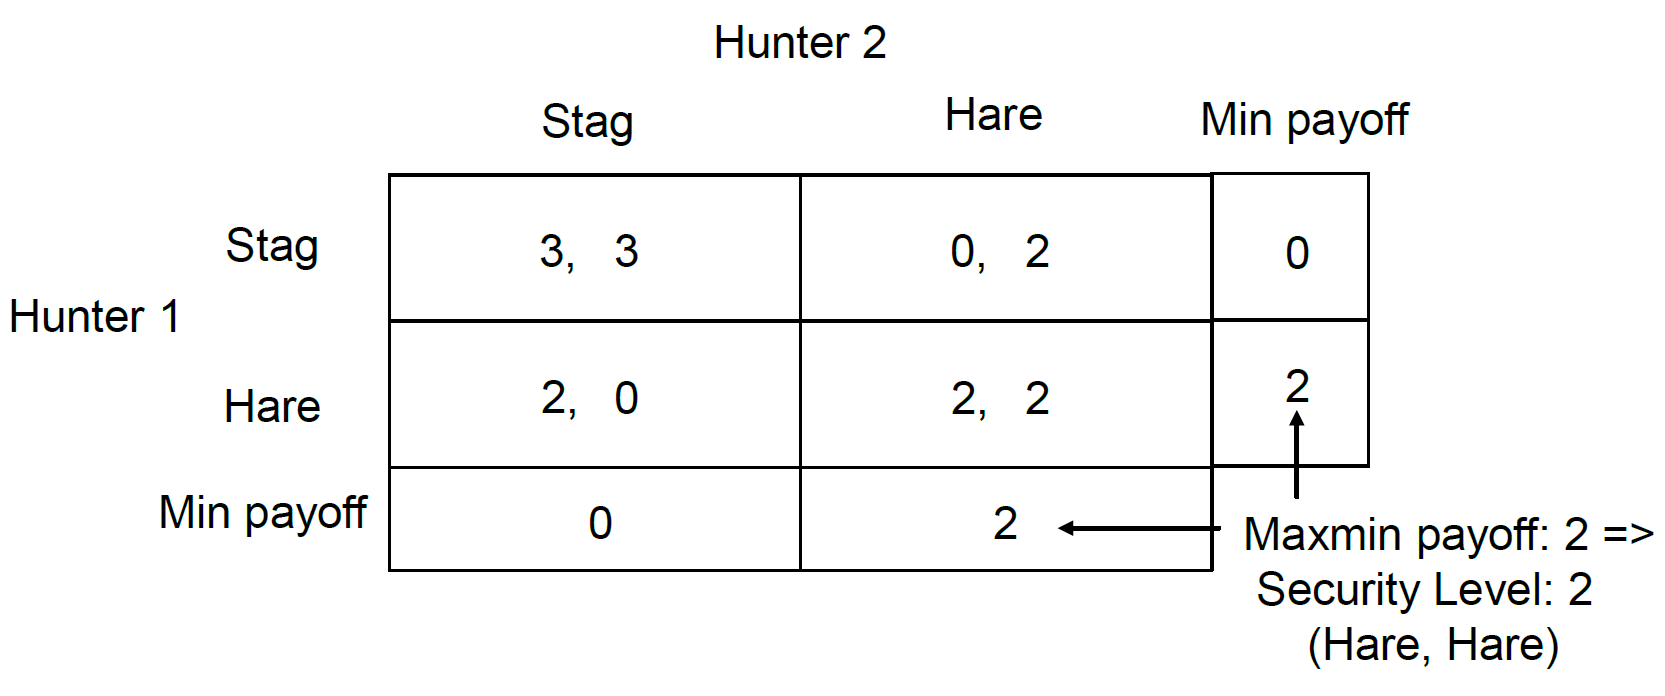
\includegraphics[width=0.5\textwidth]{Pictures/hunter_security_risk_analysis.png}
    \caption{Security Risk analysis}
\end{figure}

\begin{figure}[H]
    \centering
    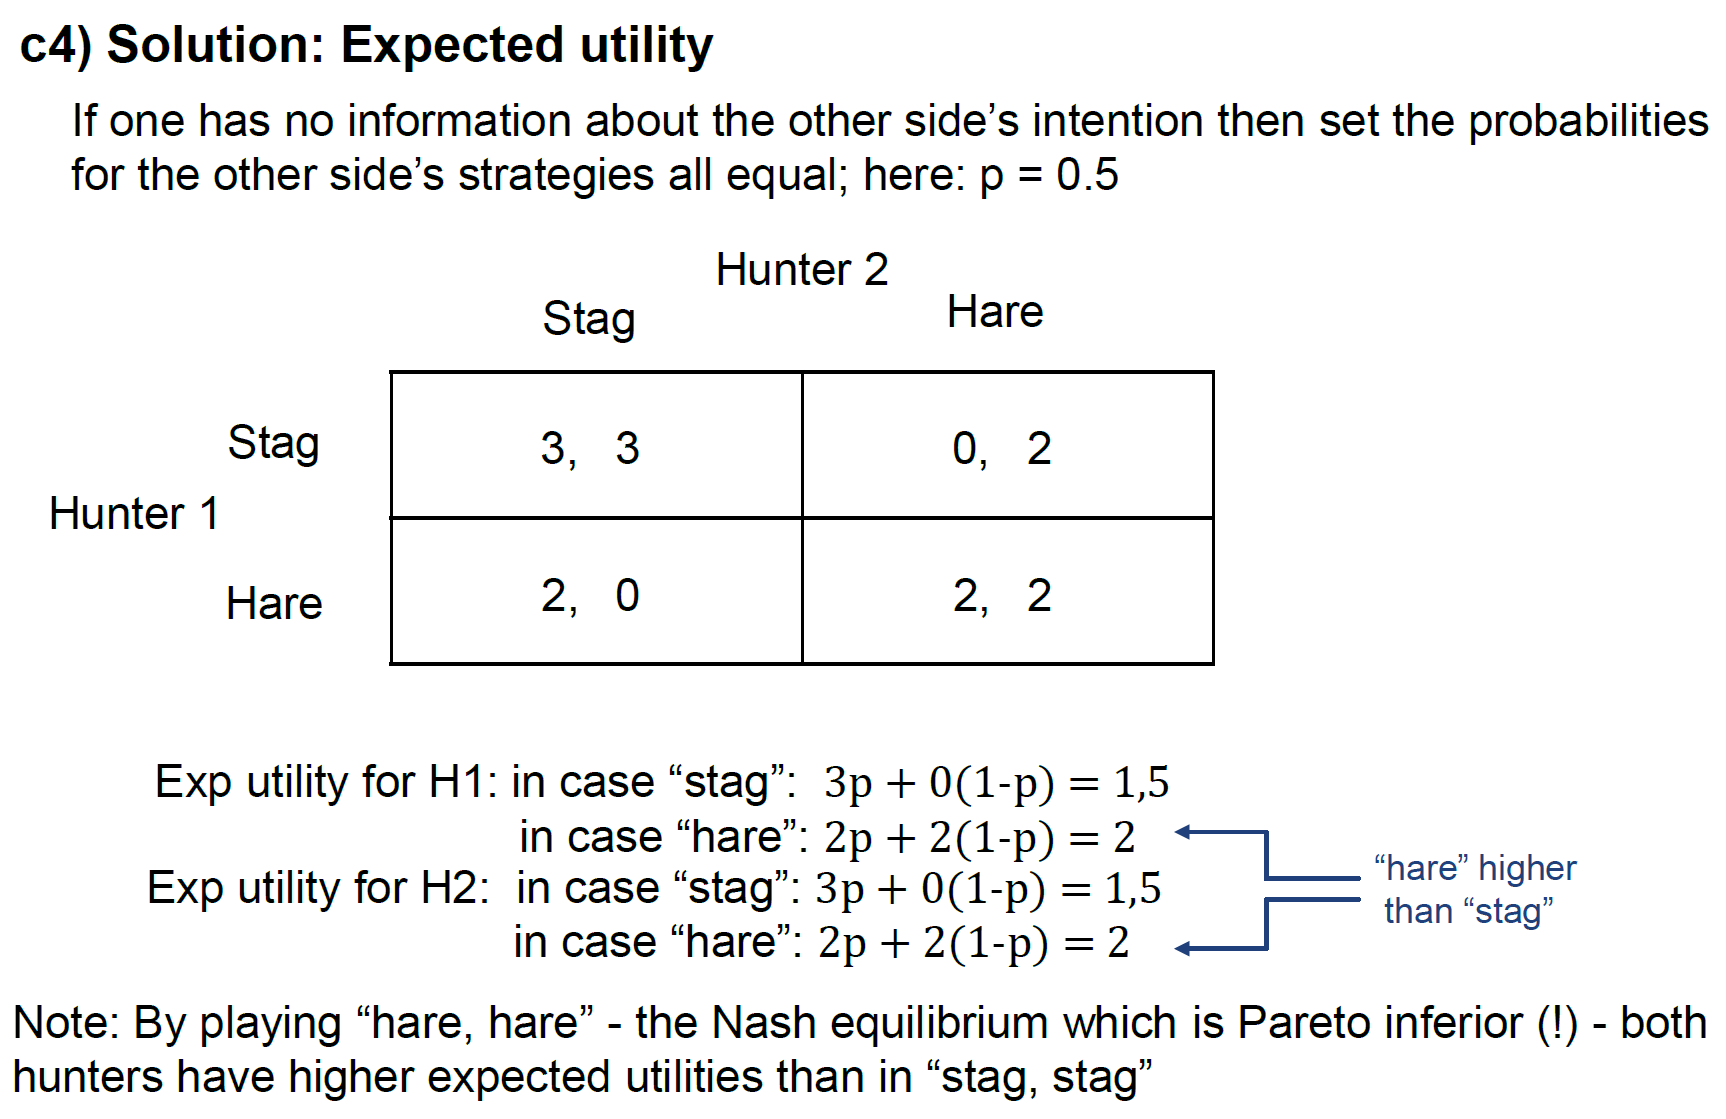
\includegraphics[width=0.5\textwidth]{Pictures/hunter_expected_utility.png}
    \caption{Expected Utility}
\end{figure}

\begin{figure}[H]
    \centering
    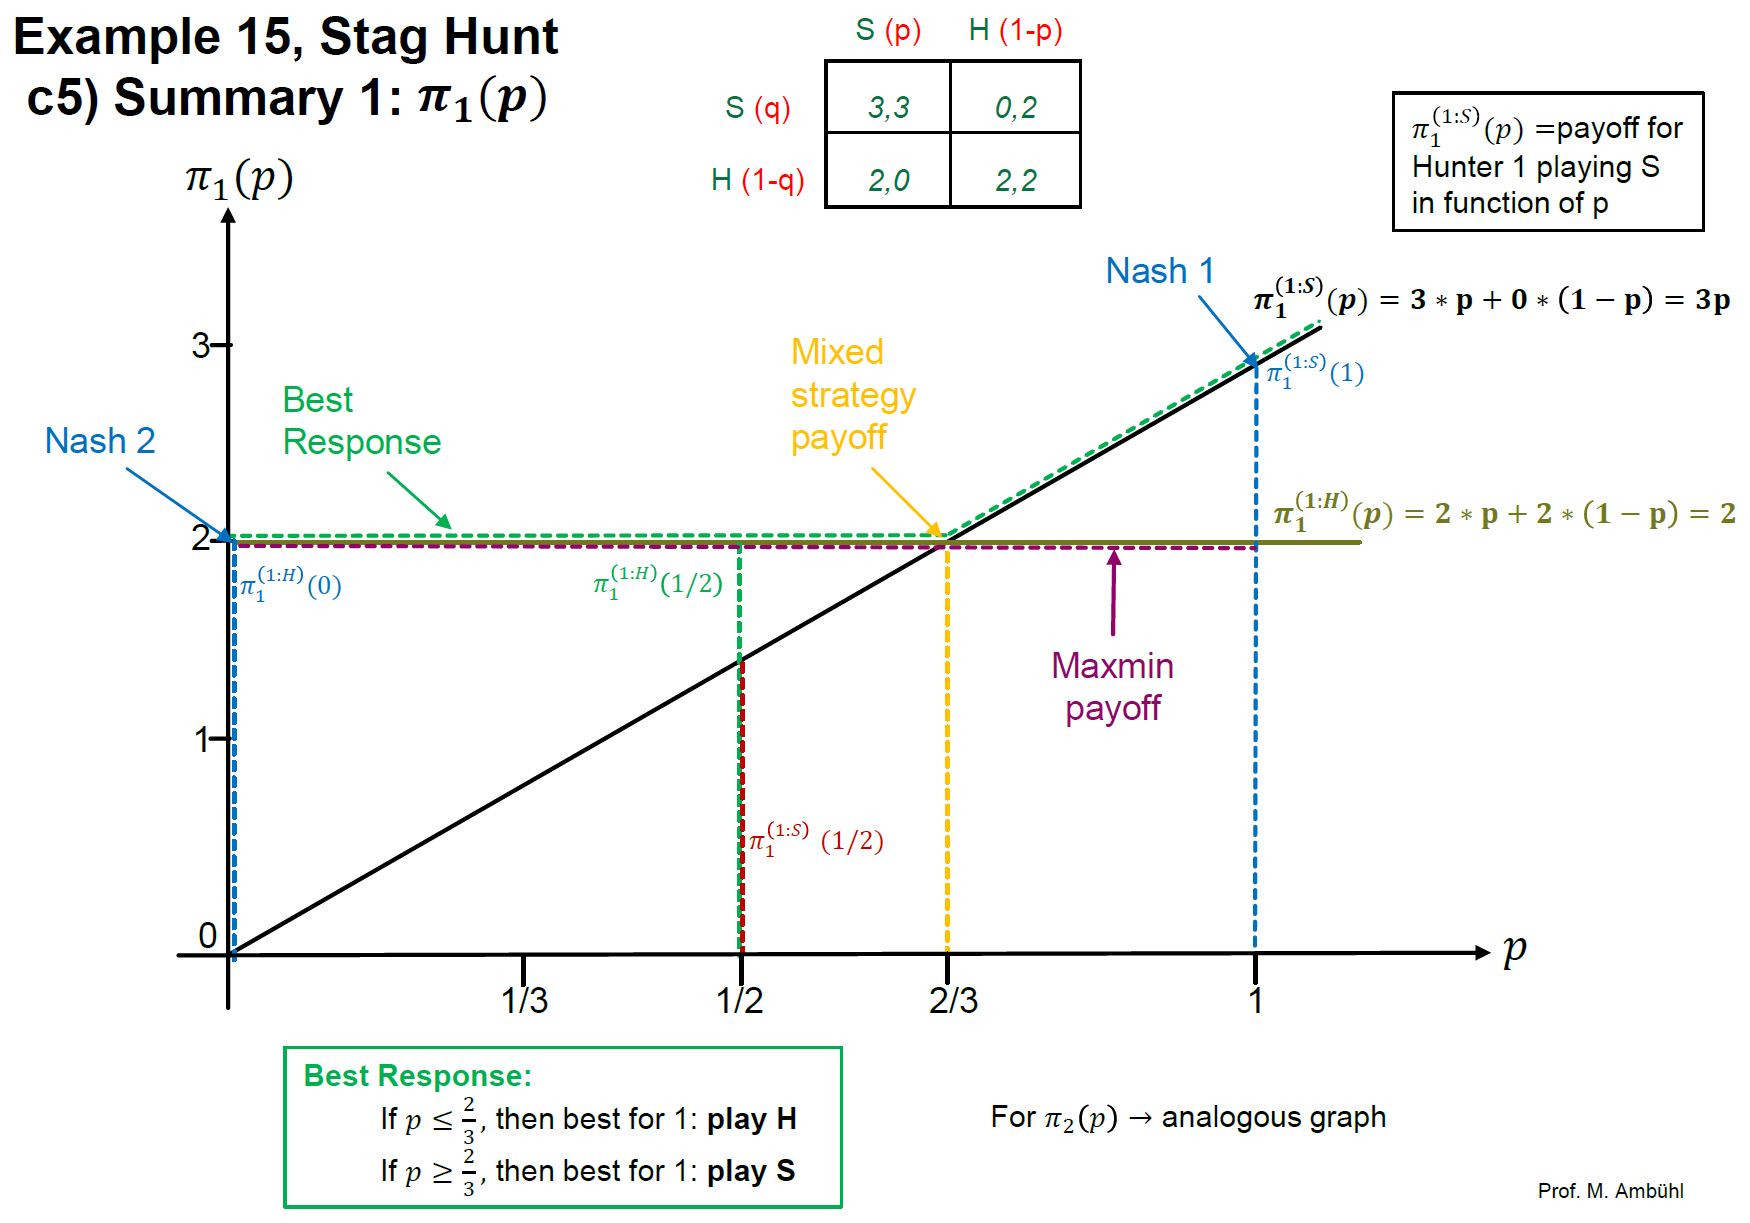
\includegraphics[width=0.5\textwidth]{Pictures/stag_hunt_summary.png}
    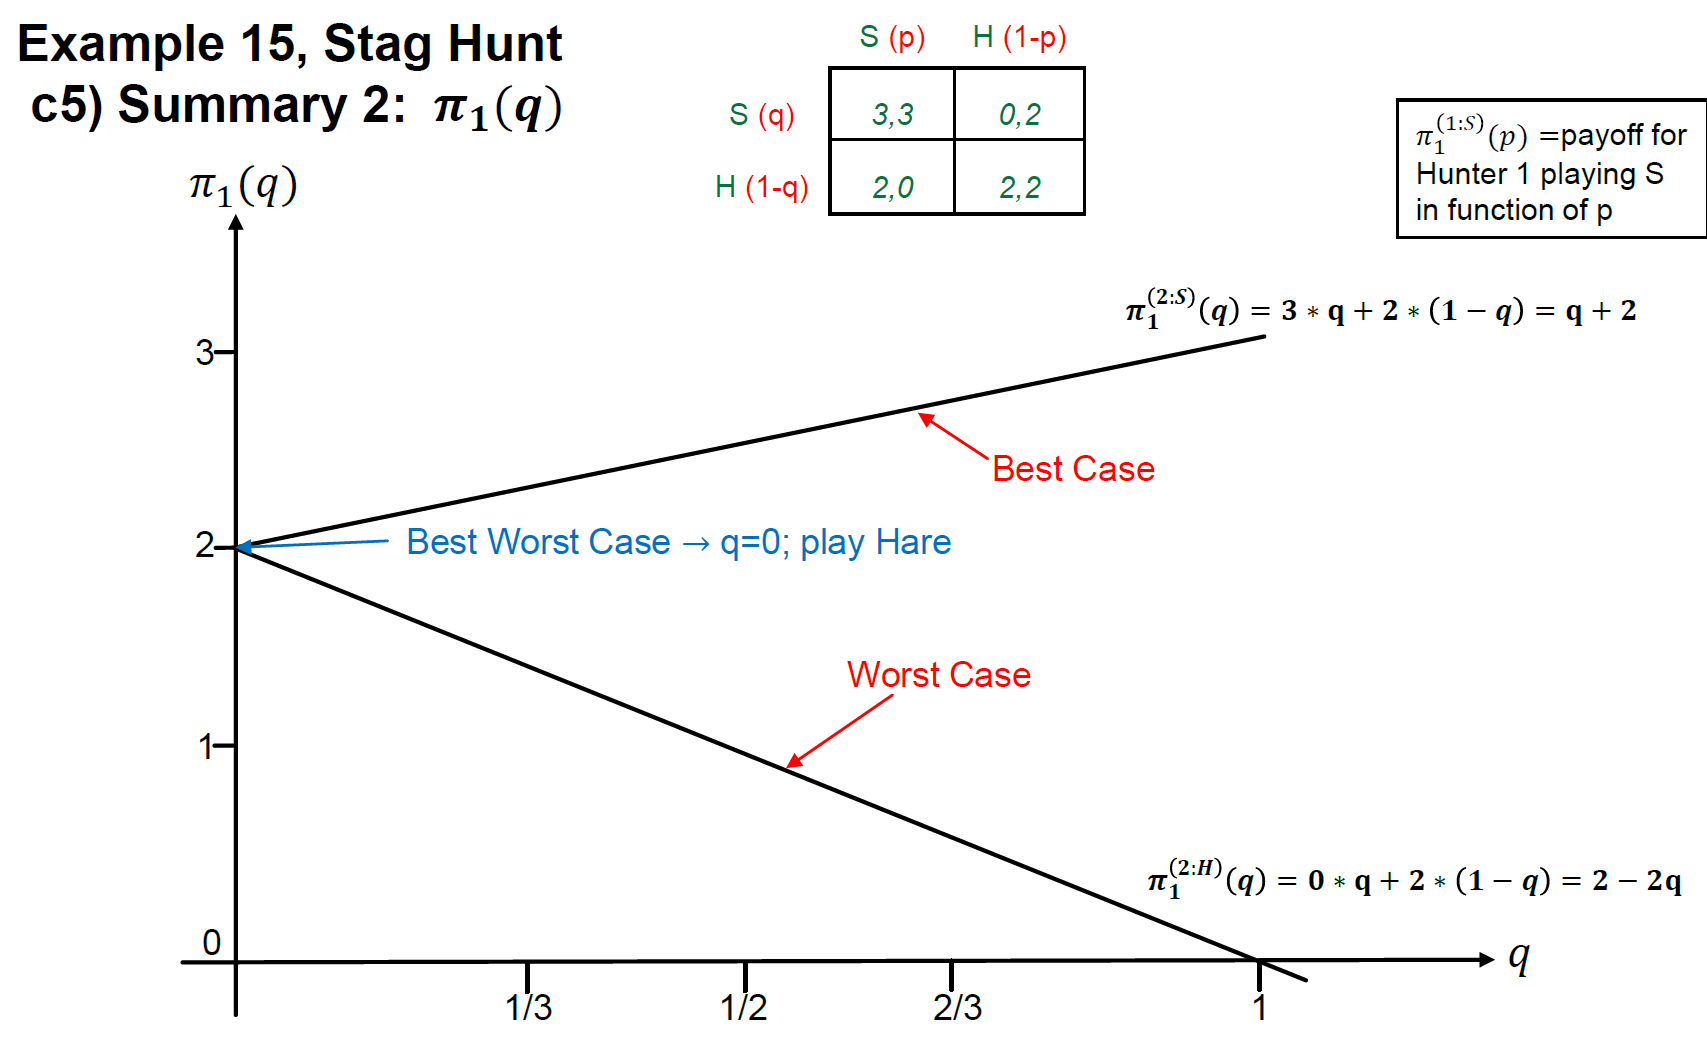
\includegraphics[width=0.5\textwidth]{Pictures/stag_hunt_summary_2.png}
    \caption{Stag Hunt summary}
\end{figure}

\underline{Example 16: 'Arms race' game}
Situation:
\begin{itemize}
    \item Arms race is the process of excessive investment in weapons, military
        technology and the army. Prominent examples:
        \begin{itemize}
            \item Great Britain and Germany competed on having the best navy
                before WW\uproman{1}
            \item Nuclear arms race between the US and the SU
        \end{itemize}
    \item Generally the arms race can be characterized by a country's desire to
        have a military advantage, whenever the counterparty does not arm.
        Staying ahead in military terms allows a country to maintain a
        powerful position.
    \item Whenever all countries are well armed, no one has an advantage,
        but the excessive investment may even hurt the economies.
\end{itemize}

Game:
\begin{enumerate}[(i)]
    \item Players: 3
    \item Actions of players: Arm, Disarm
    \item Payoffs are presented in th enormal form below.
\end{enumerate}

\begin{figure}[H]
    \centering
    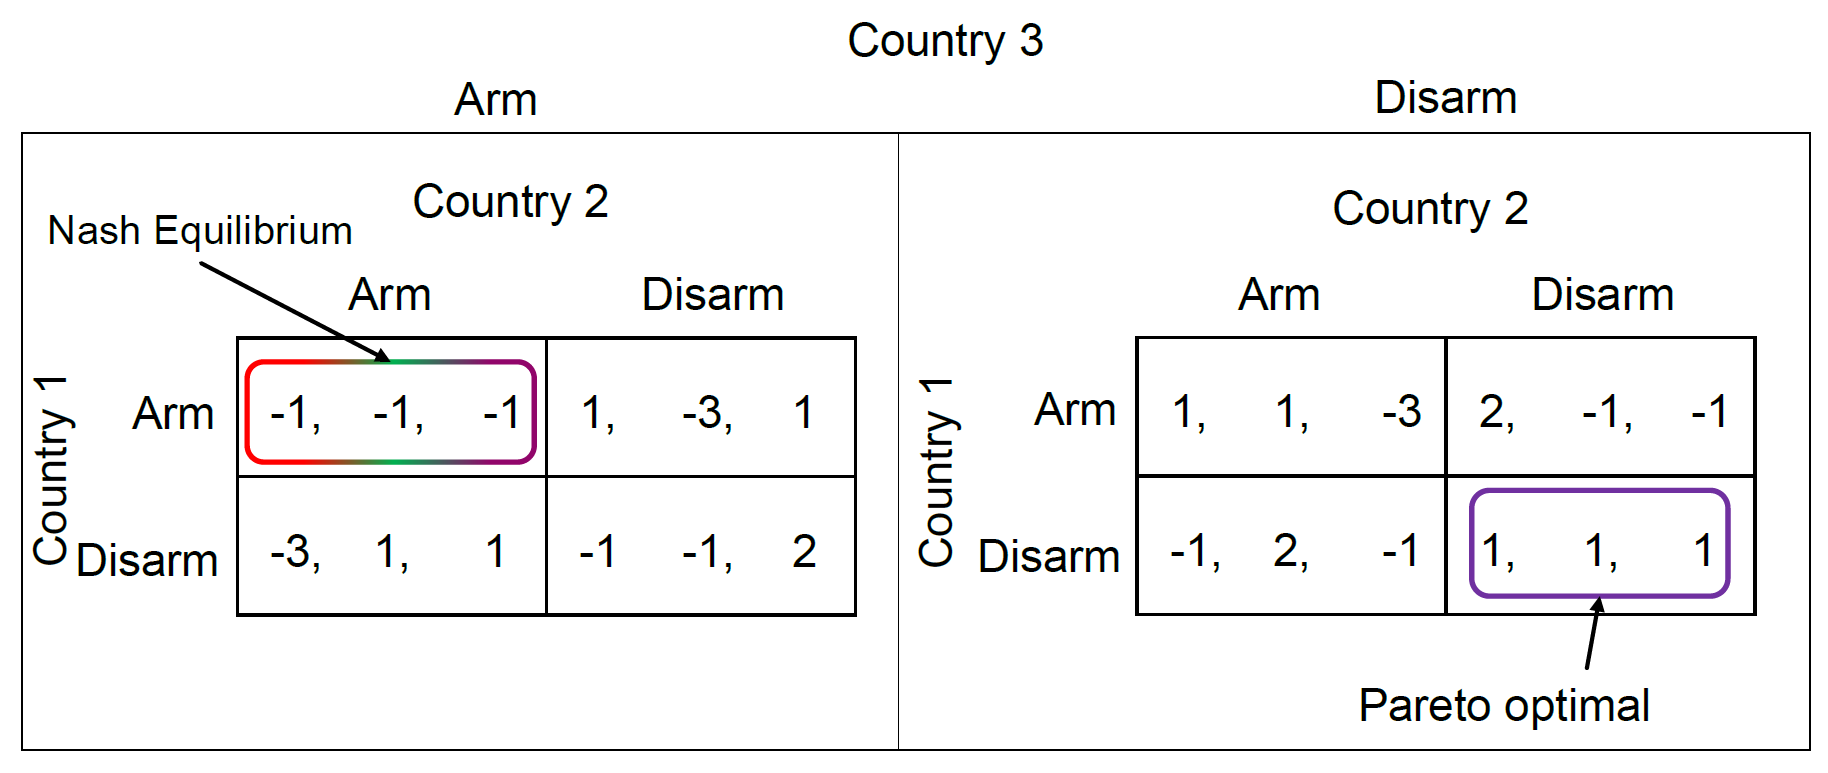
\includegraphics[width=0.6\textwidth]{Pictures/arms_race_nash_equilibrium.png}
\end{figure}

Comments:
\begin{itemize}
    \item Example $16$ illustrates the "non-cooperative simultaneous move"
        game in the normal form in case of $3$ players.
    \item Arms race is another example of the Prisoners' Dilemma: Every country
        is better off when no one increases their military capabilities, but this
        cooperative outcome is not sustainable as a Nash Equilibrium.
\end{itemize}

\vspace{1\baselineskip}

\underline{Example: Turkey Greece refugee question}

\begin{figure}[H]
    \centering
    \includegraphics[width=0.8\textwidth]{Pictures/turkey_greece_refugees.png}

    \vspace{1\baselineskip}

    \includegraphics[width=0.8\textwidth]{Pictures/turkey_greece_refugees_2.png}
\end{figure}

\underline{Example}

\vspace{1\baselineskip}

17 Camels should be distributed to $3$ children according to the following
distribution:
\begin{itemize}
    \item $\frac{1}{2}$ goes to the oldest son
    \item $\frac{1}{3}$ goes to the middle son
    \item $\frac{1}{9}$ goes to the youngest son
\end{itemize}

\begin{figure}[h]
    \centering
    \includegraphics[width=0.9\textwidth]{Pictures/Camel_solutions.png}
    \caption{Solution to the Camel problem}
\end{figure}


\paragraph{Dynamic Games}

\begin{itemize}
    \item Contrary to a static game, in a dynamic game players take action
        over time.
    \item A static game can be seen as one 'one-shot' game, whereas in a dynamic
        game a player can move more than once.
    \item We will consider dynamic games of perfect information, i.e. games in
        which each player, when taking an action, is perfectly informed of all
        the events that have previously occured.
\end{itemize}

\subparagraph{Sequential move games}

\begin{itemize}
    \item In sequential move games players have some knowledge about earlier
        actions of the game, i.e. decisionmaking happens sequentially - one
        player takes his action before the other does.
\end{itemize}

\vspace{1\baselineskip}

\underline{Example 17: 'Nuclear deterrence' game}

\begin{enumerate}[a)]
    \item Situation in words:
        \begin{itemize}
            \item During the Cold War, the US and SU had big nuclear
                arsenals and neither side could 'disarm' the other side with
                just the first nuclear strike - each side secured second strike
                capabilities - both could have responded to any nuclear strike
                with a devastating retaliatory strike (e.g. from submarines)
            \item Knowing this, consider now the situation where one country
                decides first whether to launch an attack or to delay it. In case
                it delays an attack, the second country can make its own decision
                whether to attack or not.
            \item When both countries delay an attack, the status quo is preserved
            \item Whenever there is an attack, both aggressor and defender suffer
                from the nuclear war, however there is a slight first-mover advantage
                in comparison to the defender.
        \end{itemize}
    \item Game
        \begin{enumerate}[(i)]
            \item Players: 2
            \item Strategies of players: Attack, Delay
            \item Sequence of moves is shown in the extensive form game
                (e.g. in the game tree)
            \item Payoffs are given in the terminal nodes (i.e. places where the game
                tree ends).
        \end{enumerate}
        \begin{figure}[H]
            \centering
            \includegraphics[width=0.5\textwidth]{Pictures/nuclear_example_1.png}
        \end{figure}
    \item Solution
        \begin{enumerate}[c1)]
            \item Some definitions:
                \begin{enumerate}[(1)]
                    \item A subgame is a part (sub-tree) of a game that satisfies
                        the following conditions:

                        a) It begins at a decision node (for any player)

                        b) The player knows all the decisions that have been
                            made up until that time

                        c) The sub-tree contains all the decision nodes that
                            follow the initial node (and no other)
                            
                        Example: There are two subgames in Example 17
                    \item A strategy is a rule for choosing an action at every point
                        that a decision might have to be taken by the player. A strategy
                        is a complete plan of actions.
                \end{enumerate}
            \item Backwards Induction and Subgame Perfect Nash Equilibrium
                \begin{itemize}
                    \item The most common way of solving dynamic games is through
                        backwards induction. In this procedure, the last player
                        to act at each node chooses the action that maximizes
                        his utility (i.e. the Nash Equilibrium)

                        The second to last player then chooses his action optimally,
                        knowing that the last player chooses optimal actions at each
                        node. This process continues until each player has chosen
                        optimally under the assumption that all future players
                        make optimal choices.
                    \item Applying backwards induction always results in a pure
                        strategy Nash Equilibrium (i.e. there is always at least
                        one Nash Equilibrium in pure strategy)
                    \item The resulting equilibrium is called a \textit{Subgame
                        Perfect Nash Equilibrium} as it induces a Nash Equilibrium
                        in every subgame of the whole game.
                    \item The concept of subgame perfection was formulated by Reinhard
                        Selten.
                \end{itemize}
            \item Solution to example 17:
                
                In Subgame Perfect Nash Equilibrium both countries decide to delay.
        \end{enumerate}
    \item Comments:
        \begin{itemize}
            \item This model assumes the order of moves: First is Country $1$
                and second is country $2$. (In reality, however, both countries
                can pretend to be the first to move and both countries can be
                unsure whether delaying a move will transition to the status quo
                or give the other side the opportunity to launch its own strike.)
                
                $\rightarrow$ More elaborate games (e.g. game with imperfect
                information) may be better suited for analysis.
            \item Subgame Perfect Nash Equilibrium is a more suitable solution
                concept for dynamic games than just Nash Equilibrium - it rules
                out some 'unrealistic' Nash Equilibrium predictions (see Exercise
                Session)
        \end{itemize}
\end{enumerate}

\vspace{1\baselineskip}

\underline{Example 18: 'Political crisis' game}

\begin{enumerate}[a)]
    \item Situation:
        \begin{itemize}
            \item In a country there is a conflict between the government and
                the opposition.
            \item The Government has now the choice between proposing a broad
                package of reforms or escalating the conflict by calling in the
                army
            \item In case the reforms are proposed, the opposition can decide
                whether to accept them or to continue the protests.
            \item In case the military option is chosen, the opposition
                decision is reduced to either giving-in or resisting.
        \end{itemize}
    \item Game:
        \begin{enumerate}[(i)]
            \item Players: 2
            \item Action of players:
                \begin{itemize}
                    \item Government: Reform, Escalate
                    \item Opposition:
                        \begin{itemize}
                            \item In the case of Reform is chosen: Accept, Reject
                            \item In the case of Escalate is chosen: Give-in, Resist
                        \end{itemize}
                \end{itemize}
            \item Sequence of moves is shown in the extensive form game (e.g. in the game tree)
            \item Payoffs are given in the terminal nodes.
            \begin{figure}[H]
                \centering
                \includegraphics[width=0.7\textwidth]{Pictures/political_crisis_example.png}
            \end{figure}
        \end{enumerate}
    \item Solution:
    
        Subgame Perfect Nash Equilibrium:
        \begin{itemize}
            \item Government: Plays Reform strategy (Because, if they play
                Escalate, the opposition will play Resist)
            \item Opposition: Plays Accept, if Reform is observed and plays
                Resist, if Escalation is observed from the government side
        \end{itemize}
    \item Comment
        \begin{itemize}
            \item Example 18 illustrates the concept of a strategy in a dynamic
                game. A strategy is a complete list of actions. Thus it prescribes
                an optimal action even in the decision nodes, which are not reached
                by the equilibrium play of the game.
        \end{itemize}
\end{enumerate}

\subparagraph{Repeated simultaneous move games}

A repeated game consists of some number of iterations of a simultaneous move game
(i.e. the stage game). A repeated game can be either finite (i.e. with a finite
number of repetitions) or infinite (e.g. without a time horizon).

\vspace{1\baselineskip}

\underline{Example 19: 'Infinite interactions' game}

\begin{enumerate}[a)]
    \item Situation:
        \begin{itemize}
            \item Recall: In Example 13 the Nash Equilibrium was when both
                sellers chose low prices. However, if both choose high prices,
                both will win. (See Example 13)
            \item In reality, competing sellers meet each other every day, i.e.
                they play the game from Example 13 many times in a row, possibly
                an infinite amount of times.
            \item Can the Pareto efficient outcome be achieved, if the game
                is repeated infinitely many times?
        \end{itemize}
    \item Game:
        \begin{enumerate}[(i)]
            \item Players: 2
            \item Actions of players in each stage of the game: high, low
            \item Discounted Payoffs:
                \begin{itemize}
                    \item Each seller discounts his future payoff - discount factor $0 < \delta < 1$
                    \item Total payoff to player $i$ is $\sum_{t=0}^\infty \delta^t \cdot r_i(t)$
                        where $r_i(t)$ is a payoff received in stage $t$.
                \end{itemize}
        \end{enumerate}
    \item Solution
        \begin{enumerate}[c1)]
            \item Concept:
                \begin{itemize}
                    \item In every stage of the game players can choose an
                        action: High or Low price
                    \item There are several tactics that players should play
                        depending on the history of the game. One of them is the
                        so called "Grim Trigger" strategy. This strategy is
                        specified as follows:
                        \begin{itemize}
                            \item start by setting High price (i.e. cooperate with the other player)
                            \item continue with High price until either player sets Low price
                                (i.e. until you or him defect)
                            \item then set Low price forever.
                        \end{itemize}
                \end{itemize}
            \item Solution to Example 19:
                \begin{itemize}
                    \item Suppose Seller $2$ sticks to the Grim Trigger strategy,
                        then if Seller $1$ sets the High Price, it will establish
                        a cooperation in the long run. This generates flow of
                        utility $\sum_{t=0}^\infty \delta^t \cdot 300 = \frac{300}{1-\delta}$
                    \item Suppose now Seller $1$ decides to deviate in the first stage and sets the
                        low price (which brings him an immediate return of $500$). According to
                        the Grim Trigger strategy, Seller $2$ will set the low price in the next
                        round. This generates flow of utility:
                        $500 + \sum_{t=1}^\infty \delta^t \cdot 250 = 500 + \frac{250 \cdot \delta}{1 - \delta}$
                    \item Neither of the sellers will find it profitable to deviate if:
                        $\frac{300}{1 - \delta} > 500 + \frac{250 \cdot \delta}{1 - \delta}$,
                        or $\delta > \frac{200}{250} =  0.8$
                \end{itemize}
        \end{enumerate}
\end{enumerate}

\vspace{1\baselineskip}

\underline{Example 20: Repeated Prisoners' Dilemma}

There are other strategies which achieve cooperation; one of the most successful
strategies in experiments was "Tit-fot-Tat".

\begin{itemize}
    \item In negotiation you often have multiple phases/rounds.
    \item "Tit for Tat" strategy ("As you to unto me, so I do unto you") is
        a famous strategy (in game theory) for repeated games, developed by
        Anatol Rapoport for an experiment by Robert Axelrod:
        \begin{itemize}
            \item begin by playing cooperatively
            \item then do whatever the other player did in the last stage
        \end{itemize}
    \item "Tit for Tat" is a remarkably good and robust strategy for playing
        iterated Prisoner's Dilemma.
    \item Such s strategy should follow these principles:
        \begin{itemize}
            \item Nice: Start by cooperating, and never be the first to defect
            \item Retaliation: Reliably punish defection by the opponent
            \item Forgiving: If you punish defection, be willing to try to
                cooperate again.
            \item Clear: The pattern should be consistent and easy to predict
                (by the opponent)
        \end{itemize}
    \item Is is a cooperation strategy of "friendly reciprocity"
\end{itemize}

\subsubsection{Cooperative Games}

\paragraph{Introduction}

Concept: Players talk to each other to decide on a reasonable or fair outcome
and agree to implement the decision.

\subparagraph{Example 21: 'Rose and Colin' game}

\begin{enumerate}[a)]
    \item Game
        \begin{enumerate}[(i)]
            \item Players: 2
            \item Action of players: $A,B$
            \item Payoffs: Preferences are summarized in the normal form below:
            \begin{figure}[H]
                \centering
                \includegraphics[width=0.5\textwidth]{Pictures/rose_colin_example.png}
            \end{figure}
        \end{enumerate}
    \item Solution
        \begin{enumerate}[b1)]
            \item Non-cooperative approach:
                Nash Equilibrium in the bottom left corner. Observe:
                Colin has a dominant strategy $A$. This strategy guarantees
                him a payoff of $6$.
            \item Security levels:
                Secirity strategy is the strategy which guarantees the minimum
                payoff for a player, when he plays non-cooperatively.
                \begin{itemize}
                    \item Colin's security level:
                        Recall, Colin has a dominant strategy - strategy $A$;
                        it guarantees him a security level payoff $\pi_C^{sec} = 6$
                    \item Rose's security level:
                        Suppose Rose plays $A$ with probability $q$ and $B$ with
                        $(1-q)$. Her expected payoffs are:
                        \begin{itemize}
                            \item If Colin plays $A$: $q \cdot 2 + (1-q) \cdot 4$
                            \item If Colin plays $B$: $q \cdot 10 + (1-q) \cdot 0$
                        \end{itemize}
                        We obtain her maximum strategy $q^{sec} = \frac{1}{3}$.
                        This gives her a security level payoff
                        $\pi_R^{sec} = q^{sec} \cdot 2 + (1-q^{sec}) \cdot 4 = \frac{10}{3}$
                \end{itemize}
                \begin{figure}[H]
                    \centering
                    \includegraphics[width=0.6\textwidth]{Pictures/rose_colin_payoff.png}
                \end{figure}
            \item Payoff Polygon:
                \begin{figure}[H]
                    \centering
                    \includegraphics[width=0.7\textwidth]{Pictures/rose_colin_payoff_polygon.png}
                \end{figure}
                Question: What would be a fair outcome for Rose and Colin?
                Could we choose, within the range of the negotiation set, a single
                outcome as the fairest?
        \end{enumerate}
\end{enumerate}

\paragraph{Nash axioms for a fair outcome}

\begin{enumerate}[]
    \item AXIOM 1: Rationality - the solution point should be in the negotiation set
    \item AXOIM 2: Linear invariance - if either Rose's or Colin's payoffs are transformed
        by a positive linear function, the solution point should be transformed by
        the same function.
    \item AXIOM 3: Symmetry - if the polygon happens to be symmetric about the line
        of slope $+1$ through $SQ$, then the solution point should be on this line.
    \item AXIOM 4: Independence of irrelevant alternatives - suppose NBS is the
        solution point for a polygon $P$ with status quo point $SQ$. Suppose $Q$
        is another polygon which contains both $SQ$ and $NBS$, and is totally
        contained in $P$. Then $NBS$ should also be the solution point for $Q$
        with status quo $SQ$.
\end{enumerate}

\subparagraph{Nash Bargaining Solutions (NBS)}

There is a one and only arbitrary scheme which satisfies Axioms 1-4.
\begin{itemize}
    \item if $SQ = (\pi_R^{sec},\pi_C^{sec})$, then arbitrated solution point
        NBS is the point $(\pi_R,\pi_C)$ in the polygon with $\pi_R \geq \pi_R^{\sec}$,
        $\pi_C \geq \pi_C^{\sec}$
    \item which maximizes the product: $(\pi_R - \pi_R^{\sec}) \cdot (\pi_C - \pi_C^{sec})$
\end{itemize}
Meaning, for our problem, we need to solve
\begin{align*}
    \max_{\pi_R , \pi_C} \geschwungeneklammer{\klammer{\pi_R - \frac{10}{3}} \cdot \klammer{\pi_C - 6}}
\end{align*}
subject to
\begin{align*}
    \pi_C &= - \frac{1}{2} \pi_R + 10 \hspace{10pt} \text{(equation for negotiation set line)}
    \\
    \pi_R &\geq \frac{10}{3}
    \\
    \pi_C &\geq 6
\end{align*}
\begin{figure}[H]
    \centering
    \includegraphics[width=0.5\textwidth]{Pictures/rose_colin_payoff_polygon_NBS.png}
\end{figure}

\paragraph{Threats and alternations of $SQ2$}
\begin{itemize}
    \item Players may try to influence the outcome of the NBS by using threat
        strategies, e.g.: "If negotiations breaks down, I will pay the following
        strategy, which will be bad for you!" In our example: "I will play $A$
        if the negotiations break down."
    \item By doing this, Colin would only get $6$ (playing $A$) instead of $8$.
    \item However, Rose would have lowered her $SQ$ from $\pi_R^{sec} = 3 \frac{1}{3}$
        to $\pi_R^{sec} = 2$
    \item What would happen?
\end{itemize}
\begin{figure}[H]
    \centering
    \includegraphics[width=0.6\textwidth]{Pictures/rose_colin_new_SQpng.png}
\end{figure}

\vspace{1\baselineskip}

\paragraph{Dealing with threats in negotiation}

Strategies that are likely to fail:
\begin{itemize}
    \item \underline{Striking a direct counterattack}: your threats may not
        be sufficiently credible or could launch an uncontrollable conflict excalation
        \begin{itemize}
            \item However, in situations where your aggressor only responds to
                aggression, a counterattack can establish your credibility. In such
                situations, issue a reasonable counter threat and then immediately
                proceed to identify each other's interests to prevent conflict
                escalation
        \end{itemize}
    \item \underline{Concede immediately}: that would reinforce his/her domineering
        tactics.
\end{itemize}

\subparagraph{DEAL approach offered by the Harvard Program on Negotiations}

\begin{enumerate}
    \item Diagnose the threat:
        \begin{itemize}
            \item Remove yourself from the situation: physically and pychologically
            \item Consider the motivation behind the threat $>$ to determine your response:
                \begin{itemize}
                    \item \underline{The victim}: your counterpart is feeling frustrated or offended,
                        the threat might have emerged from his/her need to be acknowledged
                    \item \underline{The pragmatists}: your counterpart is straight forward, the threat
                        is informing you of his/her real constraints or strong outside
                        alternatives.
                    \item \underline{The bluffer}: your counterpart is feeling insecure, the threat is
                        rather a trick
                \end{itemize}
        \end{itemize}
    \item Express understanding
        \begin{itemize}
            \item Listen to your counterparts grievances and acknowledge them,
                but be careful not to offer concessions to $>$ to help reduce tension
                and further threats.
        \end{itemize}
    \item Ask questions
        \begin{itemize}
            \item Ask questions about the needs and alternatives of the counterparty
            to find new solutions to his/her concerns, rather than giving in to
            surface demands $>$ to determine if ZOPA exists and find solutions that
            are better than BATNA for both.
        \end{itemize}
    \item Label the Negotiation Threat
        \begin{itemize}
            \item If you think the threat is a bluff, then let your counterparty
                know that $>$ to boost your sense of control in the situation.
        \end{itemize}
\end{enumerate}

\subsection{Summary}

\begin{figure}[H]
    \centering
    \includegraphics[width=\textwidth]{Pictures/Game_Theory_summary.png}
\end{figure}

\begin{figure}[H]
    \centering
    \includegraphics[width=\textwidth]{Pictures/Game_Theory_summary_2.png}
\end{figure}


\paragraph{Important Definitions}


\begin{figure}[H]
    \centering
    \includegraphics[width=\textwidth]{Pictures/Game_Theory_important_definitions.png}
    \caption{Important Definitions in Gametheory}
\end{figure}


\paragraph{Recommendations}

\begin{itemize}
    \item Define the key elements of the game:
        \begin{itemize}
            \item Who are the players?
            \item Which actions and strategies does each player have?
            \item How do the combinations of the strategies played determine the final payoff?
        \end{itemize}
    \item When you don't know what to do - think of maximizing your minimal gain!
    \item Never play a dominated strategy, play the dominate strategy (if such a one exists)
    \item Calculate your and your opponents' best responses!
    \item Think carefully of your threat strategies to push opponents towards cooperation!
\end{itemize}

\paragraph{Benefits and limits of models}

If
\begin{enumerate}[i]
    \item there are at least two players: a player may be an individual,
        but it may also be a more general entity like a company, a nation,
        or even a biological species.
    \item each player has a number of possibilities, i.e. courses
        of action, which he may choose to follow.
    \item The strategy chosen by each player determine the outcome
        of the game.
    \item Payoffs are associated to each possible outcome of the
        game in a collection of numerical payoffs, one to each
        player; these payoffs represent the value of the outcome
        to the different players.
\end{enumerate}
then a game theoretical approach to the problem at hand is possible.


\paragraph{Comments}

\begin{itemize}
    \item Game theory is a powerful tool for the generation of insights
        into problems.
    \item Game theory needs a considerably high level of abstraction -
        in order to allow for sensible propositions; in difficult problems
        the complexity may often not be reduced to a level which would
        allow the use of a game theoretical approach.
    \item Often it is specifically useful for ex post analysis
\end{itemize}



\pagebreak

\section{Negotiation Engineering}

\subsection{Concept}

\paragraph{Definitions}

\begin{itemize}
    \item \underline{Negotiation}: "A formal discussion with someone in order
        to reach an agreement"
    \item \underline{Engineering}: "The study of using scientific principles to design and build
        machines, structures, and other things"
    \item \underline{Engineering method}: "The strategy for causing the best
        change in a poorly understood or uncertain situation within the
        available resources." Characteristics:
        \begin{itemize}
            \item Solution oriented
            \item Looking for an answer (not the answer)
            \item In relation to existing constraints
            \item Valuating different options
            \item Mathematical language
            \item Heuristic techniques
                \begin{itemize}
                    \item Rule of thumb
                    \item Strategy
                    \item Trick
                    \item Simplification
                    \item Or any other mean reducing time needed to solve
                        a problem
                \end{itemize}
        \end{itemize}
    \item \underline{Negotiation Engineering}: "We define Negotiation Engineering
        as a solution-oriented approach to negotiation problems that uses
        quantitative methods in a heuristic way to find an adequate solution."
        It is an approach to bring scientific methods into practice and a sort
        of convex combination between "Game theory" and "Harward method".
\end{itemize}

\paragraph{The Method}

Application of engineering method/reasoning to negotiation. It is based
on four principles:
\begin{enumerate}[a.]
    \item Decomposition
        \begin{itemize}
            \item Division in sub and sub-sub problems
            \item Reduction of complexity
            \item Allow identification of underlying key problems
        \end{itemize}
    \item Formalization
        \begin{itemize}
            \item Translation of critical sub-problem into mathematical language
            \item Thereby: reduction of problem to its most formal structure
        \end{itemize}
    \item Mathematical Method
        \begin{itemize}
            \item If the problem is stated in mathematical language one can
                access a variety of existing mathematical tools:
                \begin{itemize}
                    \item game theory
                    \item mathematical optimalization
                    \item statistics
                    \item etc.
                \end{itemize}
        \end{itemize}
    \item Heuristics
        \begin{itemize}
            \item Experience-based techniques
            \item Not guaranteed to be obtimal
            \item But good enough for the given situation
        \end{itemize}
\end{enumerate}

\paragraph{Illustration}
Brexit negotiation with negotiation engineering

\begin{figure}[h]
    \centering
    \includegraphics[width=0.6\textwidth]{Pictures/Brexit.png}
\end{figure}

\subparagraph{Safeguard Clause Migration}

\begin{itemize}
    \item Possible model that combines the EU free movement of persons
        principle with the ability to regulate the flow of migration
        in specific cases.
    \item Inspired by the abstract existing safeguard clause [Art. 14(2)] in
        the bilateral agreement Switzerland-EU.

        \vspace{1\baselineskip}

        Article 14 - Joint Committe

        In the event of serious economic or social difficulties, the
        Joint Committee shall meet, at the request of either Contracting
        Party, to examine appropriate measures to remedy the situation.
        The Joint Committee may decide what measures to take within
        $60$ days of the date of the request. This period may be extended by
        the Joint Committee. The scope and duration of such measures shall
        not exceed that which is strictly necessary to remedy the situation.
        Preferences shall be given to measures that least disrupt the
        working of this Agreement.

    \item A more concrete safeguard clause could be formulated.
    \item In the form of a clear trigger and well described measures.
\end{itemize}

\subparagraph{On the Trigger}

\begin{itemize}
    \item If the net migration is significantly higher than the average, the
        safeguard clause will be triggered.
    \item This trigger point could be defined by the following formula:
        \begin{align*}
            d_i = m + \alpha_i \beta_i \gamma_i 2 \sigma
        \end{align*}
        with $m=$ average migration, $\alpha_i =$ current relative number
        of EU citizens in state $i$, $\beta_i =$ current relative number
        of third country citizens, $\gamma_i =$ unemployment factor and
        $2 \sigma = 2 \cdot$ standard deviation
    \item If the net migration of the country is larger than $d_i$, the
        safeguard clause is triggered.
\end{itemize}

\subparagraph{As an Example}

Net migration "EU-25" per 1000 inhabitants:
\begin{itemize}
    \item Threshold UK: $148'824$
    \item Actual UK: $160'421$
    \item UK would have been allowed to activate safeguard clause because
        actual migration is larger than threshold.
\end{itemize}


\paragraph{Generalizability of Negotiation Models}

\begin{itemize}
    \item A key issue in the study of negotiations is the analysis of
        commonalities across different negotiation contexts and the
        question to what extend an approach can be generalized and
        applied to different negotiation cases.
    \item To contribute to this objective, abstract models are used to
        draw general conclusions about generic negotiation situations.
    \item Mathematics provides a powerful instrument for modeling complex
        problems. However, if such models remain on a high level of abstractness,
        their usefulness in complicated real-world negotiations is often reduced.
    \item Illustration with a generalized formulation of a "give-and-take"
        negotiation in the form of a mathematical program.
    \item In the negotiation, the actors want to find a common solution
        that ideally maximizes a combination of the utility function, a sort of
        joint welfare function.
    \item Nash proposed a convincing concept in the form of a mathematical
        program: maximize the product of the utilities, which are subject to
        the negotiation set (Pareto optimal and above levels).
    \item Maximize a function, subject to a set of constraints. Nash proved:
        this solution satisfies four axioms that define a reasonable
        negotiation solution.
    \item We generalize Nash's Bargaining solution with his concept of a
        combined utility function $F_p$, and model the negotiation as
        follows:
        \begin{itemize}
            \item A number of $\overline{a}$ actors ($\overline{a} \geq 2$)
                negotiate over a set of issues $I=\geschwungeneklammer{i \ | \ i=1,\dots,\overline{i}}$
            \item We assume that the actors agree to split the complex negotiation
                into $\overline{p}$ phases ($p = 1,\dots,\overline{p}$), in each of
                which a part of the issue $I_p \subseteq I$ is negotiated and brought
                to a conclusion.
            \item For all the different issues $i$, each actor has a utility
                function $u_{a,i}$
            \item Each actor has a set of constraints $C_a$ limiting his scope
                of actions and defining the area of a possible solution for
                actor $a$.
            \item The intersection of all constraints $C_a$ forms a zone of
                possible agreement (ZOPA), where the solution of the
                negotiation problem must be an element of the feasible region
                $C_1 \cap \dots \cap C_a$
            \item In a world or rational, far-sighted actors, each actor $a$ tries
                to maximize his or her utility $u_{p a}$ in every phase $p$.
                The utility of actor $a$ in phase $p$ is $u_{p a} =
                \sum_{i=1}^{\overline{i}} \beta_{a,i} u_{a,i} \ , \ i \in I_p$,
                where $\beta_{a,i}$ is a weighting factor, weighting the
                importance of issue $i$ for actor $a$.
            \item Model of Nash's concept of combined utility function $F_p$
                \begin{align*}
                    \max &F_p (u_{p1},\dots,u_{pa},\dots,u_{p \overline{a}})
                    \\
                    \text{s.t. } &u_{pa} \geq u_{pa}^{sec} \ \forall a
                    \\
                    &u_{p1},\dots,u_{pa},\dots,u_{p \overline{a}} : \text{Pareto}
                \end{align*}
                where
                \begin{align*}
                    &F_p (u_{p1},\dots,u_{pa},\dots,u_{p \overline{a}}) = \prod_{a=1}^{\overline{a}} (u_{pa} - \alpha_a u_{pa}^{sec})
                    \\
                    &\alpha_a \text{ is a weighting factor, weighting the importance of actor } a
                    \\
                    &u_{pa}^{sec} \text{ is security level of actor $a$ in phase } p
                \end{align*}
            \item As soon as all phases are completed, each actor checks the overall
                result and, if not satisfied, asks to re-negotiate the crucial phase
                until eventually everything is agreeable $\rightarrow$ iterative
                process
        \end{itemize}
    \item Even though this process could go through many iterations in
        theory, in practice, the time consuming and burdensome re-opening of
        a closed phase does not often happen (e.g., in EU membership negotiations,
        where closed chapters [phases] are rarely re-opened).
    \item This is a processing combining advantages of a sequential and simultaneous
        resolution of issues when (i) the number of issues is too large to be
        negotiated at once, but (ii) the combination of different issues (which
        are different valuated by the actors) allows to trade them off against
        each other $\rightarrow$ logrolling/cross-concessions.
    \item This principle 'nothing is agreed until everything is agreed' allows
        a re-negotiation of already-concluded phases if the overall result
        should not satisfy one of the actors. In practice, the acceptance of a
        'not so perfect' result in a previous phase can act as a bargaining
        chip in later phases.
\end{itemize}

\subparagraph{Difficulties in complex negotiations}

\begin{itemize}
    \item Difficult to precisely define the different utility functions
    \item The mathematical programming problem remains almost unsolvable
        (the feasible regions are not necessarily convex, and the utility
        functions are often not even continuous).
    \item $\Rightarrow$ Negotiation Engineering tries to overcome these
        difficulties in real-world application
\end{itemize}

\subsection{Strenghts and weaknesses of Negotiation Engineering}

\paragraph{Strenghts}

\begin{itemize}
    \item Revealing the underlying mechanism with mathematical tools.
    \item Define abstract mechanism without pre-imposing the outcome
    \item De-emotialization of the problem
\end{itemize}

\paragraph{Weaknesses}

\begin{itemize}
    \item It does not concentrate on higher-level factors: it is not strategic,
        but ("only") technical; no higher-level discussions
    \item It is not about the search of the answer to a general question
    \item Formalization is a reduction (leaving out some aspects)
    \item Not all problems can be quantified
\end{itemize}




\pagebreak

\section{Case Studies CH-EU}

\subsection{Introduction}

\paragraph{The Swiss Bilateral Approach}

\begin{figure}[H]
    \centering
    \includegraphics[width=0.8\textwidth]{Pictures/Swiss_Bilateral_Approach.png}
\end{figure}

\begin{enumerate}[]
    \item \underline{Bilateral $0$}: Free Trade Agreement, Insurance Agreement,
        custom's Agreement
    \item \underline{Bilateral \uproman{1}}: 7 sectoral agreements (linked
        together): Free movement of persons, Technical barriers to trade
        (MRA), Public procurement markets, Agriculture, Land transport,
        Air transport, Research.
    \item \underline{Bilateral \uproman{2}}: 9 sectoral agreements (not linked
        together): Schengen/Dublin, Taxation of savings, Combating fraud,
        Processed agriculture products, Environment, Statistics, MEDIA,
        Education, Pensions.
\end{enumerate}

\begin{figure}[h]
    \centering
    \includegraphics[width=0.7\textwidth]{Pictures/CH_EU_bilaterals.png}
\end{figure}

\paragraph{All in all}

\begin{itemize}
    \item Strong de facto integration
    \item Good relations through bilateral agreements
\end{itemize}

\paragraph{New challenges}

\begin{itemize}
    \item Institutional arrangements
    \item New market access agreements
\end{itemize}

\subsection{Cases}

\subsubsection{Land Transport Agreement CH-EU (1999)}

\paragraph{Background}

Bilateral \uproman{1}
\begin{itemize}
    \item Land transport
    \item Air transport
    \item Technical barriers to trade
    \item Public procurement
    \item Research
    \item Free movement of persons
    \item Agriculture
\end{itemize}

For the first two points declarations to negotiate existed, for the next
three where was a common interest and the last two were an EU-demand.

\subparagraph{Main challenges in the land-transport negotiations}

\begin{itemize}
    \item \underline{Internal}: Implementation of the Alpine Initiative Art. 84, Paragraph
        $2$ of the Swiss Constitution: "Transalpine goods traffic shall be
        transported from border to border by rail."
    \item \underline{External}: EU request:
        \begin{itemize}
            \item Abolishment of $28$t-limit
            \item No discrimination
        \end{itemize}
    \item $\Rightarrow$ Demanded: EU-compatible implementation of the
        Alpine Initiative.
\end{itemize}

\begin{figure}[h]
    \centering
    \includegraphics[width=0.7\textwidth]{Pictures/EU_CH_land_transport.png}
    \caption{Land Transport}
\end{figure}

\subparagraph{Negotiation challenges}

\begin{itemize}
    \item Complex political and technical question
    \item Discussion about ways and means to regulate truck traffic
    \item Consensus: regulation through pricing $\rightarrow$ tariffs
    \item Key-question: how to determine the amount?
\end{itemize}

\paragraph{Negotiation}

\subparagraph{Swiss proposal}
Environmental protection via market-based instruments (regulations by
means of pricing), rather than by command and control mechanisms
(steering by quotas):
\begin{itemize}
    \item Abolishment of the $28$t-Limit (zero quota for 40t trucks)
    \item Introduction of fees for trucks
\end{itemize}

\underline{Approach 1}: Tariffication of the weight limit

\begin{figure}[h]
    \centering
    \includegraphics[width=0.8\textwidth]{Pictures/EU_CH_land_transport_approach_1.png}
\end{figure}

\underline{Approach 2}: Internalization of external costs
\begin{itemize}
    \item CH: CHF $560$ for $300$ km of a $40$ t lorry - internal and external costs
    \item Good concept, however EU did not like it for economic
        and political reasons.
\end{itemize}

\underline{Approach 3}: Pragmatic approach ("Negotiation Engineering")
\begin{itemize}
    \item Tariff split
    \item Weighted average
\end{itemize}


Main problem: different views on the amount: EU $200$ CHF $\leftrightarrow$
Switzerland $560$ CHF. Solution: Not $1$ tariff, but $3$ tariffs. Fixed
according to ecological criteria. New difficulty: Technological
development: Engines (cleaner trucks), Problem of Ökopunkte in Austria.
Solution: Weighted averages.

\begin{figure}[H]
    \centering
    \includegraphics[width=0.8\textwidth]{Pictures/Land_transport_treaty.png}
\end{figure}

Calculation of fees for a given Weighted Average

\begin{itemize}
    \item $G$ - weighted average ($325.-$)
    \item $P$ - max tariff ($380.-$)
    \item $x,y,z$ - fees for lorries (dirty, medium, clean)
    \item $\alpha, \beta, \gamma$ - share of vehicle fleet of lorries (dirty, medium, clean)
    \item Optimization Problem:
        \begin{align*}
            &\max_{x,y,z} (x-z)
            \\
            &\alpha \cdot x + \beta \cdot y + \gamma \cdot z = G
            \\
            &x \leq P
            \\
            &0 \leq x - y \leq 0.15 \cdot G
            \\
            &0 \leq y - z \leq 0.15 \cdot G
            \\
            &x,y,z \geq 0
        \end{align*}
    \item Linear optimization problem $\rightarrow$ simple algorithm.
\end{itemize}

\paragraph{Comments}

\begin{itemize}
    \item Typical example of "negotiation engineering"
    \item Phases:
        \begin{enumerate}[1.]
            \item Negotiation of concept: Meccano / "Algebraic solution": $a,b,c,\dots,x,y,z$ etc.
            \item Try to solve as many "$a,b,c,\dots$" as possible
            \item Leave $2$ (max $3$) terms open, which can be decided in a final political
                / high level round
        \end{enumerate}
    \item Search for objective criteria is very useful
    \item Complicated calculation is sometimes helpful for political reasons:
        more difficult to criticize.
\end{itemize}


\subsubsection{Negotiation Menu (Bilateral \uproman{2})}

\paragraph{Background}

\begin{itemize}
    \item Four declarations in the Bilareral \uproman{1}:
        \begin{itemize}
            \item Three joint declarations ("Leftovers")
                \begin{itemize}
                    \item The Contracting Parties undertake a commence as soon
                        as possible negotiations on the general liberisation
                        of service provision on the basis of the acquis
                        communautaire.
                    \item The Comission of the European Communities and Switzerland
                        undertake to seek an appropriate solution to the problem of
                        the double taxation of the retirement pension of former
                        employees of institutions of the European Communities
                        resident in Switzerland.
                    \item The European Community and the Swiss Confederation declare
                        their intention to undertaking negotiations to conclude
                        agreements in areas of common interest such as the updating
                        of Protocol 2 to the 1972 Free Trade Agreement and Swiss
                        participation in certain Community training, youth, media,
                        statistical and environmental programmes. Preparatory work
                        for these negotiations should proceed rapidly once the current
                        bilateral negotiations have been concluded.
                \end{itemize}
            \item One unilateral declaration
                \begin{itemize}
                    \item Switzerland reaffirms its wish to reinforce cooperation
                        with the EU and its Member States in the area of migration
                        and asylum policy. To this end, Switzerland is willing to
                        participate in the EU system for coordinating asylum
                        applications, and it proposes that negotiations be
                        entered into for the conclusion of a convention
                        parallel to the Dublin Convention (Convention determining
                        the State Responsible for examining applications for
                        Asylum lodged in one of the Member States of the
                        European Communities, signed in Dublin on 15 June 1990).
                \end{itemize}
        \end{itemize}
    \item Demand of the EU regarding:
        \begin{itemize}
            \item Savings taxation
            \item Fight against Fraud
        \end{itemize}
\end{itemize}
$\rightarrow$ 10 subjects of Bilateral \uproman{2} negotiations. Later
reduced to 9, Liberization of services was dropped.


\begin{itemize}
    \item CH and EU in the beginning of the "Bilateral \uproman{2}"-negotiation
        did not agree on the "menu" (i.e. the issue to be negotiated)
        \begin{itemize}
            \item CH wanted all 10 issues mentioned earlier in one or another form
            \item EU wanted only 6 issues in a first phase and, depending on the
                outcome in the fraude-dossier, eventually a second phase for the
                4 issues:
                \begin{itemize}
                    \item Schengen/Dublin
                    \item Services
                    \item Education/Youth
                    \item Media
                \end{itemize}
        \end{itemize}
    \item CH insisted on the parallelism in the negotiations (we learnt our
        lessons of Bilateral \uproman{1})
    \item EU did not want a parallelism
\end{itemize}

\paragraph{Negotiation}

\begin{figure}[H]
    \centering
    \includegraphics[width=0.7\textwidth]{Pictures/Bilateral_2_negotiation.png}
    \caption{Negotiation}
\end{figure}

\paragraph{Results}

\begin{itemize}
    \item Switzerland decided on option 2 (insisting on parallelism)
    \item EU finally agreed, on 17.06.2002, to start the negotiation on all 10 issues
    \item Berne/Brussels started with the negotiation on 18.6.2002
    \item Initialed: 25.06.2004
    \item Signed: 26.10.2004
    \item Vote: 5.6.2005
    \item In force: 2005 (different dates for agreements)
\end{itemize}

\paragraph{Comments}
\begin{itemize}
    \item Rare case, known to me ($\sim$20 cases), where a government took
        a decision (March 2002) based on a game theoretical analysis
    \item It was to Switzerland's advantage and allowed to include Schengen
        negotiation
    \item Game theoretical sensitivity analysis helped to convince the own
        decision makers and to make the right decision
\end{itemize}


\subsubsection{Schengen Association Agreement}

\paragraph{Background}

\begin{itemize}
    \item Schengen and Dublin are integral parts of the EU-Acquis
        (The EU Acquis are the accumulated legislation, legal acts, and
        court decisions which constiturte the body of EU law.)
    \item Third country has to take over the whole Acquis; in case of
        development of the Acquis, the third party has to take over the new
        Acquis.
    \item The third party has no decision-making rights, only decision-shaping rights
    \item In the case where the third country does not take over the new Acquis and
        the parties do not find a pragmatic solution, then "Guillotine" applies.
\end{itemize}

\paragraph{Negotiation}

\begin{itemize}
    \item CH accepted the fact that Schengen/Dublin is an integration/dynamic agreement
    \item However, CH wanted a special exeption regarding the judical assistance
        concerning Art. 51 of the "Convention Implementing the Schengen
        Agreement" (CISA/SDÜ) 1990
\end{itemize}

\subparagraph{Summary Article 51}

a)
Act is punished with more than 6 months of imprisonment in both contracting
parties, A and B. Or: Act is pinishe with more then 6 months of imprisonment
in A, and is prosecuted by administrative authorities in B (with the
possibility to appeal to a court which has jurisdiction in criminal matters)

\paragraph{Results}

\begin{figure}[H]
    \centering
    \includegraphics[width=0.9\textwidth]{Pictures/Schengen_result_1.png}
    \includegraphics[width=0.9\textwidth]{Pictures/Schengen_result_2.png}
    \caption{Results}
\end{figure}


\paragraph{Comments}

\begin{itemize}
    \item It is important to have reasonable (counter-) demands
        \begin{itemize}
            \item Co-decision would not have been one
            \item Exception of Art. 51 was a border line case
        \end{itemize}
    \item Thanks to the strong demand of the EU in savings taxation and
        to the tight line between the subjects made by CH
        $\rightarrow$ CH succeeded
\end{itemize}


\subsubsection{Institutional Agreement (Current Case)}

\paragraph{Background}

\begin{itemize}
    \item Most bilateral agreements between EU and Switzerland are of static
        nature; i.e. if the EU-Acquis changes, the bilateral agreements do not
        change dynamically.
        \begin{itemize}
            \item \underline{Advantages}: Switzerland knows what "the rules"
                are and may reject changes.
            \item \underline{Disadvantages}: EU can withhold changes Switzerland
                would like to accept and use this as a bargaining chip in order
                to achieve its goals in other issues.
        \end{itemize}
    \item EU wants to embed existing bilateral market access-agreements with
        Switzerland within an institutional framework in order to change the
        static nature to a dynamic nature and in order to implement a dispute
        settlement process.
    \item For the time being, negotiations for corresponding draft agreement
        (InstA) were "concluded" (EU view) / "suspended" (CH view) in November
        2018.
    \item The Federal Council decided to launch a broad domestic consultation.
    \item In June 2019, the Federal Council decided to ask for 3 clarifications
        of the text.
    \item After these clarifications, the Federal Council is faced with the
        decision whether to sign the InstA or not.
\end{itemize}

\paragraph{Negotiations}

\begin{itemize}
    \item EU signaled its interest in changing the bilateral agreement from
        a static nature to a dynamic nature already over 12 years ago.
    \item For Switzerland the static nature has certain advantages, nevertheless
        dynamization remains a major concession.
    \item EU: most important international partner and with more bargaining power.
    \item Switzerland could accept dynamization, if safeguards are established:
        exceptions for areas of vital interest and a truly independent dispute
        settlement process.
    \item Hence the Federal Council decided to pursue such negotiations by
        defining a mandate in 2013.
    \item In November 2018, the negotiations came to a tentative end in the
        form of a draft agreement/InstA. Switzerland did neither reject nor
        accept $\rightarrow$ domestic consultation.
    \item CH did not reject it. Reason: EU imposed time limit for the
        recognition of equivalence of the stock market.
\end{itemize}

\paragraph{Result}

We focus on 5 issues:
\begin{enumerate}
    \item Achievement to negotiate an institutional framework
    \item Horizontal joint committee might contribute to foster the
        political exchange between Switzerland and the EU
    \item The dispute settlement process envisages that in case of disputes for
        which the joint committe cannot find a solution, either party may request
        to refer the dispute to an arbitration panel. If resolving the dispute
        requires clarification of a question concerning the interpretation or
        application of EU law, the arbitration panel refers the matter to the
        CJEU. The arbitration panel then resolves the matter based on the CJEU's
        interpretation. As the bilateral agreements are by definition mostly
        related to EU law, the CJEU's ruling might be decisive in most cases.
    \item The so-called "guillotine clause" is further extended within the InstA.
        (Reminder: the existing guillotine clause connects the 7 agreements of the
        Bilateral \uproman{1} package.) Should the InstA be terminated, not only
        will the InstA cease to be in force but also all future market access
        agreements. Should the parties not be able to agree otherwise within 3
        months, the 5 agreements of the Bil \uproman{1} package, which are affected
        by the InstA will no longer be in force. Due to the existing guillotine
        clause, the same applies for the remaining 2 agreements of the Bil \uproman{1}
        package. Furthermore, the same most likely also applies for Schengen-Dublin
        as this agreement in only possible within a "free movement of person's area".
        Summarizing: The "default value" is to terminate the mentioned agreements
        (as opposed to another "default value", which envisages not to terminate
        the agreements, except if one party actively decides to do so.)
    \item In certain areas, which are vital for Switzerland, the negotiations
        were able to achieve an explicit exception from the dynamization (e.g.
        land transport) However, other vital areas (e.g. accompanying measures,
        the state subsidies, Citizen's Rights Directive) were not fully excluded.
\end{enumerate}

\paragraph{Comment}

Assessment:
\begin{itemize}
    \item Generally, it is good for Switzerland to have an institutional
        agreement in order to consolidate the bilateral path.
    \item Horizontal joint commitee potentially facilitates political dialog.
    \item The dispute settlement process as desiged in the InstA might not be
        unproblematic: CJEU is the court of one party. In international law it
        is rather unusual that a party subjects itself to the jurisdiction of
        the other party (even if this court might be a well-reputed one).
    \item The extension fo the guillotine clause is no longer politically
        legitimate in a dynamic framework, which foresees the introduction
        of "rebalancing measures".
    \item Based on domestic consultation process, the protection of salaries
        is not sufficient; the Union Citizens' Rights Directive is considered,
        by certain circles, to be problematic.
\end{itemize}

Our propositions:
\begin{itemize}
    \item Exceptions of dynamization in vital areas
    \item Simplified dispute settlement process (inspired by existing CH-EU
        custom's agreement of 2009)
    \item No extension of guillotine clause but elimination or relativization.
\end{itemize}

\vspace{1\baselineskip}

\fat{Ad dispute settlement process}:

\begin{figure}[h]
    \centering
    \includegraphics[width=\textwidth]{Pictures/dispute.png}

    \vspace{1\baselineskip}

    \includegraphics[width=0.8\textwidth]{Pictures/simplified_dispute.png}
\end{figure}


\paragraph{Summary of our assessment}
\begin{itemize}
    \item A framework agreement is desirable.
    \item The present draft agreement has deficiencies, which narrow the domestic
        political acceptance.
    \item According to us, if the Swiss Government would conclude that the
        probability of a rejection in a Swiss referendum is higher than the
        acceptance, then it should not sign the draft agreement. A no vote by
        the Swiss population does more damage to our bilateral relations than
        a suspension of the negotiation on the level of the negotiators.
    \item In such a case, both sides should concentrate on an Interim Agreement
        with concrete positive measures.
\end{itemize}

\hrule

\paragraph{InstA follow up (2021)}

\begin{itemize}
    \item The meeting between Swiss President Guy Parmelin and Com President
        von der Leyen on 23.4.21 in Brussels has brought clarity.
    \item There exists some substantial differences regarding salery protection,
        right of citizens of the Union, (and to a lesser extend, susidies)
    \item What to do? 3 Options
        \begin{itemize}
            \item Continue the negotiations and potentially sign the agreement
            \item Stop the negotiations without Plan B
            \item Stop the negotiations with a Plan B
        \end{itemize}
    \item Concerning the Plan B:
        \begin{itemize}
            \item (i) Unilateral offer after stopping the negotiations
            \item (ii) bilateral agreement, may be an "InstA light"
                \begin{itemize}
                    \item dynamization, with 2 "opt outs" (salary protection, UBRL)
                    \item simplified dispute settlement acc to our ETH model
                    \item cohesion payment's increase
                    \item new agreements: electicity, research, health
                    \item review clause
                \end{itemize}
        \end{itemize}
\end{itemize}


\hrule


\subsubsection{Refugee Distribution}

\paragraph{Background}

\begin{itemize}
    \item EU is currently dealing with the largest refugee crisis since WW2;
        Germany alone has received 1.1 Mio refugees in 2015.
    \item EU and EFTA have a common asylum policy governed by the Dublin
        \uproman{3} Regulation (except for Denmark); this regulation essentially
        obliges refugees to apply for asylum in the EU/EFTA state in which they
        first enter.
    \item $\Rightarrow$ Stong asylum pressure for several Southern European
        states (=entry points for most refugee routes)
\end{itemize}

\paragraph{Negotiation}

Stong opposing position within the EU/EFTA:

\begin{figure}[h]
    \centering
    \includegraphics[width=0.6\textwidth]{Pictures/refugees.png}
\end{figure}

\paragraph{Result}

Regulations made with mathematical methods.
The distribution key formula determines, for each state, the fraction of
all asylum applications that it has to deal with. It is based on the following
four influencing factors:
\begin{enumerate}
    \item GDP
    \item Population Size
    \item Corrective factor: Average number of asylum applications per one
        million inhapitants over the preceeding five years
    \item Corrective factor: Unemployment
\end{enumerate}

Press Release European Commission (September 2015):
"Corrective factors for the average numbers of asylum applications and unemployment
rate are applied inversely, meaning that high existing asylum application numbers
and a high unemployment rate would result in fewer individuals being relocated
to a member state".

\vspace{1\baselineskip}

The conclusion is incorrect. The formula was wrong.

\paragraph{Fact (undesired property)}
\begin{itemize}
    \item Some states with comparably high unemployment and high number of
        past asylum applications per capita receive a higher quota than if the
        two corrective factors were not taken into account.
    \item Conversly, states with comparably low unemployment and few past asylum
        applications per capita may actually benefit from a diminished asylum
        burden due to the corrective factors.
    \item Key reason for the undesired properties: Population size and GDP are
        treated in the same way as unemployment and past asylum applications.
\end{itemize}

\paragraph{Comment}

\begin{itemize}
    \item The European Commission's approach is a classical example for
        negotiation engineering
    \item Their formula however suffers from an international inconsistency.
        This can be seen by a heuristic argument and data analysis.
    \item Keep formulas simple and transparent and apply sanity checks to
        ensure their consistency (engineering mindset)
\end{itemize}

A detailed account of the described inconsistency as well as proposal for an
alternative distribution key can be found in (to appear in "European Union
Politics").


\subsection{Conclusions}

\begin{enumerate}
    \item Negotiations with EU are bilateral and multilateral and most often
        complex:
        \begin{itemize}
            \item Several players
            \item Smallest commmon denominator
            \item Concept of bilateral negotiations is basically against EU
                EU logic. Four categories of countries:
                \begin{itemize}
                    \item EU-Member States (w-w/o Schengen; w-w/o Euro)
                    \item EEA (EU + Norway + Iceland + Lichtenstein)
                    \item Candidate countries
                    \item Third countries
                    \item $\text{[Brexit (new category?)]}$
                \end{itemize}
        \end{itemize}
    \item Co-decision rights
        \begin{itemize}
            \item "EU-ins":
                \begin{itemize}
                    \item Have more to say
                    \item But have to follow rules and can be outvoted
                \end{itemize}
        \end{itemize}
\end{enumerate}

\pagebreak

\hrule

\subsubsection{Box: EU-Institutions}

\begin{itemize}
    \item Complicated basic structure: mixture between Confederation and Federation.
    \item Decision making in small groups, dominance of big powers.
    \item Evolution of the percentage of votes for DE, FR, IT:
        \begin{itemize}
            \item $23.5\%$ (EEC6)
            \item $15.9\%$ (EC10)
            \item $11.5\%$ (EU15)
            \item $8.4\%$ (EU27)
            \item $8.2\%$ (EU28)
        \end{itemize}
    \item Is there a Voting Paradox? Losing voting weight but gaining incluence(?)
    \item Pro memoria: Percentage of votes system has been abandoned: Art. 16(4)
    of the Lisbon Treaty (TEU). See Brainteaser 4!
\end{itemize}

\hrule

\vspace{1\baselineskip}

\begin{enumerate}
    \setcounter{enumi}{1}
    \item Co-decision rights
        \begin{itemize}
            \item "EU-outs" hold "good cards" only if they:
                \begin{itemize}
                    \item have a nuisance value (Störpotential) / leverage
                    \item make a positive contribution to the good functioning
                    \item do not intend to go against EU essentials
                \end{itemize}
        \end{itemize}
    \item Best strategy for a smaller player
        \begin{itemize}
            \item Coherent concept / proposal and no contradictions
            \item No changes in argumentation
            \item Make reasonable counter-demand
            \item Don't say "No", say "Yes, but\dots"
        \end{itemize}
    \item Way forward in negotiations
        \begin{itemize}
            \item Identify interests of both sides
            \item Develop concepts based on:
                \begin{itemize}
                    \item Objectives, principles, measures, special modalities,
                        safeguard clauses
                    \item Design Meccano / logic / "algebraic solution"
                    \item Fill in the numbers
                \end{itemize}
        \end{itemize}
    \item If demander: combine different subjects
        \begin{itemize}
            \item Put different subjects in one process, in all phases:
                Preparation, negotiation, initialing and entry into force.
        \end{itemize}
\end{enumerate}


\pagebreak

\section{Other Case Studies}

\subsection{Nile Water Conflict}

\paragraph{Background}

\subparagraph{Geographical Background}

Nile: one of the longest rivers in the world

\begin{itemize}
    \item Passes through 11 countries, over 250 million people live in the Nile basin
    \item 95\% of Egypt population rely on Nile's water
    \item Two main tributaries:
        \begin{itemize}
            \item White Nile - long stream, originating from Lake Viktoria
            \item Blue Nile - provides 2/3 of the Nile's water, originates
                in Ethiopia.
        \end{itemize}
\end{itemize}

\subparagraph{Historic Background}

\begin{itemize}
    \item Allocation of Nile's estimated 84 km$^3$ water per year, measured
        at Aswan High Dam, Eqypt.
    \item Egypt claims veto rights to upstream projects impacting the Nile's flow
    \item Treaty not recognized by Ethiopia.
\end{itemize}

\subparagraph{Matter of Dispute: Grand Ethiopian Renaissance Dam}

\begin{itemize}
    \item Since 2011, Ethiopia is constructing Africa's largest hydropower
        plant and the world's 7th largest artificial lake. Main dam 1800 m
        long, 145 m high, side dam 5000 m long, 50 m high.
    \item Potential to increase Ethiopia's generation capacity by 6450 MW
        (currently 4200 GW)
        \begin{itemize}
            \item Currently over 60\% of Ethiopians not connected to the grid
            \item Potential to become Africa's largest power exporter
        \end{itemize}
    \item 79 km$^3$ water in reservoir: Almost the size of lake Geneva and
        more than annual flow of Blue Nile.
    \item Blue Nile main source of the Nile's water $\rightarrow$ depending
        on filling regime, Nile flow can be impacted severely.
\end{itemize}

\paragraph{Negotiation}

\subparagraph{Ethiopia}
\begin{itemize}
    \item No international financing: Symbol of national pride
    \item Meet electricity demand and export power
    \item Dam at core of industrial plans and economic growth
    \item Filling over 7 years: Reduce Nile flow by up to 25\%
\end{itemize}

\subparagraph{Egypt}
\begin{itemize}
    \item Claiming historic right to Nile waters and veto right to any upstream
        project
    \item Fears drop of own hydropower generation and damage to agriculture
    \item The dam gives Ethiopia leverage
    \item Filling over 12-21 years
\end{itemize}

\subparagraph{Sudan}
\begin{itemize}
    \item Dam will help control Blue Nile flow $\rightarrow$ manage annual floods
    \item Reduce electricity deficit by importing power
\end{itemize}

\pagebreak

\hrule

\subsubsection{Excursion: General Safeguard Clause}

What happens in special situations, when one party can not stick to treaty
due to serious difficulties? Tried and tested tool: Safeguard clause.
Example: European Economic Area (EEA): Safeguard measures, Art. 112

\begin{enumerate}[]
    \item \underline{Benefits}: Generally applicable, Unilaterally invokable
    \item \underline{Disadvantages}: Not concrete, abstract, Dispute: When are difficulties "serious"?
\end{enumerate}
In the Nile case, it is possible to define "serious difficulties" more concretely.

\paragraph{Specific Safeguard Clause}

Agreements describe general principles and mechanisms. Consider a normal
distribution. When normal situation is clearly defined, mechanisms can be
agreed on that apply in extreme situations.
One example is the Land transport Agreement EU-CH: Article 46.

\begin{enumerate}[]
    \item \underline{Benefits}: No room for interpretation, clear,
        Even if never invoked, provide security against potential negative
        events
    \item \underline{Disadvantages}: Not general, requires precise definitions,
        Consists of trigger conditions and measures.
\end{enumerate}

\hrule

\paragraph{Possible Solutions}

\begin{itemize}
    \item What should be the Blue Nile's minimum annual flow?
    \item Definition of safeguard clauses:
        \item What is drought, extended drought, severe drought?
        \item Guaranteed minimum filling level of Egypt's own Aswan high Dam?
        \item Parameter causing issue: Too little water
        \item Of the two cases distinguished, here it is possible to be more specific.
\end{itemize}

\subparagraph{Possible Safeguard Clause}

If\dots
\begin{itemize}
    \item GERD lake lavel at least \dots m $\rightarrow$ Conditions
\end{itemize}
And\dots
\begin{itemize}
    \item GERD water releases below certain norm
    \item Precipitation in current season below norm
    \item Mean temperature consistently above norm
    \item $\rightarrow$ Triggers (No room for interpretation!)
\end{itemize}
Then\dots
\begin{itemize}
    \item GERD release must be at least \dots m$^3$/day
    \item Additional release proportional ot difference between current
        filling level and defined minimum filling level.
    \item $\rightarrow$ Appropriate measures
\end{itemize}

\paragraph{Conclusion: Take-aways}

\begin{itemize}
    \item Classic negotiation scenario
    \item Conflicts over water will become increasingly relevant
    \item Engineering approach does not solve the problem, but makes it more objective
    \item "Reduce problem to its most formal structure"
\end{itemize}


\subsection{Brexit}

\paragraph{a) Background}

\subparagraph{Milestones}

\begin{itemize}
    \item 19 Feb 2016: PM Cameron and Com Pres Juncker redraw the terms
        of the UK's membership
        \begin{itemize}
            \item Restricted access to in-work benefits for EU migrants
            \item Child benefit payments indexed to the cost of living
                for children living outside the UK for all new arrivals
            \item References to "ever-closer union" do not apply to the UK
        \end{itemize}
    \item 23 June 2016: UK decides to leave the EU, 51.9\%
    \item 29 March 2017: UK notifies its intention to withdraw, negotiations
        start Deadline: 29 March 2019
    \item 22 Nov 2018: The EU-UK negotiators agree on a draft of the
        withdrawal agreement.
    \item Jan - March 2019: British parliament rejects the agreement three
        times cf. "Irish Backstop"
    \item 10 April 2019: EU summit; Brexit delay until 31 October 2019, i.e.
        UK has to participate in the EU-elections
    \item 7 June 2019: Theresa May resigned as PM
    \item 25 June 2019: Boris Johnson is elected as new PM
    \item 17 October 2019: UK and EU agree on revised withdrawal agreement
        including a new Northern Ireland Protocol
    \item 22 October 2019: British Parliament partially accepts withdrawal
        agreement: renewed request for extension to EU
        $\rightarrow$ new deadline: 31 January 2020
    \item 31 January 2020: UK officially withdraws from EU
    \item 24 December 2020: UK and EU reach an agreement
    \item 1 January 2021: The EU-UK Trade and Cooperation Agreement enters
        into force.
\end{itemize}

\hrule

\subsubsection{Box: Article 50 of the Treaty on European Union (TEU)}

\begin{figure}[h]
    \centering
    \includegraphics[width=0.85\textwidth]{Pictures/Art_50.png}
\end{figure}

\hrule

\paragraph{b) Negotiations}

\subparagraph{b1) Withdrawal Agreement}

What happened in the negotiations for the Withdrawal Agreement?

\begin{itemize}
    \item EU behaved professionally: EU defined and dominated Art 50.
        \begin{itemize}
            \item No negotiation without notification (according to art. 50)
            \item No future relationship without divorce agreement
            \item No divorve agreement without questions settled regarding:
                \begin{itemize}
                    \item Payments
                    \item Citizens' rights
                    \item Irish border
                \end{itemize}
        \end{itemize}
    \item UK had a bad start
        \begin{itemize}
            \item "We will negotiate the terms of the new deal before we start
                any legal process to leave" (according to Brexit campaign 2016)
            \item UK proposals violated the "no-cherry-picking"-prescription
                ("indivisibility of the 4 freedoms")
        \end{itemize}
    \item PM had a difficult job to come up with a clear UK position:
        \begin{itemize}
            \item Remainers wanted a second referentum
            \item Hardliner wanted a no-deal
            \item Soft-Brexit did not have a clear vision what was feasible and
                desirable
        \end{itemize}
    \item PM made two major mistakes:
        \begin{itemize}
            \item Substansive mistake: "Cherry-picking" and not well precooked
                with EU Council
            \item Tactical Mistake: Accepted of the 22.11.2018 draft agreement,
                containing the "backstop"
        \end{itemize}
    \item EU had a tough position:
        \begin{itemize}
            \item EU offended by the UK
            \item "Alcatraz-strategy"
            \item Veto-right for the EU regarding exit from EU Customs Union
            \item Professional way of negotiating:
            \item "An extension [of the deadline] will be something that
                extends uncertainty - and thus uncertainty has a cost"
        \end{itemize}
\end{itemize}

\subparagraph{b2)}

All in all there are 11 negotiation blocks (eg Transportation, Energy Goods,
Legal, etc). How did the negotiations for the Cooperation Agreement start?

\begin{itemize}
    \item Starting positions in a nutshell:
        \begin{itemize}
            \item UK:
                \begin{itemize}
                    \item Free trade agreement based on Canada-EU agreement
                    \item No involvement of EU institutions and no obligation
                        to take over new pieces of EU acquis
                    \item Goal to finish negotiations by end of the year
                \end{itemize}
            \item EU:
                \begin{itemize}
                    \item "Given the UK's geographic proximity and economic
                        interdependence with the EU27, the future relationship
                        will only deliver in a mutually satisfactory way if it
                        includes robust guarantees which ensure a level playing
                        field."
                    \item Same regulatory conditions and their continuity over
                        time: Uk should sign up to set of commitments "\dots
                        including all future EU rules on state aid and a 'status
                        quo' deal for access to UK fishing grounds, as the price
                        for agreeing a 'zero tariff, zero' quota trade deal."
                    \item Same monitoring rules: EU proposal very similar to the
                        one forwarded to Switzerland.
                \end{itemize}
        \end{itemize}
\end{itemize}

\paragraph{c) Results}

\subparagraph{c1) Withdrawal Agreement}

\begin{itemize}
    \item Key points:
        \begin{itemize}
            \item \underline{'Divorce bill'}: The agreement ensures that UK and EU honour
                all financial obligations undertaken while UK was an EU member
                $\rightarrow$ the financial settlement estimated at $\sim$
                GBP 30bn
            \item \underline{Protocol on Northern Ireland (NI)}: NI continues to align
                with EU rules on goods in order to avoid a hard border on the
                island, protecting the island economy and honoring the Good
                Friday Agreement $\rightarrow$ essentially NI remains at the
                same time a part of the EU's customs union (for regulatory
                purposes) and UK's customs territory (for UK's free trade
                agreements with third parties)
            \item \underline{Citizens' rights}: the life choices of over 3 million
                EU citizens in the UK and over 1 million UK nationals in
                EU countries have to be protected while safeguarding their
                right to stay $\rightarrow$ Independent Monitoring
                Authority (IMA).
            \item \underline{Transition period}: During the transition until 31 De 2020,
                the status quo will be maintained; the UK and EU may agree
                to a single extension of up to one or two years before 1 July
                2020. $\rightarrow$ Implications of Covid-19 crisis?
        \end{itemize}
\end{itemize}

\subparagraph{c2) Cooperation Agreement}

\begin{itemize}
    \item Key points:
        \begin{itemize}
            \item \underline{Trade}: Goods traded between EU and UK won't face new tariffs
                and quotas. However, new procedures introduced on borders such
                as safety checks and customs declarations (e.g. for rules of
                origin) $\rightarrow$ Doing business across UK and EU becomes
                more costly and burdensome.
            \item \underline{Services}: UK businesses offering services (banking,
                architecture, accounting) lose automatic access to EU markets and
                vice versa, no automatic recognition of professional qualifications
                (e.g. for doctors). $\rightarrow$ Rather then follwoing one set of
                rules for the whole EU, UK businesses need to comply with regulations
                in each individual country. EU and UK have pledged future dialogue
                on access in services sector, especially concerning financial services.
            \item \underline{Mobility}: UK nationals no longer have the freedom to work,
                study, start a business or live in the EU and vice versa. Visas required
                for stays longer than 90 days.
            \item \underline{Dispute settlement}: No role in the UK for the European
                Court of Justice (ECJ). Disputes that cannot be resolved between UK
                and EU are referred to an international tribunal instead.
                $\rightarrow$ Ending the role of ECJ was a key UK demand, for Brexit
                supporters it meant to "take back control" of its laws. ECJ retains
                some role in Northern Ireland, because it continues to follow some
                EU trade rules.
            \item \underline{Other points}: covering level playing field in environmental,
                social, and labour standards, education, fishing, security and data,
                education and other areas.
        \end{itemize}
\end{itemize}

\paragraph{d) Comments}

Eight Lessons from Brexit, from a Swiss point of view.

\begin{enumerate}[1)]
    \item Influence of UK-EU negotiations on bilateral efforts between Switzerland
        and EU obvious.
    \item Deadlines usually put pressure on smaller negotiating partners:
        \begin{itemize}
            \item The deadline of 29 March probably led May to accept an immature
                or unbalanced treaty text in November 2018.
            \item Evidence: lack of support in parliament.
        \end{itemize}
    \item "Best alternative to negotiated agreement" proofs to be tactically wise:
        \begin{itemize}
            \item little advantage for May by taking no deal solution off the
                table, because this gave the EU stong leverage
            \item Johnson brought (i) BATNA back into play and (ii) made new
                proposals; EU was suddenly ready to resume negotiations
        \end{itemize}
    \item Elaborating concrete options brings weaker negotiating partners further
        instead of just saying no:
        \begin{itemize}
            \item Last Brexit negotiation rounds show as soon as Johnson presented
                a new idea (simultaneous integration of Northern Ireland into the
                EU international market and the UK customs union) did the possibility
                of concluding the agreement arise
        \end{itemize}
    \item Proposals only have a chance if they do not harm the vital interests
        of the negotiating partners:
        \begin{itemize}
            \item EU right of veto on Irish border issue;
            Only the correction of the backstop solution and the protection
            of Irish interests made a majority in the British Parliament possible
            in the first place
        \end{itemize}
    \item The Cooperation Agreement clears the path for future agreements.
        \begin{itemize}
            \item In this sense the EU-UK partnership could be similar to the
                EU-Swiss bilateral way.
        \end{itemize}
    \item The Cooperation Agreement brings a new balance between sovereignty and
        cooperation.
        \begin{itemize}
            \item Compared to the status quo antea a bit more sovereignty and
                less market access. Whether this new balance is better than the
                old one can be only judged in a later phase and of course is
                primarily up to the UK to evaluate this question.
        \end{itemize}
    \item Brexit could have far reaching consequences on the unity of the UK.
        \begin{itemize}
            \item Scotland independence referendum; Status of Northern Ireland
        \end{itemize}
\end{enumerate}


\subsection{Nuclear Waste - Framework for Remuneration Negotiations}

In the beginning of 2017, we had been mandated by the Swiss Federal Office
for Energy to develop a framework for the negotiation of remuneration
payments to the siting region of a deep geopolitical repository for the
disposal of nuclear waste.

\paragraph{a) Background}

\begin{itemize}
    \item Radioactive waste is produced in
        \begin{itemize}
            \item Nuclear power plants (32.8\% of Swiss electricity production)
            \item Industry
            \item Medicine
            \item Science
        \end{itemize}
    \item 26\% comes from Industry, Medicine, Science and 74\% come from
        Nuclear Power Plants
    \item Estimated to amount finally to approximately 87'000 m$^3$
    \item $8\%$ High-level waste (HLW), $2\%$ Alpha-toxic waste (ATW),
        $90\%$ Low- and intermediate-level waste (L/ILW)
    \item The law defines that:
        \begin{itemize}
            \item Radioactive waste, produved in Switherland, has to be
                disposed of in Switzerland.
            \item The waste producers have to pay for the disposal.
            \item Radioactive waste has to be disposed of in such a way that
                the long-term protection of people and the environment is
                ensured
            \item Radioactive waste has to be disposed of ina deep geological
                repository.
        \end{itemize}
\end{itemize}

The search for a siting region is a long process.

\begin{itemize}
    \item 1972, the National Cooperative for the Disposal of Radioactive
        Waste (Nagra) was founded
    \item 1994 Wellenberg was chosen for a L/ILW repository
    \item 1995 Nidwalden voters rejected the concession with $51.9\%$
    \item 2002 Nidwalden voters rejected the exploratory tunnel with $57.7\%$
    \item 2003 New Nuclear Energy Act (Kernenergiegesetz)
    \item 2008 Sectoral Plan Deep Geological Repositories
\end{itemize}

\paragraph{b) Negotiation}

\begin{itemize}
    \item Developing a negotiation framework
    \item Negotiation are voluntarily, therefore the framework has only
        a value if all parties accept it. These are:
        \begin{itemize}
            \item Waste Producers
            \item Siting Regions
            \item Cantons
        \end{itemize}
    \item The development of the negotiating framework itself is a negotiation
    \item Our task: not so much to just make the best proposals, but rather
        to draw up the rules of the game to which all parties would agree in
        the end.
\end{itemize}

Difficulties:
\begin{itemize}
    \item Concerning the form:
        \begin{itemize}
            \item Framework had to be established in consensus with all
                involved parties.
        \end{itemize}
    \item Concerning the substance:
        \begin{enumerate}[i.]
            \item in the beginning, negotiation objective was not clear
                \begin{itemize}
                    \item It was not clear if one would negotiate about
                        compensation payments and about remuneration payments
                        (definition in the documents leaves some ambiguity)
                    \item Art. 1 Negotiation Objective:
                        Objective of the negotiation is the regulation regarding
                        remuneration payments and if appropriate about possible
                        compensations.
                \end{itemize}
            \item in the beginning, negotiation parties were not clear
                \begin{itemize}
                    \item Waste producer (role of federal state)
                        \begin{itemize}
                            \item The power plant operators insisted on the
                                participation of the federal state (responsible
                                for insustry, medicine, and science).
                                \begin{itemize}
                                    \item Everything happens unter the assumption that
                                        all waste producers (including the federal state)
                                        will participate in the payment.
                                    \item In what form the federal state will participate
                                        in the payment is still unknown. Als unknown is, if
                                        the federal state will participate in the negotiations.
                                        (no contract at the expense of a third party)
                                \end{itemize}
                        \end{itemize}
                    \item Competences of siting regions
                        \begin{itemize}
                            \item A region is not a legal entity in Switherland
                                $\rightarrow$ The municipalities will have to sign
                                the contract and will have to negotiate.
                        \end{itemize}
                    \item Participation of Germany
                        \begin{itemize}
                            \item Germany wanted to be a part of the negotiations
                                $\rightarrow$ There is one additional seat in the
                                delegation of the municipalities reserved for Germany.
                        \end{itemize}
                \end{itemize}
            \item Beginning of the negotiatio was not clear
                \begin{itemize}
                    \item The waste producers wanted to start the negotiations late
                        and the regions wanted to start early.
                    \item The intention was that the negotiation parties are known
                        (region is selected), while at the same time giving the regions
                        enough time for their internal processes.
                    \item $\rightarrow$ Definition of an interval: The negotiations start
                        the earliest after [\dots] but not later than [\dots]. The two
                        reference points are not fixed dates but defined through the
                        process.
                \end{itemize}
            \item Entry into force of contract
                \begin{itemize}
                    \item One single municipality could block an agreement for the
                        whole region. $\rightarrow$ Therefore the contract comes
                        into force if
                        \begin{itemize}
                            \item all waste producers,
                            \item all cantons,
                            \item $60\%$ of all municipalities of a region and
                            \item $60\%$ of all infrastructure municipalities
                        \end{itemize}
                        agree within a period of two years.
                \end{itemize}
            \item Commitment of the negotiation framework
                \begin{itemize}
                    \item The framework could not be legally binding binding
                        but should still have a clear commitment.
                    \item \underline{Decleration}: The signatories [\dots]
                        confirm their firm intention to recommend to the
                        responsible authorities of their institutions to use
                        this negotiation framework as a basis for the negotiations
                        of remunerations / compensations.
                \end{itemize}
        \end{enumerate}
\end{itemize}


\paragraph{c) Results}

\begin{itemize}
    \item Declaration (2 sentences)
    \item 20 signatuers
    \item Negotiation framework (6 pages including front page and preable)
    \item 12 articles:
        \begin{itemize}
            \item Negotiation objective
            \item Negotiation subject
            \item Usage
            \item Negotiation parties
            \item Begin of negotiation
            \item Frequency of meetings
            \item Chair, negotiation secretariat, and editing of contract
            \item Arrangement of meetings
            \item Communication
            \item Conclusion of negotiation
            \item Entry into force of contract
            \item Other closing provisions
        \end{itemize}
\end{itemize}

\paragraph{d) Comment}

You work with people:
\begin{itemize}
    \item Building a good and respectful working relationship makes the process easier.
    \item In our situation it was furthermore very important to treat every perty equal
        (same rights, communication, and information)
    \item Always listen very carefully and try to understand the sensitives of the parties.
    \item A negotiator is always under pressure from his constituency at home.
    \item You should negotiate with the people who can make the decisions.
    \item It was always essential for us to have a close contact with all involved parties
        (sometimes this means talking beck and forth five times a day, sometimes it means
        to have a emergenfy meeting at 7 a.m. in another city).
\end{itemize}
Be always well prepared
\begin{itemize}
    \item Know the subject well.
    \item Be prepared for different developments in a negotiation and have
        varying proposals ready.
    \item If the process is stuck, generate new alternatives which try to
        circumvent the obstacle.
    \item Be skeptical and also plan for the worst case.
\end{itemize}
Keep calm
\begin{itemize}
    \item There is often an escalation in the end of negotiatio. Keep calm
        and try to solve emerging problems.
    \item Know when to be firm in tone.
\end{itemize}
Have a good working procedure
\begin{itemize}
    \item After an initial round, try to work with a negotiation text.
    \item Conflicting views or parts which are still to debate can be notated
        in square brackets. They are then later resolved.
    \item Don't vote on specific points or formulation. Work on a consensus basis.
    \item Nothing is agreed until everything is agreed.
\end{itemize}

\subsection{US-Swiss UBS Deal}

\paragraph{a) Background}

\begin{itemize}
    \item 18. Feb. 2009: UBS $\leftrightarrow$ Dep. of Justive (DoJ),
        Deferred Prosecution Agreement
        \begin{itemize}
            \item Penalty of \$ 780'000'000
            \item Obligation to hand out 52'000 names of US-clients
        \end{itemize}
    \item Problem: Conflict of jurisdictions. Choice of UBS would be:
        \begin{itemize}
            \item Either to violate US Law (by not handing out the names)
            \item Or to violate Swiss Law (by handing out the names)
        \end{itemize}
\end{itemize}

\paragraph{b) Negotiation}

\begin{itemize}
    \item 22. June 2009: First meedint in Washington DC
    \item Several rounds of negotiations
    \item 31. July 2009: Agreement in principle on ministerial level
    \item 19. August 2009: Signing and entry into force
\end{itemize}

Three key problems in the negotiation:
\begin{enumerate}[1)]
    \item To convince the US-side to negotiate in the first place
        \begin{itemize}
            \item We had to convince the IRS that in case they would force UBS
                to hand out 52'000 names, Swiss police authority would confiscate
                UBS data ("Blocking Order" by the Swiss government)
            \item We explained in detail that the government ordinance (Blocking Order)
                could be put into force within one or two hours
            \item This would have lead to a classical lose - lose situation (even though
                the "lose part" of Switherland would have been bigger than the one of
                the US)
            \item As a consequence, the US preferred the win - win: $\rightarrow$ start negotiation
        \end{itemize}
    \item How to give clients' names on based existing law?
        \begin{itemize}
            \item We can only give the names according to swiss law.
        \end{itemize}
        \begin{figure}[H]
            \centering
            \includegraphics[width=\textwidth]{Pictures/UBS_USA_problem_2.png}
        \end{figure}
        Underlined phrase: National treatment. We offer to the other government
        to deal with their request as if they would be a national authority.
        We treat them in the same way as we treat out own citizens.
    \item Independence of the Swiss courts: What shall be done if due to
        appeals the expected number of names (bank accounts) cannot be reached?
        (The expected number was estimated 4450)
        \begin{itemize}
            \item Rebalancing measures - inspired by the EEA-concept
            \item Article 114 EEA (European Economic Area)
                \begin{enumerate}[1.]
                    \item If a safeguard measure taken by a Contracting Party creats
                        an imbalance between the rights and obligations under this
                        Agreement, any other Contracting Party may towards that
                        Contracting Party take such proportionate rebalancing
                        measures as are strictly necessary to remedy to imbalance.
                        Priority shall be given to such measures as will least
                        disturb the functioning of the EEA.
                    \item The Procedure under Article 113 shall apply.
                \end{enumerate}
            \item If the expected number could not be reached, the DoJ would be
                allowed to take rebalancing measures. In the sense, to go back
                to the terms of the DPA.
        \end{itemize}
\end{enumerate}

\paragraph{c) Result}

\begin{itemize}
    \item Agreement between Switzerland and USA on the request for information
        from the Internal Revenue Services of the USA regarding UBS, a corporation
        established under the laws of the Swiss Confederation
        \begin{itemize}
            \item Initialed: 12. August 2009
            \item Signed: 19. August 2009
        \end{itemize}
    \item Swiss Laws respected
    \item US got names on the basis of the treaty requests
    \item Integration of a European concept of Rebalancing into an American
        treaty. Special for the US.
\end{itemize}

\paragraph{d) Comment}

\begin{itemize}
    \item Creative interpretation of texts
    \item Negotiate, not just "yes" of "no"
\end{itemize}

\subsection{Overview}

\begin{figure}[h]
    \centering
    \includegraphics[width=1.05\textwidth]{Pictures/Overview_Case_studies.png}
\end{figure}

\pagebreak

In all Cases (1-12) there is:
\begin{itemize}
    \item a difficult intergovernmental negotiation problem (exept case 12)
    \item a reduction of the problem to its formal structure
    \item application of heuristic methods
    \item application of systematic/methodological thinking
    \item the use of mathematical methods (Where appropriate/possible (cases:
        Land Transport,Bilateral \uproman{2}, Free Movement of Persons, Refugee
        Distribution, CH-UK Tax agreement, Brexit))
\end{itemize}


\pagebreak

\section{Conflict Management}

\subsection{Concepts}

\paragraph{Definition of conflicts}

\begin{itemize}
    \item Conflict refers either to a violent dispute or to an incompatibility
        of positions
    \item Conflict referts to an universal feature of human society
    \item In general, conflicts cannot be eliminated. What can be eliminated
        is the violent expression of conflict
    \item On the other hand: "A strong statement is that conclicts are solvable.
        This is not necessarily an idealistic or optimistic position"
\end{itemize}

\paragraph{Elements of conflict analysis}

\begin{enumerate}[1)]
    \item Parties in conflict: a) Individuals, b) Groups, c) Organizations,
        d) Nations, e) Others.
    \item Issues in conflict:
        \begin{enumerate}[a)]
            \item The parties' evaluation
                \begin{itemize}
                    \item Issues expressing disagreement over means
                    \item Issues expressing disagreement over ends
                \end{itemize}
            \item Rewards
            \item Content:
                \begin{itemize}
                    \item Resources (territory, income)
                    \item Preferences
                    \item Nature of relationship
                    \item Values
                    \item beliefs
                \end{itemize}
        \end{enumerate}
    \item Environment of conflicts:
        \begin{itemize}
            \item Structured (institutionalized conflict management)
            \item Unstructured (e.g. revolution)
        \end{itemize}
    \item Attitudes in conflict:
        \begin{itemize}
            \item Cognitiv (beliefs and ideas)
            \item Affective (feelings and emotions)
            \item Behavioral (readiness to respond)
        \end{itemize}
    \item Behavior in conflicts:
        \begin{itemize}
            \item Persuasion
            \item Coercion
            \item Reward
        \end{itemize}
\end{enumerate}

\paragraph{Dealing with a conflict}

Different approaches

\begin{itemize}
    \item Conflict prevention can be defined in terms of short- and long-term
        effects. It is concerned with the international use of various policy
        tools and instruments to prevent a violent conflict from emerging
        or escalating, and to create the conditions for long-term peace and
        stability.
    \item Conflict management refers to any effort by a third party at
        preventing a conflict from getting worse, limiting escalation,
        minimalizing suffering and creating an environment for interacion
        without restoring to violence. Conflict management does not necessarily
        solve the conflict.
    \item Conflict containment involves peacekeeping and war limitations
        (violence termination at the earliest opportunity).
    \item Conflict transformation implies a deep transformation of the
        institutions and discourses that reproduce violence, as well as in the
        conflict parties themselves and their relationships.
    \item Conflict settlement means the reaching of an agreement between
        the parties to settle a political conflict, so forestalling or ending
        an armed conflict.
    \item Conflict resolution is a situation where the conflicting parties
        enter into an agreement that solve their central incompatibilities,
        accept each other's continued existence as parties and cease all
        violent action against each other.
\end{itemize}

\subparagraph{Special case of mediation:}

\begin{itemize}
    \item Ethymoligically, mediation comes from the Latin root to halve
    \item Mediation definitions have different focus. Outcome-oriented definitions:
        \begin{itemize}
            \item "Any action taken by an actor that is not a direct party to
                the crisis, that is designed to reduce or remove one or more
                of the problems of the bargaining relationship, and therefore
                to facilitate the termination of the crisis itself."
            \item "Intermediary activity \dots undertaken by a third party with
                the primary intention of achieving some compromise settlement
                of the issues at stake between the parties, or at least ending
                disruptive conflict behaviour."
            \item "The intervention of a third party who first investigates
                and defines the problem and then usually approaches each
                group separately with recommendations designed to provide
                a mutually acceptable solution."
        \end{itemize}
\end{itemize}

Characteristics: Main featues of mediation:

\begin{itemize}
    \item Mediation is an extension and continuation of peaceful conflict
        management.
    \item Mediation involves the intervention of an outsider (an individual,
        a grou, or an organization with values, resources, and interests
        of their own)
    \item Mediation is a non-coercive non-violent and ultimately, non-binding
        form of intervention
    \item Mediators enter a conflict, whether internal or international,
        in order to:
        \begin{itemize}
            \item Affect it
            \item Change it
            \item Resolve it
            \item Influence it
        \end{itemize}
    \item Mediators bring with them:
        \begin{itemize}
            \item Ideas
            \item Knowledge
            \item Resources
            \item Interests
        \end{itemize}
    \item Mediation is a voluntary form of conflict management
    \item Mediation usually operates on an ad hoc basis only
    \item All in all: mediation is based on
        \begin{itemize}
            \item Neutrality
            \item Confidentiality
            \item Voluntariness
        \end{itemize}
\end{itemize}

\pagebreak

\subsection{Case Studies}

\subsubsection{Iran - P5+1 talks}

P5+1 means the 5 permanent members of the UN Security Council plus Germany

\paragraph{(a) Background}

\begin{itemize}
    \item Nuclear program $\sim 200$ centrifuges in Iran (2005)
    \item Difficult situation at the start
        \begin{itemize}
            \item History
            \item Heavy burden from the past (US-IR): 1953 Iranian coup d'état
                (supported by the US), 1979 Iranian revolution, Iran hostage
                crisis at the US Embassy from 1979-1981.
            \item Rhetoric:
                \begin{itemize}
                    \item One side: Regime change
                    \item Other side: Unacceptable views on historic events
                \end{itemize}
        \end{itemize}
    \item Preconditions:
        \begin{itemize}
            \item One side: Stop all nuclear program related activities
            \item Other side: Guarantees for enrichment
            \item $\Rightarrow$ Anticipation of a possible outcome.
        \end{itemize}
\end{itemize}

\paragraph{(b) Negotiation / Facilitation}

\begin{itemize}
    \item Deadlock between Iran and P5+1
    \item Good condition for Switzerland to act as facilitator
        \begin{itemize}
            \item Good networks in Washington and Tehran due to US interest mandate
            \item Non-EU
            \item Non-NATO
            \item Experience
            \item No hidden agenda
        \end{itemize}
        $\Rightarrow$ Switzerland offered its Good Offices to promote dialogue
        between the two parties.
\end{itemize}

Negotiation Process:

\begin{itemize}
    \item No formal mandate to mediate
    \item However, P5+1 and EU-Council were interested to see what the Swiss
        were capable to achieving
    \item We produced Non Papers in cooperation with
        \begin{itemize}
            \item SG Mohammed El-Baradei (IAEA), and in consultation with
            \item SG Javier Solana (EU-Council)
        \end{itemize}
    \item Paper on the basis of the following principles:
        \begin{itemize}
            \item No preconditions (i.e. no revenge)
            \item Freeze-for-freeze-concept in the beginning
            \item Phased approach - not a solution in one go:
                \begin{enumerate}[i)]
                    \item informal pre-talks
                    \item pre-talks $\rightarrow$ joint declaration/interim
                        agreement, 6 months
                    \item negotiations $\rightarrow$ comprehensive agreement
                \end{enumerate}
        \end{itemize}
\end{itemize}


\begin{minipage}{0.5\textwidth}
    \paragraph{(c) Results}
    \begin{itemize}
        \item Diplomatic-procedural proposal:
            \begin{itemize}
                \item No preconditions
                \item Confidence-building measures (freeze-for-freeze)
                \item Guiding principles for the negotiation
                \item Phased approach for the talks
            \end{itemize}
        \item Thematic proposal:
            \begin{itemize}
                \item Set of formulas concerning the construction of
                    centrifuges.
                \item Mechanism to negotiate the exact number of centrifuges.
                \item Number of centrifuges: number of centrifuges at preceeding
                    time-period + a rate of increase.
                \item Rate of increase: average rate of increasing in the time
                    period before the mechanism comes into place, multiplied by
                    $\beta \in [0,1]$.
                \item Set of formulas concerning the production of low-enriched
                    uranium (R\&D, industrial)
                \item Mechanism to negotiate the exact amount and its
                    development
                \item Produced amount has to be smaller or equal to the amount
                    produced before, multiplied by a factor $\gamma$.
            \end{itemize}
    \end{itemize}
\end{minipage} \hspace{10pt}
\begin{minipage}{0.5\textwidth}
    \centering
    \includegraphics[width=\textwidth]{Pictures/Swiss_nonpaper.png}
\end{minipage}

\begin{figure}[H]
    \centering
    \includegraphics[width=0.5\textwidth]{Pictures/iran_nuclear_program_1.png}
    \hspace{5pt}
    \includegraphics[width=0.47\textwidth]{Pictures/iran_nuclear_program_2.png}
\end{figure}

\paragraph{(d) Conclusions}

\begin{itemize}
    \item The parties could not agree to take up formal negotiations (until
        November 2013)
    \item Perhaps our math was too complicated (?), although
        Solana and Larijani (both mathematicians) understood it well
    \item However, this paper laid the basis for the first Geneva talks
        in July 2008. First high level meeting between US and IR since
        1980.
\end{itemize}

\paragraph{(e) Follow-up}

The two sides continued to:
\begin{itemize}
    \item increase the pressure via sanctions from $4$ to $\sim 80$
    \item increase the number of centrifuges from $\sim 200$ to
        $\sim 20'000$.
\end{itemize}
Game theoretical analysis:

\begin{figure}[h]
    \centering
    \includegraphics[width=0.47\textwidth]{Pictures/iran_us_game_theory_1.png}
    \includegraphics[width=0.52\textwidth]{Pictures/iran_us_game_theory_2.png}
\end{figure}

If both parties are flexible no negotiations occur and there is a lose-lose
situation. If one party increases its inflexibility, the other has to
increase as well to preserve the equilibrium (case of arms race).

Only when new elements appeared the situation changed: At the outset:
political changes in the governments: Bush to Obama and from
Mahmud Ahmadinedschad to Hassan Rohani.

Additionally, 4 new elements came to the forefront:

\begin{itemize}
    \item Sanctions started to hurt
    \item Enlargement of nuclear program problematic
    \item Iran's ambitions for regional power role
    \item Iran's Involvement in Syria crisis
\end{itemize}

\begin{figure}[h]
    \centering
    \includegraphics[width=0.5\textwidth]{Pictures/iran_us_new_game_theory.png}
    \caption{New allocation of payoffs after the new changes}
\end{figure}

As a result, it was no longer a "prisoner's dilemma" but a "concord" game.
The negotiations between P5+1 and Iran could start.

\begin{itemize}
    \item After the first Geneva-Talks (19.7.2008) a series of follow-up-meetings
        were held. With the above mentioned changes of the situation real negotiations
        started in fall 2013 and came to a (first) interim conclusion (Geneva interim
        agreement/"Joint Plan of Action"), signed on 24.11.2013.
    \item In these plan several of the Swiss proposal were taken up:
        \begin{itemize}
            \item no preconditions
            \item freeze-for-freeze
            \item phased approach
            \item negotiations [mainly] in Switzerland
        \end{itemize}
    \item This Plan of Action gave the framework for the following talks.
    \item The negotiations for a comprehensive/final agreement started on
        20.01.2014. Initially thought to last 6 months, they were prolonged
        until June 2015.
    \item On the 2.4.2015 they achieved an important (second) step towards the
        final agreement (to be finalized by end June 2015): "Parameters for a
        Joint Comprehensive Plan of Action" (Lausanne Agreement).
    \item On the 14.7.2015 the parties finally achieved the nuclear agreement
        in the "Joint Comprehensive Plan of Action" (JCPoA):
        \begin{itemize}
            \item Iran scaled back its nuclear program according to mutually
                agreed parameters
            \item The West conceded Iran's right of nuclear activities to a
                clearly defined degree, $\sim 6000$ centrifuges
            \item P5+1 lifted international sanctions in response
            \item Iran accepted long-lasting, robust verification by the IAEA
        \end{itemize}
    \item This agreement contributes to stability and peace in the Middle
        East and can be considered as a diplomatic success (of Obama [Kerry]
        and Rohani [Zarif]) and success of diplomacy.
    \item This Joint Plan of Actoin gave the framework for the following talks
        which resulted in the Vienna Agreement.
\end{itemize}

\paragraph{Development under Trump}

\begin{itemize}
    \item On 8.5.18 Trump withdraws from the Iran deal
        \begin{itemize}
            \item According to him, it was the "worst deal of all times"
            \item Trump is convinced that Iran didn't fulfil their part of
                the agreement
        \end{itemize}
    \item The US-sanctions against Iran were increased to a level above of
        what they were before the nuclear deal, seriously hurting the Iranian
        economy and putting the regime in a weak position.
    \item Due to pressure from the US, many international firms stopped
        dealing with Iran
        \begin{itemize}
            \item They had the choice between stop dealing with Iran
                or stop dealing with the US
        \end{itemize}
    \item Subsequently, tensions rose considerably, peaking at a US dronestrike
        killing Irani general Qasem Soleimani, for whose death Iran conducted
        retaliating missile strikes against US military bases in Iraq.
\end{itemize}

\paragraph{Back to cooperation under Biden?}

\begin{itemize}
    \item The situation is similar to the time before Obama
        \begin{itemize}
            \item The US want to contain the Iranian threat in the region
                globally
            \item Iran wants the US to ease off the sanctions
            \item Both want the other to move first (Chicken Game)
        \end{itemize}
    \item Political situation
        \begin{itemize}
            \item US Republicans (and some democrats) are not convinced the
                original deal was good
            \item Moderate Iranian president Rouhani, who will leave office
                in 2021, and current foreign minister Mohammed Javad Zarif,
                who was a key player during the negotiation of the 2015 deal,
                are under pressure from hardliners. Hardline-majority in the
                Iranian parliament wants to end negotiations completely.
            \item Potential backlash: Allied Israel and its newfound partners
                at the gulf don't want the US to deal with Iran
        \end{itemize}
\end{itemize}

\paragraph{Talks in Vienna}

\begin{itemize}
    \item A Joint Commission of the remaining participants to the Joint
        Comprehensive Plan of Action (JCPoA) met at the beginning of April
        2021 in Vienna to salvage the agreement.
    \item The US and Iran are joining for the second round of talks under the
        condition of Iran, that they will not directly engage with the US. The
        other participants - the UK, France, Germany, Russia, China and the EU
        - have thus to play the role of intermediaries, under the chairmanship
        of the EU.
    \item The delegations from Iranian and the US are residing in two separate
        hotels that are located 100m across the street from each other with the
        EU leading the shuttle diplomacy.
    \item While the talks are expected to go for months - and with recent attack
        on the Iranian nuclear facility looming - there is pressure to produce
        results before the presidential elections in Iran on 18 June 2021, where
        a hardliner could succeed the current centrist President Rouhani.
    \item There are also questions whether the 2015 deal is still as robust an
        agreement as it was then it was signed: in the past two years, Iran has
        developed new centrifuges that have altered the calculation on which
        the limits set by the 2015 deal was based.
\end{itemize}

\paragraph{Where do both sides stand?}

\begin{itemize}
    \item US positions
        \begin{itemize}
            \item Biden wants to re-join a deal, but it is not the number 1
                priority (Covid-Pandemic)
            \item US would prefer to negotiate a "longer and stronger" deal
            \item The US is willing to only lift those sanctions that are
                inconsistent with the JCPoA as part of a mutual return to
                compliance. This, however, does not necessarily include the
                sanctions imposed by the Trump administration on major Iranian
                entities under non-nuclear sanctions authorities (i.e. terrorism),
                which includes Iran's Central Bank and the National Iranian
                Oil Company. If these are not lifted it would be hard to imagine
                a benefit for Iran from a revival of the deal.
        \end{itemize}
    \item Iran Position
        \begin{itemize}
            \item Iran demands a lifting of all sanctions (even those that
                would be permissible under the deal, such as those on Iran's
                missile programme or relate to huma rights issues)
            \item Sanctions have to be lifted simultaneously and not in a
                step-by-step process. Iran would then verify their removal
                before bringing its nuclear programme back into compliance.
                Thus the question here: how much flexibility is there in Iran's
                position?
            \item Position will become tougher if a hardliner is elected President
                in June.
        \end{itemize}
\end{itemize}

\subsubsection{Deutsche Bahn (DB) train drivers' strike}
Conclict between Management and Labor Union

\paragraph{(a) Background}

\begin{itemize}
    \item DB has two trade unions:
        \begin{itemize}
            \item GDL (Gewerkschaft Deutscher Lokomotivführer) representing
                70\% of all DB employees
            \item EVG (Eisenbahn- und Verkehrsgesellschaft) representing majority
                of DB employees
        \end{itemize}
    \item Until July 2014, the tasks of the two trade unions were clearly distributed
        \begin{itemize}
            \item GDL negotiates working conditions for train drivers
            \item EVG negotiates working conditions for all other DB workers
        \end{itemize}
    \item Wage negotiations in July 2014: GDL wanted negotiations in the name
        of train crew (train conductors etc.) as well, while EVG wanted to
        negotiate in the name of all DB employees.
    \item Train drivers followed the call of GDL and stopped working several
        times between September 2014 and May 2015.
\end{itemize}

\paragraph{(b) Negotiations}

Conflict between GDL and DB

\begin{itemize}
    \item GDL demands:
        \begin{itemize}
            \item 5\% pay increase
            \item Workweek reduces from 39 to 37 hours
            \item To negotiate for all? (negotiate on behalf of 17'000 train
                stewards) DB employees
        \end{itemize}
    \item DB offered:
        \begin{itemize}
            \item Raise pay of train drivers by 5\% for 30 months
            \item Hire 200 more train drivers to allow for more flexible
                working times
        \end{itemize}
    \item Strike of November 2014:
        \begin{itemize}
            \item On 5 November DB offered to go to mediation/arbitration, GDL refused
            \item On 6 November DB filed an injunction with the labor court in Frankfurt
            \item Court decided the strike is legal
            \item GDL finished the strike one day earlier as a "gesture of good will"
        \end{itemize}
\end{itemize}

Conflict between unions GDL and EVG
\begin{itemize}
    \item Struggle for influence between GDL and EVG
    \item DB could negotiate different vollective agreements with each of the
        groups
    \item EVG offered that the majority union negotiates deals $\rightarrow$
        GDL negotiates train drivers conditions and EVG negotiates continuations
        for all other DB workers. GDL refused this offer.
    \item Act of collective agreement plans that only the collective agreement
        of the union with the most members does apply.
\end{itemize}

There was a huge criticism of the strike. The costs were also really large,
be it for the DB or the passengers.

\vspace{1\baselineskip}

Assesment
\begin{itemize}
    \item Germany's internal legal difficulties about the question who represent
        the workers (only the main union or also the competing unions)
    \item Probably, also a person's driven strike
    \item Mr. Claus Weselsky (GDL) is perceived as tough trade union leader
    \item Difficult to give good advice for avoiding strikes, however it is
        always important for the management to cultivate good relations with
        the trade union.
\end{itemize}

\paragraph{(c) (Possible) Results}

Conflict between Management and Labor Union:

\vspace{1\baselineskip}

Concept
\begin{itemize}
    \item Often conflicts between the management and labor union involve many
        issues
    \item To facilitate win-win process, a good preparation is useful:
        \begin{itemize}
            \item Prepare a list of all issues
            \item For each issue: What resolutions are possible for this issue?
            \item Distribute points which represent your preferences over issues
                and resolutions levels
            \item Anticipate points distribution over the issues and resolutions
                levels from your counterpart's point of view
            \item $\rightarrow$ These preparation steps are the basis for so
                called 'additive scoring system'
        \end{itemize}
\end{itemize}

\begin{figure}[H]
    \centering
    \includegraphics[width=0.48\textwidth]{Pictures/Score_based_analysis_DB.png}
    \hspace{5pt}
    \includegraphics[width=0.48\textwidth]{Pictures/Possible_solutions_DB.png}
\end{figure}

What are the potential weaknesses of the score-based conflict analysis approach?
\begin{itemize}
    \item Structuring the issues
    \item Assigning payoffs
    \item Avoiding tactical scoring
    \item Concerning the scoring:
        \begin{itemize}
            \item Standardizing the metrics
            \item Ensuring same end-points
            \item Ensuring distribution
        \end{itemize}
\end{itemize}

\paragraph{(d) Comments}
\begin{itemize}
    \item 'Quantification' of the problem may help
        \begin{itemize}
            \item to structure the problem
            \item to understand possible tradeoffs
        \end{itemize}
    \item For mediator: Look for contracts in the 'north-east' direction
    \item Trust is crucial: Mediator can propose an optimal contract on Pareto
        frontier only if he has the true preferences of the parties (i.e.
        if they do not manipulate the values of certain outcome)
    \item Weselsky refuses to appeal a mediator: "Wir lassen nicht über
        Grundrechte schlichten"
\end{itemize}


\pagebreak

\section{Social and procedural aspects}

\subsection{Social dimensions}

\subsubsection{Overview}

Most often, negotiation takes place among people. Therefore, this process is a
social interaction and can be influenced by many social factors.
Social dimensions of negotiations are: Power, Influence, Status, Gender,
Ethics, Culture, etc.

\subsubsection{Power}

\begin{itemize}
    \item In the social sciences power is the ability to influence others
    \item It emerges from asymmetric control over valued resources in social
        relations (information, money, rhetorics, etc.)
    \item It is a potential force in a social relation, often not constant
        but dependent on the situation.
\end{itemize}

\paragraph{Types of power:}
\begin{itemize}
    \item Positional Power:
        \begin{itemize}
            \item Reward power: Based on the perception to have the ability to reward
            \item Coercive power: Based on the perception to have the ability to punish
            \item Legitimate power: Based on the perception to have a legitimate right
                to prescribe a behaviour (formal status, authority) 
        \end{itemize}
    \item Personal Power
        \begin{itemize}
            \item Referent power: Based on indentification and liking
            \item Expert power: Based on the perception to have special knowledge or
            expertness
        \end{itemize}
    \item Relational power: Based on relationships
\end{itemize}

\paragraph{Sources of Power:}
\begin{itemize}
    \item Positional power derives from the positions and roles you hold in
        your social system
    \item Personal power is derived from your unique set of personal attributs
        and skills
    \item Relational power is derived from your relationship with others.
        (This can provide emotional support, advice, information and other
        tangible resources)
\end{itemize}

\paragraph{Relevance for Negotiators}
\begin{itemize}
    \item Be aware of how much and what type of power you and the other party have
    \item The BATNA is one of the most important sources of power
        \begin{itemize}
            \item Know your BATNA and keep your options open
            \item Signal your BATNA /resistance point but do not reveal it
            \item Improve constantly your BATNA
            \item Asses the other sides BATNA
        \end{itemize}
    \item The contribtion to a negotiation is another source of power (bringing
        resources to the negotiation that are highly valued by the other side)
    \item Possible effects of power to those with more power:
        \begin{itemize}
            \item less accurate in assessing situations
            \item stronger illusion of control
            \item increased risk taking
        \end{itemize}
    \item Possible effects of power to those with less power:
        \begin{itemize}
            \item better in perceiving the behaviour of those with higher power
            \item fear of being constantly tested
            \item susceptible to the emotions of the other party
        \end{itemize}
\end{itemize}

\subsubsection{Influence and persuations}

\paragraph{Definition and Concept}

\begin{itemize}
    \item Social influence is the action of affecting the emotions, opinions,
        or behaviour of others
    \item One form of social influence, important for negotiation is persuasion
    \item Not only those with more power can be persuasive
    \item The two main streams of persuasion, build on:
        \item Rational and deliberate strategies based on information and
            arguments
        \item Credibility and likability. More of an automatic response to
            subtle cues.
\end{itemize}

\paragraph{Implications for Negotiators}
Information based persuation
\begin{itemize}
    \item \underline{Knowledge} of the negotiation subject is important
        \begin{itemize}
            \item You have to know the facts to be convincing
            \item Only a good understanding of the subject allows you
                to generate alternatives
        \end{itemize}
    \item Generate \underline{alternatives and options}:
        \begin{itemize}
            \item Consider alternatives
            \item Generate options (which sometimes are equally good for you)
        \end{itemize}
    \item $\rightarrow$ the one who formulates the alternatives may have an
        advantage
    \item Be aware of the \underline{power contrasts}. The perception of
        an offer can depend on:
        \begin{itemize}
            \item Previous offers
            \item Alternatives
        \end{itemize}
    \item $\rightarrow$ know what is good in absolute vs. relative terms
    \item Be aware of \underline{framing effects}. The perception of an offer
        can depend on how it is framed.
    \item $\rightarrow$ perception of gains and losses are different. It
        depends how a result is presented.
    \item Be aware of the \underline{anchoring effects}. In an experiment
        participants witnessed the spin of a manipulated roulette wheel
        (0 to 100). They were then asked whether they thought the percentage
        of the UN member countries coming from Africa is greater or smaller
        than the number on the wheel. Next, they were asked to make an
        estimation of the true percentage.
        \begin{itemize}
            \item Perticipants who saw the wheel stop on the number 10:
                guessed on average 25\%.
            \item Participants who saw the wheel stop on the number 65:
                guessed on average 45\%
        \end{itemize}
    \item $\rightarrow$ Tendency to give too much weight to the first offer.
        Try to re-anchor rapidly, as the agreement is often the midpoint between
        the first two offers.
    \item Be aware of the \underline{commitment and consistency principle}.
    \item $\rightarrow$ people often align with active commitments. Only commit
        to things you can stick to.
    \item Be aware of \underline{fairness heuristics}
        \begin{itemize}
            \item Offers labeled "fair" are more often accepted
            \item People tend to accept an offer made by themselves more often
                than an identical offer made by the other side
            \item There are different fairness principles:
                \begin{itemize}
                    \item Outcome is equally shared ("divide it down the middle")
                    \item Outcome is divided based on equity
                    \item Outcome is divided based on needs
                \end{itemize}
            \item Perception of fairness is subjective and depends on the
                circumstances (e.g. what others get)
        \end{itemize}
\end{itemize}

\paragraph{Emotion-based persuation}

\begin{itemize}
    \item Be aware of the \underline{principle of liking}
        \begin{itemize}
            \item We are more likely to comply with requests made by people
                that we like
            \item People like those who like them
            \item Liking is increased through similarity and praise
                \begin{itemize}
                    \item \underline{Similarity}: People were more willing
                        to buy an insurance policy from a salesperson who
                        was more akin to them in age, religion, politics, or
                        even cigarette-smoking habits.
                    \item \underline{Praise}: Experimental data show that
                        positive comments about another persons's traits,
                        attitute or performance reliably generates liking
                        in return and a willingness to comply with the
                        whishes of the person who is offering the praise.
                \end{itemize}
        \end{itemize}
    \item Be aware of the \underline{principle of social proof}
        \begin{itemize}
            \item $\rightarrow$ People follow th elead of similar others.
        \end{itemize}
    \item Be aware of \underline{appearance and judgment}
        \begin{itemize}
            \item Studies show that attrctive people tend to be perceived as
                more talented, kind, honest, intelligent, etc
        \end{itemize}
    \item Be aware of \underline{priming}
        \begin{itemize}
            \item Studies show that unconscious priming of cues in the envirnoment
                can influence the behaviour.
        \end{itemize}
    \item Be aware of \underline{time pressure}
        \begin{itemize}
            \item $\rightarrow$ often people abandon self-prescribed principles
                when hurried
        \end{itemize}
\end{itemize}

\paragraph{Persuation Frameworks}
Basic framework for individual level persuation:
Establish Credibility, Frame for common understanding, Provide evidence,
Connect emotionally.
Avice: Argue clearly and logically!

\subsubsection{Status}

\begin{itemize}
    \item Status is the relative position or rank given to people or groups
        by others
    \item Status influences social interactions, also through intervening,
        e.g. power or gender
    \item There are two types of statur characterisatics:
        \begin{itemize}
            \item Primary: rank, title (e.g. CEO), degree (e.g. PhD), etc
            \item Secondary: age, status in other groups, cultural background, etc
        \end{itemize}
\end{itemize}
Status exists in the eyes of others $>$ status perception can be changed.

How can you affect status perception in a negotiation?
\begin{itemize}
    \item Choose the right reference group
    \item Determine the reference group of your counterpart
    \item Use concerns about status strategically
    \item Seek out objective standards
\end{itemize}

\subsubsection{Gender}

\paragraph{Definition and Concept}

\begin{itemize}
    \item Between 1992 and 2019, women constituted, on average, 13\% of negotiators,
        6\% of mediators, and 6\% of signatories of major peace processes
        worldwide.
    \item Worldwide, women's representation in national parliament stands
        at $25\%$ in 2020.
    \item Among the G20 countries, the share of women in middle and senior
        management positions stands at 30\% in 2020.
    \item Gender: refers to the social attribute and opportunities associated
        with being male and female (UN Woman definition)
    \item Gender can have a strong influence on social interaction, status
        perception, and influencing processes
    \item What does research tell us on the role of gender in negotiations?
\end{itemize}

\paragraph{Research findings}

How well do different genders do at the bargaining table relative to one
another?
\begin{itemize}
    \item Women tend to set lower opening offers than men of similar
        experience, education and bargaining position
    \item Men tend to outperform in negotiation situations characterized
        by structural ambiguity
    \item Women are less likely to initiate negotiations than men e.g. for
        salary negotiations
\end{itemize}
How are men and women treated by their conterparties in negotiations?
\begin{itemize}
    \item Women encounter social and economic backlash when they behave
        assertive in negotiations
    \item Women who "ask" are viewed more negatively then men who ask (and
        more penalized by evaluatory)
    \item Self-advocating female negotiators suffer negative social judgment
\end{itemize}
Gender stereotypes are pervasice in our society but they do not represent reality:
\begin{itemize}
    \item \underline{Women}: gentle, not aggressive, submissive, talkative
        sensitive, emotional, verbal
    \item \underline{Men}: tough, aggressive dominant, not talkative, less
        sensitive, logical, analytical
\end{itemize}
They do not tell anything useful about the real world.
\begin{itemize}
    \item \underline{Effective negotiators} are characterized as: assertive, rational,
        decisive, constructive
    \item \underline{Ineffective negotiators} are regarded as: weak, emotional,
        irrational, too conciliatory
    \item Many of the traits that characterize effective negotiators are
        perceived to be masculine in nature, and many of the traits of
        ineffective negotiators are perceived to be feminin
    \item \underline{Stereotype threat}: a negative threat, whether or not
        endorsed by the holder, influences judgements and behaviour
    \item When stereotypes are explicitly activated, people exhibit
        \underline{stereotype reactance}
\end{itemize}

\paragraph{Implications for Negotiators}
Strategies to counteract the situation:
\begin{itemize}
    \item Regenerate stereotypes
        \begin{itemize}
            \item Members of traditionally stereotyped groups can redefine their
                own beliefs about their group.
            \item Stereotypes can be desmantled by openly addressing them
            \item Studies show that such practices can close the gap in
                negotiations
        \end{itemize}
    \item Redefine agency
        \begin{itemize}
            \item Members of traditionally stereotyped groups can assume
                a representation role in negotiations (for an organization,
                another person, a cause)
            \item Studies show that female negotiator's performance enhances
                when negotiating for someone else as opposed to only
                themselves
        \end{itemize}
    \item Prepare well
        \begin{itemize}
            \item Increase the degree of certainty in parties' understanding
                of the economic structurs in the negotiation (e.g. benchmark
                values)
            \item Studies show that gender differences in outcomes tend
                to be smaller when negotiators receive information about
                the bargaining range in negotiation simulations
        \end{itemize}
\end{itemize}
In professional negotiations, there should be no gender relevance.

\subsubsection{Ethics}

\paragraph{Definition and Concept}

\begin{itemize}
    \item Ethics are manifestations of cultural, contextual, and interpersonal
        norms that make certain strategies and behaviours unacceptable
    \item Negotiations can create incentives for people to violate ethical
        standards and negotiators must sometimes deal with an ambiguity of what
        is ethical
\end{itemize}

\paragraph{Lying}

\begin{itemize}
    \item Lying is regarded to be unethical (and in some cases illegal)
        \begin{itemize}
            \item Knowingly misrepresentation of a material fact is unethical
                and can be illegal
            \item Negotiations must happen in good faith but it is generally
                assumed that people are self-interested
            \item Misrepresentation of own interests is not lying about
                material facts and it is not illegal to exaggerate the own
                position
        \end{itemize}
    \item Omission vs. Commission
        \begin{itemize}
            \item Omission (Auslassung) = withholding relevant (or irrelevant)
                information $\rightarrow$ can be OK or is even a must, "Good
                negotiators need not disclose everything"
            \item Commision (Falschaussage) = active lying $\rightarrow$ not
                acceptable, "Good negotiators need not lie."
        \end{itemize}
\end{itemize}

Under what conditions do people engage in Deception?

\begin{itemize}
    \item Influencing factors that may lead people to engage in deception:
        \begin{itemize}
            \item Prospect of economic gain
            \item Uncertainty
            \item Anonymity of victims
        \end{itemize}
    \item Groups have a higher tendency to lie compared to individuals in the
        same bargaining situation.
\end{itemize}

\paragraph{Other questionable negotiation strategies}

\begin{itemize}
    \item Traditional competitive bargaining
        \begin{itemize}
            \item e.g. making very high or low opening offers (generally not
            regarded as unethical)
        \end{itemize}
    \item Manipulation of an opponent's network
        \begin{itemize}
            \item Trying to weaken an opponent by influencing his or her
                associate or constituency
        \end{itemize}
    \item Cancel a negotiated agreement
        \begin{itemize}
            \item Is it unethical to retract from an agreement after an informal
                closing has occured but while it is still legal (e.g. just
                before signing)
        \end{itemize}
    \item Retracting an offer
        \begin{itemize}
            \item Is it unethical to retract an offer made during a negotiation?
                Legal, but bargaining in bad faith
        \end{itemize}
    \item Small additions
        \begin{itemize}
            \item Strategy of continually asking for "just one more thing"
                after the deal has been closed.
        \end{itemize}
\end{itemize}

\subsubsection{Culture}

\paragraph{Definition and Concept}

\begin{itemize}
    \item Culture is shared patterns of values and norms learned through a
        process of socialization
    \item Culture is a unique characteristic of a social group (which does not
        have to be the nation state)
    \item Culture influences our mental models of how things work
    \item But differences within cultures can be significant
\end{itemize}

\begin{figure}[h]
    \centering
    \includegraphics[width=0.8\textwidth]{Pictures/Possible_cultural_dimensions_of_interest.png}
\end{figure}

\paragraph{Implications for Negotiators}

\begin{itemize}
    \item Know where you are in the negotiation process:
        \begin{itemize}
            \item Building a relationship
            \item Exchanging information
            \item Trying to persuade each other
            \item Making concession and reaching an agreement
        \end{itemize}
    \item Concentrate on the commonality rather than on the differences:
        \begin{itemize}
            \item politeness
            \item respect
            \item and a sense of humor
            \item The above three points are appropriate in all culturse!
        \end{itemize}
    \item Some questions to ask yourself:
        \begin{itemize}
            \item How does the other side perceive my culture?
            \item How does the other side perceive power?
            \item How does the other side perceive time?
            \item Does the other side communicate directly or implicitly?
            \item How do you show respect?
        \end{itemize}
    \item Some remarks for overcoming cultural differences:
        \begin{itemize}
            \item Learn the other side's culture (part of the preparation)
            \item Don't stereotype (there is still variance)
            \item Be aware of your own culture and how others may perceive it
            \item Find ways to bridge the cultural gap
        \end{itemize}
\end{itemize}


\subsection{Procedural aspects}

Procedure can shape and influence the negotiations
\begin{itemize}
    \item Preparation
    \item Location
    \item Communication
    \item etc.
\end{itemize}

\paragraph{Steps of the negotiation process}

\begin{enumerate}
    \item Recognize/identify the problem
    \item Explore negotiation possibilities
    \item Get a mandate
    \item Negotiate within your mandate. If you have to change the mandate,
        you should be sure, that it is final.
    \item Initial the negotiation text, if practice (Up to here as a negotiator)
    \item Signing of the negotiation text
    \item Approval, if necessary
    \item Entry into force
    \item \textit{Open the champagne}
\end{enumerate}

\paragraph{Preparation of Negotiations}

\begin{itemize}
    \item Explore the situation well: Get the maximum of information on:
        \begin{itemize}
            \item Problem
            \item The other side's position
            \item Your possibilities
        \end{itemize}
    \item Mandate-drafting is decisive:
        \begin{itemize}
            \item Draft it yourself, if possible
            \item Mandate should be ambitious, but reasonable/realistic so that
                later adaptations do not become necessary.
        \end{itemize}
    \item For each round of negotiation prepare:
        \begin{itemize}
            \item 3 main questions:
                \begin{itemize}
                    \item What do you want to achieve?
                    \item How do you want to proceed?
                    \item Which follow-up?
                \end{itemize}
            \item Additional preparations:
                \begin{itemize}
                    \item Organization of your team (who speaks?)
                    \item Where?
                    \item Style of the negotiation?
                    \item Protocol
                    \item Communications and press information
                \end{itemize}
        \end{itemize}
\end{itemize}

\paragraph{Aspects regarding negotiation strategy: Question for avoiding
common mistakes in negotiation}

\begin{itemize}
    \item Are you pursuing a negotiated course of action only to justify an
        earlier decision?
    \item Are you assuming that what's good for you is necessarily bad for your
        opponent, and vice-versa?
    \item Are you being irrationally affected by an initial anchor price?
    \item Is there another frame that would put a different perspective on the
        negotiation?
    \item Are you being affected by readily available information, and ignoring
        other valid, but less accessible data?
    \item Have you fully thought about the decisions of your opponent?
    \item Are you placing too much confidence in your own fallible judgement?
\end{itemize}

\paragraph{Communication}

Verbal communication:
\begin{itemize}
    \item Use decent language
    \item Try to say it positively ("glass is half full")
\end{itemize}

\begin{table}[h]
    \begin{tabular}{c|c}
        Instead of this\dots & say this\dots \\ \hline
        Cririque & Comment \\
        Debate & Discuss \\
        Focus on differences & Search for common ground \\
        Fight & Discussion \\
        The opposition party & The other party \\
        No & Yes, but (e.g. "while I understand your position, I would like to
            emphasize...")
    \end{tabular}
\end{table}

Nonverbal communication

\begin{itemize}
    \item Appearance (cultivated, appropriate)
    \item Body language (gestures, body postures, facial expression)
    \item It is important to be aware of this communication especially in the
        other team. This can give you additional information ("face-to-face" in
        the same room is crucial for important negotiations (no tele-negotiations))
    \item Try to avoid judging according to simplified stereotypic ideas.
\end{itemize}

\paragraph{Location and physical environment}

\begin{itemize}
    \item Seating order always according to objective criteria:
        \begin{itemize}
            \item Alphabet
            \item Hierarchy
            \item Seniority
        \end{itemize}
\end{itemize}

\paragraph{Time}

\begin{itemize}
    \item Time can be source of power and leverage
    \item But also an obstacle
    \item Try to use deadlines in order to force the parties to be more constructive
        and to give up their resistance (Exp. Lausanne Iran - P5+1 Agreement 02.04.2015)
    \item But do not say the deadline will never be prolonged (In the sense of
        a "last chance")
\end{itemize}

\paragraph{Conclusion}

\begin{itemize}
    \item The procedure of a negotiation can be an important influencing factor
    \item It is important to manage it carefully
    \item Try to be:
        \begin{itemize}
            \item prepared
            \item goal oriented and objective
            \item intelectually skeptical and distrustful
            \item polite
        \end{itemize}
\end{itemize}


\pagebreak

\section{Summary, Conclusion, Discussion}

\subsection{NECON recommendations}

NECON = Negotiation and Conflict Management

\begin{enumerate}
    \item Before asking for, accepting, or refusing a negotiation, undertake a thorough
        analysis. Refusing one can be an unfriendly act and/or signal that there is
        no room for concessions.

        There are players who perceive the start of negotiation already as a concession
        (although this is not true in rational/friendly environments).
    
    \item Negotiate in good faith, create confidence, while remaining critical. Be
        polite, but be insistent. Do nod play games, do not use dirty tricks. If
        the other does it show that you do not agree. Use the "Tit for Tat" -
        Strategy in a reasonable way.

    \item Stick to a coherent line of argumentation and stick to your engagement
        in the negotiation. Do not change argumentation unless new, objective
        elements appear.

    \item Proceed carefully in the negotiation:
        \begin{enumerate}[(i)]
            \item Do not disclose your red lines ("restrictance points", "reservation
                prices"). In case you think the indication of a red line (true or
                pretended) is useful for tactical reasons, take into account that
                in the event of not respecting it at a later stage you could lose
                credibility.
            \item Do not burn bridges - maybe you will have to change your position.
        \end{enumerate}
    \item Demands / Counter Demands:
        \begin{enumerate}[(i)]
            \item have to be well founded, and
            \item should be based on your own realistic assessment of the possibilies
                of the other side (evidently, this assessment does not need to
                coincide with the offers made by the other side).
        \end{enumerate}
    \item Negotiation Engineering: The method based on a decomposition and
        formalization of the negotiation problem, where the heuristic application
        of mathematical methods facilitates the process of reaching an agreement.
        Identify the difficult elements of the negotiation.
    \item When there are several issues on the table, link them together, if the
        added value for the negotiation of the more controversial issues is larger
        than the potential negative / delaying effect for the negotiation of the
        less controversial issue.
    \item If you have a bigger interest in a negotiated solution than the other
        side, make proposals that solve the problem of the other side (while
        evidently fulfilling your own requirements). If your proposals are rejected
        for comprehensible reasons, make new proposals.
    \item Proceed in phases. Fix (orally or written) the intermedaite result. Make
        clear that you do not intend to backpedal (and that you expect the other
        side not to do it either), but do not give up your pledge before you are
        sure to get the counterpart. Accordingly, make it also clear that
        "nothing is agreed until everything is agreed".
\end{enumerate}


\subsection{Benefits and limits of models}

\subsubsection{Game Theory}

\begin{itemize}
    \item Game theory is a powerful tool for the generation of insights into
        problems
    \item Game theory needs a considerably high level of abstraction - in order
        to allow sensible propositions. In difficult problems the complexity
        may often not be reduced to the level which would allow the use of the
        game theoretical approach.
    \item Game theory is based on utilitarian reasoning, which is not always
        applicable in real life.
\end{itemize}

\subsubsection{Harvard model}

\begin{itemize}
    \item Good remarks regarding mutually beneficial agreements
    \item Recommendations are on a relatively high level of abstaction and
        therefore globally applicable
    \item Per se correct, but in a specific situation often not enough
\end{itemize}

\subsubsection{Negotiation Engineering}

\begin{itemize}
    \item Uses different engineering approaches and puzzling to find a solution
        for complex problems; sort of a mixture of "Harvard" and Game theory.
    \item Approaching political problems with technical means is not always accepted
    \item Not every problem can be devided in subproblems to solve them with technical
        means.
\end{itemize}

\subsubsection{In General}

\begin{itemize}
    \item There is no cookbock or a receipe for good negotiation: It lies in the
        nature of negotiation that there is no "one size fits all" model
    \item Thinking in models is very helpful. It allows to structure a problem
        and to reduce it to its most formal natre: This is already an important
        part of the solution
    \item For every problem, one has to choose the best approach in relation to
        the concrete situation: This lies in the nature of a heuristic method.
\end{itemize}



\end{document}